
\chapter{$\CTL$和$\mu$-演算遗忘理论}
\label{chapter03}
{\em 
	%本章首先通过扩展互模拟的概念,给出$\CTL$下遗忘理论的定义。其次,探索遗忘理论的一般通用属性,这些属性包括:模块化(Modularity)性质、交换性(Commutativity)、同质性(Homogeneity)等属性。

从一个公式中“遗忘”一些原子命题得到的结果应该不“违背”定义在其它原子命题集上的公式,即:对于其它原子命题集上的公式,原公式能够逻辑蕴涵它当且仅当遗忘结果能逻辑蕴涵它。从模型的角度来讲,遗忘结果的模型与原公式的模型在“除去”被遗忘的原子命题之后是相互模拟的。互模拟描述的是两个在行为上能够相互替代的转换系统\cite{Baier:PMC:2008}。在本文中,转换系统(包括反应式系统)被描述成为Kripke结构。因此,为了定义$\CTL$遗忘,这部分给出在给定原子命题集上$\Ind$-结构之间互模拟的定义及其性质。
此外,$\mu$-演算是一种表达能力比$\CTL$强的语言,且其公式中包含自由变元。因而,本章扩展上述提到的互模拟到变元上。

根据上述两种互模拟,给出了$\CTL$和$\mu$-演算遗忘的定义。与后面章节将要讲述的约束$\CTL$遗忘相对应,本章探索没有约束的遗忘的一般性质。

本章其余部分组织如下:第\ref{chapter03:sec:ctlforget}节首先定义$V$-互模拟和互模拟等价,并探索其性质;其次,定义$\CTL$遗忘,并探索遗忘的基本性质和公设。第\ref{chapter03:sec:muforget}节定义变元-命题-互模拟,并证明其对$\mu$-公式具有不变性;然后给出$\mu$-公式遗忘的定义及相关性质。最后,总结本章工作。}

\section{$\CTL$遗忘理论}
\label{chapter03:sec:ctlforget}

\subsection{互模拟}
这部分给出定义在给定原子命题集$V$上的互模拟概念,本文称之为$V$-互模拟。尽管zhang等人在S5中给出了相似的概念~\cite{Yan:AIJ:2009},但是如在基础知识部分所述,$S5$的语义定义在一种特殊的Kripke结构($\MPK$-解释)下,其不具有一般性。因此,这里定义一种更一般的$V$-互模拟。


\begin{definition}[$V$-互模拟]
	\label{def:VInd:bisimulation}
	给定原子命题集$V\subseteq\cal A$、索引集合$I\subseteq \Ind$和初始$\Ind$-结构 $\Hm_i=(S_i, R_i,L_i, [\_]_i, s_0^i)~(i=1,2)$。
	$\Hb_V \subseteq S_1 \times S_2$为二元关系,对任意$s_1 \in S_1$和$s_2 \in S_2$,若$(s_1, s_2)\in \Hb_V$,则:
	\begin{itemize}
		\item[(i)] $L_1(s_1) - V = L_2(s_2) -V$;
		\item[(ii)] $\forall r_1\in S_1$, 若$(s_1, r_1)\in R_1$,则$\exists r_2 \in S_2$ 使得 $(s_2,r_2) \in R_2$ 和 $(r_1, r_2) \in \Hb_V$;
		\item[(iii)] $\forall r_2\in S_2$,若$(s_2, r_2)\in R_2$,则 $\exists r_1 \in S_1$ 使得 $(s_1,r_1) \in R_1$ 和 $(r_1, r_2)\in \Hb_V$。
	\end{itemize}
那么,称 $\Hb_V$ 是 $\Hm_1$和 $\Hm_2$之间的一个 $V$-互模拟关系。
\end{definition}


若$\Hm_1$和 $\Hm_2$之间存在一个 $V$-互模拟关系$\Hb_V$使得$(s_1, s_2)\in \Hb_V$,则称两个 $\Ind$-结构 ${\cal K}_1$ $= (\Hm_1, s_1)$ 和 ${\cal K}_2 = (\Hm_2, s_2)$ 是 $V$-{\em 互模拟}的(也称${\cal K}_1$和${\cal K}_2$关于$V$是互模拟的),记为${\cal K}_1$ $\lrto_V {\cal K}_2$。
令$i\in \{1,2\}$,$\pi_i=(s_{i,1},$ $s_{i,2},\ldots)$ 为 $\Hm_i$ 上的路径,若对任意$j \ge 1$都有$ {\cal K}_{1,j} \lrto_V {\cal K}_{2,j}$,则称这两条路径是$V$-{\em 互模拟}的,记为$\pi_1 \lrto_V \pi_2$,其中 ${\cal K}_{i,j}=(\Hm_i,$ $s_{i,j})$。


直观上,若两个状态在不考虑$V\subseteq\cal A$中的元素时,其行为是相同的,则称这两个状态在$\overline{V}$上是“互模拟”的。
当 $V=\emptyset$,$V$-互模拟即为一般的互模拟。
下文中,若能从上下文中明确初始$\Ind$-Kripke结构,则将${\cal K}_1 \lrto_V {\cal K}_2$ 简写为 $s_1 \lrto_V s_2$。

%结构之间的$V$-互模拟如下例子。
\begin{example}\label{exam:vB}
	令${\cal K}_1$,${\cal K}_2$和${\cal K}_3$为三个$\Ind$-结构(其索引对应的后继函数与$V$-互模拟无关,所以在图里没给出),分别如图中的${\cal K}_1$,${\cal K}_2$和${\cal K}_3$所示。它们之间的互模拟关系如图中虚线所示,即${\cal K}_1 \lrto_{\{sp\}} {\cal K}_2$,${\cal K}_2 \lrto_{\{se\}} {\cal K}_3$和${\cal K}_1 \lrto_{\{sp,se\}} {\cal K}_3$。此外,可以看出${\cal K}_1$,${\cal K}_2$和${\cal K}_3$之间是互不互模拟\cite{Baier:PMC:2008}的,即不$\emptyset$-互模拟。
	\begin{figure*}[!htb]
		\centering
		% Requires \usepackage{graphicx}
		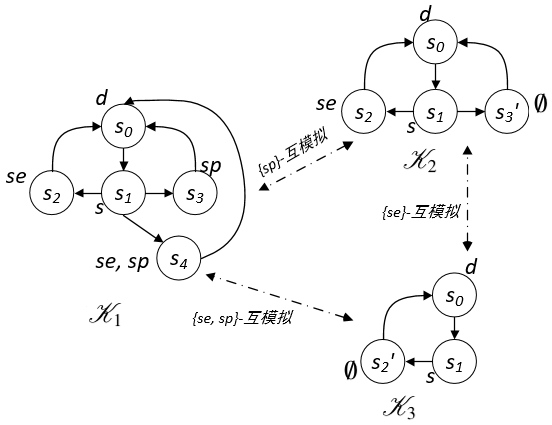
\includegraphics[width=8cm]{chapter03/NVBnewCar1.png}\\
		\caption{$\MPK$-结构之间的$V$-互模拟关系示意图}
		\label{Fig:chapter04:v1uv2}
	\end{figure*}
\end{example}



%$V$-互模拟给出了两个结构之间相互模仿的行为关系,下述命题给出了这种关系的一些关键性质。
下述命题给出了$V$-互模拟关系的一些关键性质。
\begin{proposition}\label{prop:bisimilar:V}
	给定集合$V_i\subseteq \Ha$、状态$s_i'$、路径$\pi_i'$和$\Ind$-结构${\cal K}_j=(\Hm_j,s_j)$,其中$i=1,2$,$j=1,2,3$。
	%令$i$是属于集合$\{1,2\}$的变量,$V_1$和$V_2$是$\Ha$的子集,$s_1'$和$s_2'$是两个状态,$\pi_1'$和$\pi_2'$是两条路径,${\cal K}_j=(\Hm_j,s_j)$$(j=1,2,3)$是$\Ind$-结构。
	如果${\cal K}_1 \lrto_{V_1} {\cal K}_2$且${\cal K}_2 \lrto_{V_2} {\cal K}_3$,则:
	\begin{itemize}
		\item[(i)] ${\cal K}_1\lrto_{V_1\cup V_2}{\cal K}_3$;
		\item[(ii)] 若 $V_1 \subseteq V_2$,则 ${\cal K}_1 \lrto_{V_2} {\cal K}_2$;
		\item[(iii)] $s_1'\lrto_{V_i}s_2'~(i=1,2)$ 蕴涵$s_1'\lrto_{V_1\cup V_2}s_2'$;
		\item[(iv)] $\pi_1'\lrto_{V_i}\pi_2'~(i=1,2)$ 蕴涵 $\pi_1'\lrto_{V_1\cup V_2}\pi_2'$;
		\item[(v)] 对$\Hm_1$上的每条路径 $\pi_{s_1}$,存在$\Hm_2$上的一条路径 $\pi_{s_2}$ 使得 $\pi_{s_1} \lrto_{V_1} \pi_{s_2}$,反之也成立。
	\end{itemize}
\end{proposition}
\begin{proof}
	%We prove the cases of $\MPK$-structures, and the cases of $\Ind$-structures are trivial.
	(i) 令 ${\cal M}_j=(S_j,R_j,L_j,[\_]_j,s_0^j)~(j=1,2,3)$,$\Hb$为$s_1$和$s_2$之间的$V_1$-互模拟关系,即 $s_1$ $\lrto_{V_1}$ $s_2$ 通过 $\Hb$形成$V_1$-互模拟关系,$s_2 \lrto_{V_2} s_3$通过$\Hb''$形成$V_2$-互模拟关系。 令 $\Hb' = \{(w_1,$ $w_3)\mid (w_1, w_2)\in \Hb$ 和 $(w_2, w_3)\in \Hb''\hbox{,其中}w_i\in S_i~(i=1,2,3)\}$。为了证明 ${\cal K}_1\lrto_{V_1\cup V_2}{\cal K}_3$,下证$\Hb'$ 是一个包含 $(s_1, s_3)$ 的 $V_1 \cup V_2$-互模拟关系。由于$(s_1,s_2)\in \Hb$ 和 $(s_2, s_3)\in \Hb''$,所以$(s_1, s_3) \in \Hb'$。
	% 		from the (a), (b) and (c) of the previous step (iii) of $X$-bisimulation (where $X$ is a set of atoms).
	对所有 $(w_1, w_3) \in \Hb'$,存在$w_2\in S_2$使得$(w_1, w_2)\in \Hb$和$(w_2, w_3)\in \Hb''$,且:
	\begin{itemize}
		\item[(a)] 存在一个 $w_2 \in S_2$使得 $(w_1,w_2)\in \Hb$ 且 $(w_2, w_3)\in \Hb''$。由 $w_1 \lrto_{V_1} w_2$可知;$L_1(w_1)$ $-V_1 = L_2(w_2) - V_1$;由$w_2 \lrto_{V_2} w_3$可知,$L_2(w_2) - V_2 = L_3(w_3) - V_2$。
		%			for all $q \notin V_1$, $q \in L_1(w_1)$ iff $q \in L_2(w_2)$ by $w_1 \lrto_{V_1} w_2$ and for all $q' \notin V_2$, $q'\in L_2(w_2)$ iff $q'\in L_3(w_3)$ by $w_2 \lrto_{V_2} w_3$. 
		所以,有 $L_1(w_1) - (V_1 \cup V_2) = L_3(w_3) - (V_1 \cup V_2)$。
		% for all $r\notin V_1 \cup V_2$, $r \in L_1(w_1)$ iff $r \in L_3(w_3)$.
		\item[(b)] $\forall u_1\in S_1$,若 $(w_1, u_1) \in R_1$,则 $\exists u_2\in S_2$ 使得$(w_2, u_2) \in R_2$ 和 $(u_1,u_2)\in \Hb$; 因而 $\exists u_3 \in S_3$ 使得$(w_3, u_3) \in R_3$ 且 $(u_2, u_3) \in \Hb''$,所以由 $\Hb'$的定义可知 $(u_1, u_3) \in \Hb'$。
		\item[(c)] $\forall u_3\in S_3$,若 $(w_3, u_3) \in R_3$,则 $\exists u_2\in S_2$ 使得 $(w_2, u_2) \in R_2$ 和 $(u_2, u_3) \in \Hb_2$;因此 $\exists u_1 \in S_1$ 使得  $(w_1, u_1) \in R_1$ 且 $(u_1, u_2) \in \Hb$,所以由 $\Hb'$的定义可知$(u_1, u_3) \in \Hb'$。
	\end{itemize}
	
	(ii) 假定 $\Hb_{V_1}$是$\Hm_1$ 和 $\Hm_2$之间的一个 $V_1$-互模拟关系,且 $(s_1, s_2)\in \Hb_{V_1}$。下证 $\Hb_{V_1}$ 也是$\Hm_1$ 和 $\Hm_2$之间的一个 $V_2$-互模拟关系。
	对任意 $(w_1, w_2) \in \Hb_{V_1}$,有:
	\begin{itemize}
		\item 因为$L_1(w_1) - V_1 = L_2(w_2) -V_1$ 和 $V_1 \subseteq V_2$,所以 $L_1(w_1) - V_2 = L_2(w_2) -V_2$;
		\item $\forall r_1 \in S_1$,若 $(w_1,r_1) \in R_1$,因为$\Hb_{V_1}$是$\Hm_1$ 和 $\Hm_2$之间的一个 $V_1$-互模拟关系, 则 $\exists r_2\in S_2$ 使得 $(w_2,r_2)\in R_2$ 且 $(r_1,r_2) \in \Hb_{V_1}$;
		\item $\forall r_2 \in S_2$,若 $(w_2,r_2) \in R_2$,因为$\Hb_{V_1}$是$\Hm_1$ 和 $\Hm_2$之间的一个 $V_1$-互模拟关系,则 $\exists r_1\in S_1$使得 $(w_1,r_1)\in R_1$ 且 $(r_1,r_2) \in \Hb_{V_1}$。
	\end{itemize}
	
	由于$V_i \subseteq (V_1 \cup V_2)$( $i = 1, 2$),则(iii)是 (ii)的一种特殊情况,因而(iv)从(iii)可以容易得到。
	
	(v) 因为$s_1 \lrto_{V_1} s_2$ (即:${\cal K}_1\lrto_{V_1}{\cal K}_2$),可以从$V$-互模拟的定义易证(v)。	
\end{proof}


在命题\ref{prop:bisimilar:V}中,性质(iii)-(v)的含义比较直观。性质(i)表示如果一个结构分别与另外的两个结构${\cal K}_1$和${\cal K}_3$具有$V_1$和$V_2$-互模拟关系,则${\cal K}_1$和${\cal K}_3$ 是 $V_1\cup V_2$-互模拟的(如图~\ref{Fig:chapter04:v1uv2}所示)。这一性质对遗忘性质的证明至关重要。性质(ii)表示若两个结构关于某一集合是互模拟的,则这两个结构关于该集合的超集是互模拟的。

从互模拟的定义来看,如果两个结构是$V$-互模拟的,那么对于与$V$中原子命题无关的公式$\varphi$来说,这两个结构同时满足或不满足$\varphi$。这一性质可以形式化地描述如下:

\begin{theorem}\label{thm:V-bisimulation:EQ}
	令$V\subseteq \Ha$是原子命题集,${\cal K}_i$ $(i=1,2)$是两个具有$V$-互模拟关系的$\Ind$-结构,即:${\cal K}_1 \lrto_V {\cal K}_2$。若$\Phi$是一个$\CTL$公式且$\IR(\Phi, V)$,则有${\cal K}_1\models \Phi$当且仅当${\cal K}_2\models \Phi$。
\end{theorem}
\begin{proof}
	下面通过归纳$\CTL$公式的结构证明这一结论。
	%这一结论可以从$\CTL$公式的结构归纳地来证明。此外,不失一般性地可以
	假设$\Var(\Phi) \cap V=\emptyset$,${\cal K}_1=(\Hm,s)$ 和 ${\cal K}_1=(\Hm',s')$。
	
	\textbf{基始.} $\Phi = p$ ($p\in \Ha -V$)。
	
	$(\Hm,s)\models \Phi$当且仅当$p\in L(s)$ \hfill (可满足关系的定义)\\
	$\LRto$ $p\in L'(s')$ \hfill ($s \lrto_V s'$)\\
	$\LRto$ $(\Hm',s') \models \Phi$。
	
	\textbf{归纳步.} (a) $\Phi = \neg \psi$。
	
	$(\Hm,s)\models \Phi$当且仅当$(\Hm,s) \not \models \psi$\\
	$\LRto$ $(\Hm',s')\not \models \psi$  \hfill (归纳假设)\\
	$\LRto$ $(\Hm',s') \models \Phi$。
	
	(b) $\Phi = \psi_1 \vee \psi_2$。
	
	$(\Hm,s)\models \Phi$\\
	$\LRto$ $(\Hm,s) \models \psi_1$或$(\Hm,s) \models \psi_2$\\
	$\LRto$ $(\Hm',s')  \models \psi_1$或$(\Hm',s') \models \psi_2$ \hfill (归纳假设)\\
	$\LRto$ $(\Hm',s') \models \Phi$。
	
	(c) $\Phi=\EXIST\NEXT\psi$。
	
	$(\Hm,s)\models \Phi$\\
	$\Rto$ 存在一条路径$\pi=(s,s_1,\dots)$使得$(\Hm,s_1)\models \psi$\\
	$\Rto$ 存在一条路径$\pi'=(s',s_1',\dots)$使得$\pi \lrto_V \pi'$且$(\Hm,s_1)\models \psi$\hfill ($s \lrto_V s'$,命题~\ref{prop:bisimilar:V})\\
	$\Rto$ $s_1 \lrto_V s_1'$且$(\Hm,s_1)\models \psi$ \hfill ($\pi \lrto_V \pi'$)\\
	$\Rto$ $(\Hm',s_1') \models \psi$   \hfill   (归纳假设)\\
	$\Rto$ $(\Hm',s')\models \Phi$。
	
	另一个方向可类似证明。
	
	(d) $\Phi = \EXIST \GLOBAL \psi$。
	
	$(\Hm,s)\models \Phi$\\
	$\Rto$ 存在一条路径$\pi=(s=s_0,s_1,\dots)$,使得对任意$i\ge 0$,都有$(\Hm,s_i)\models \psi$\\
	$\Rto$ 存在一条路径$\pi'=(s'=s_0',s_1',\dots)$,使得$\pi \lrto_V \pi'$,且对任意$i\ge 0$,都有$(\Hm,s_i)\models \psi$   \hfill ($s \lrto_V s'$,命题~\ref{prop:bisimilar:V})\\
	$\Rto$ 对于任意$i\ge 0$,都有$s_i \lrto_V s_i'$和$(\Hm,s_i)\models \psi$ \hfill ($\pi \lrto_V \pi'$)\\
	$\Rto$ 对于任意$i\ge 0$,都有$(\Hm,s_i') \models \psi$ \hfill (归纳假设)\\
	$\Rto$ $(\Hm',s')\models \Phi$。
	
	另一个方向可类似证明。
	
	(e) $\Phi = \EXIST (\psi_1 \UNTILL \psi_2)$。
	
	$(\Hm,s) \models \Phi$\\
	$\Rto$ 存在一条路径$\pi=(s=s_0,s_1,\dots)$和$i \ge 0$,使得$(\Hm,s_i) \models \psi_2$,且对所有的$0\leq j <i$都有$(\Hm,s_j)\models \psi_1$\\
	$\Rto$ 存在一条路径$\pi'=(s'=s_0',s_1',\dots)$,使得$\pi \lrto_V \pi'$和$(\Hm',s_i') \models \psi_2$,且对所有的$0\leq j <i$都有$(\Hm',s_j')\models \psi_1'$ \hfill ($s \lrto_V s'$,归纳假设,命题~\ref{prop:bisimilar:V})\\
	%$\Rto$ $(\Hm',s_i') \models \psi_2$,且对于所有的$0\leq j <i$,都有$(\Hm',s_j')\models \psi_1$  \hfill  \\
	$\Rto$ $(\Hm',s')\models \Phi$。
	
	另一个方向可类似证明。
\end{proof}

上述定理中,公式 $\Phi$不包含索引,否则, $\Ind$-结构中的索引函数可能会影响公式的可满足性。
例:令 $\phi=\EXIST_{\tuple{1}}\NEXT p$、
${\cal K}=(\Hm,s)$ 和 $\Hm=(S,R,L,[\_],s_0)$,其中 $S=\{s_0,s_1\}$, $L(s_0)=\emptyset$、 $L(s_1)=\{p\}$、
$R=\{(s_0,s_1),(s_0,s_0),(s_1,s_1), (s_1,s_0)\}$ 和 $[1]=\{(s_0,s_1), (s_1,s_1)\}$。显然,${\cal K}\models\phi$。
令 ${\cal K}'=(\Hm',s)$ 和 $\Hm'=(S,R,L,[\_]',s_0)$,其中 $[1]'=\{(s_0,s_0),(s_1,s_1)\}$。
显然,${\cal K}\lrto_{\{q\}}{\cal K}'$, $\IR(\phi,\{q\})$。但是,${\cal K}'\not\models\phi$。

\begin{example}
	令$\varphi_1 = d \wedge \EXIST\FUTURE se \wedge \ALL\GLOBAL(se \rto \ALL\NEXT d)$和$\varphi_2=d \wedge \ALL\NEXT se$是两个$\CTL$公式,且$\IR(\varphi_1,\{sp\})$ 和 $\IR(\varphi_2,\{sp\})$。因此,可以验证图\ref{Fig:chapter04:v1uv2}中的${\cal K}_1$和${\cal K}_2$都满足$\varphi_1$,但是都不满足$\varphi_2$。
\end{example}

\begin{definition}[互模拟等价,bisimilar equivalence]\label{def:bisimular:equivalene}
	给定原子命题集$V\subseteq {\cal A}$,公式$\varphi$和$\psi$。若对任意${\cal K}\models \varphi$,都存在一个${\cal K}'\models\psi$,使得${\cal K}\lrto_V{\cal K}'$;且对任意${\cal K}'\models\psi$,都存在一个${\cal K}\models \varphi$,使得${\cal K}\lrto_V{\cal K}'$,则称公式$\varphi$和 $\psi$是 {\em $V$-互模拟等价的(bisimilar equivalence)},记为 $\varphi\equiv_V\psi$。
\end{definition}

由定义\ref{def:VInd:bisimulation}和 \ref{def:bisimular:equivalene},和命题\ref{prop:bisimilar:V}可容易得出下列引理。
\begin{lemma}~\label{lem:eqR}
	对任意$V\subseteq\cal A$,  $\lrto_V$和 $\equiv_V$为等价关系。
\end{lemma}
\begin{proof}
	由命题\ref{prop:bisimilar:V}(i)可知 $\lrto_V$是传递的。显然也是自反和对称的。因此是等价关系。
	
	关系 $\equiv_V$显然是自反和对称的。
	假设$\varphi\equiv_V\psi$和 $\psi\equiv_V\xi$。则对任意 ${\cal K}\models\varphi$,由$\varphi\equiv_V\psi$可知,存在一个 ${\cal K}'\models\psi$使得${\cal K}'\lrto_V{\cal K}$;且由$\psi\equiv_V\xi$可知,存在一个 ${\cal K}''\models\xi$使得
	${\cal K}'\lrto_V{\cal K}''$。又因为$\lrto_V$是一个等价关系,因此,${\cal K}\lrto_V{\cal K}''$。类似地,对任意${\cal K}''\models\xi$,存在 ${\cal K}\models \varphi$ 使得${\cal K}''\lrto_V{\cal K}$。这表明$\equiv_V$是传递的。因此,$\equiv_V$是等价关系。
\end{proof} 


此外,由互模拟等价的定义和上述结论可得以下推论。%上面的定义和命题\ref{prop:bisimilar:V}蕴涵下面的推论。
% 	The below corollary follows from the above definition and Proposition~\ref{prop:bisimilar:V}.
\begin{corollary}~\label{cor:eqbi}
	令 $V$、$V_1$、$V_2$ 为$\cal A$的子集,$\varphi$和 $\psi$为公式。
	\begin{itemize}
		\item[(i)] 若 $\varphi\equiv\psi$,则 $\varphi\equiv_V\psi$。
		\item[(ii)] 若$\varphi$ 和 $\psi$不包括索引,且 $\varphi\equiv_\emptyset\psi$, 则 $\varphi\equiv\psi$。
		\item[(iii)] 若 $\varphi\equiv_{V_i}\psi~(i=1,2)$,则 $\varphi\equiv_{V_1\cup V_2}\psi$。
		\item[(iv)] 若 $\varphi\equiv_{V_1}\psi$ 和 $V_1\subseteq V_2$,则 $\varphi\equiv_{V_2}\psi$。
	\end{itemize}
\end{corollary}
\begin{proof}
	(i) 对任意$\varphi$(或 $\psi$)的模型 ${\cal K}$和$V \subseteq \Ha$,存在${\cal K} \lrto_V {\cal K}$。因此, $\varphi\equiv_V\psi$。
	
	(ii) 对任意$\varphi$的模型${\cal K}$,存在$\psi$的一个模型${\cal K}'$使得 ${\cal K} \lrto_{\emptyset} {\cal K}'$。显然 $\IR(\psi, \emptyset)$,由定理~\ref{thm:V-bisimulation:EQ}可知${\cal K} \models \psi$。类似地,对任意${\cal K}' \models \psi$,存在${\cal K} \models \varphi$使得 ${\cal K} \lrto_{\emptyset} {\cal K}'$,因此${\cal K}'\models \varphi$。
	
	(iii) 对任意${\cal K} \models \varphi$,存在${\cal K}' \models \psi$,使得 ${\cal K} \lrto_{V_i} {\cal K}'$ ($i=1,2$)。因此,由命题\ref{prop:bisimilar:V}(i)可知 ${\cal K} \lrto_{V_1\cup V_2} {\cal K}'$。类似地,对任意${\cal K}' \models \psi$,存在 ${\cal K} \models \varphi$,使得${\cal K} \lrto_{V_1\cup V_2} {\cal K}'$。因此,$\varphi\equiv_{V_1\cup V_2}\psi$。
	
	同理可证(iv)。
\end{proof}

请注意,在上述结论(ii)中  “$\varphi$和$\psi$不包含索引”是必要的。否则,令 $\varphi=\EXIST_{\tuple{1}}\NEXT p$ 和  
$\psi$ $=\EXIST_{\tuple{2}}\NEXT p$,可以证明,$\varphi\equiv_\emptyset \psi$,但是 $\varphi\not\equiv\psi$。
\begin{proposition}\label{prop:transform:V:EQ}
	令 $\varphi$为一个$\CTL$公式。则$\varphi\equiv_UT_\varphi$,其中 $T_\varphi=\CTLsnf(\varphi)$和
	$U=\Var(T_\varphi)-\Var(\varphi)$。
\end{proposition}
\begin{proof}
	令$T_0, T_1, \dots, T_n=T_{\varphi}$为转换过程产生的公式集合序列。$T_0=\{\ALL \GLOBAL(\start \rto p), \ALL \GLOBAL(p \rto \simp(\nnf(\varphi)))\}$,其中$p$是不出现在$\varphi$中的原子命题,且对任意$i$($0\leq i < n$),有$T_{i+1} = (T_i-\{\psi\}) \cup R_i$($Trans(\psi)$返回的结果为$R_i$)。此外,在这一过程中,所有公式都是否定范式形式。
	
	为了证明命题中的结论,只需证明,对任意$i$($0\leq i < n$),$T_i \equiv_{U} T_{i+1}$成立。由于$T_{i+1}$是由$T_i$通过表\ref{tab:trans}中的规则作用于$T_i$中的某一个公式得到,因此证明过程分为两个部分:(1)从$\varphi$到$T_0$部分;(2)从$T_0$到$T_{\varphi}$的部分。假设$\Hm_1=(S_1,R_1,L_1,[\_]_1,s_1)$和$\Hm_2=(S_2,R_2,L_2, [\_]_2, s_2)$。
	
	(1)下证$\varphi \equiv_{\{p\}} T_0$。
	
	$(\Rto)$ $\forall (\Hm_1, s_1) \in \Mod(\varphi)$,可以构造一个$\Ind$-Kripke结构$\Hm_2=(S_2,R_2,L_2,[\_],s_2)$,使得除了$L_2(s_2)=L_1(s_1) \cup \{p\}$(默认不出现在$\varphi$中的原子命题都不出现在状态的标签中),$\Hm_2$中的其它元素都与$\Hm_1$中的元素相同。显然,$(\Hm_2,s_2)\models T_0$且$(\Hm_1,s_1) \lrto_{\{p\}} (\Hm_2, s_2)$。
	
	$(\Lto)$ $\forall (\Hm_1,s_1) \in \Mod(T_0)$,由$\start$的语义可知$(\Hm_1,s_1) \models \varphi$。
	
	(2)下证对任意$i$($0\leq i < n$),有$T_i \equiv_{U} T_{i+1}$成立,其中$T_{i+1} = (T_i-\{\psi\}) \cup R_i$。这里,用$\psi \rto_t R_i$表示$R_i$是使用规则$t$在公式$\psi$上得到的结果,且$T_i=X\cup \{\psi\}$(显然,$T_{i+1}=X\cup R_i$,$X=T_i-\{\psi\}$)。下面证明规则$t\in \{$\textbf{Trans(1), Trans(4), Trans(6)}$\}$的情形,其它情形可以类似地证明。
	
	(a)$t=\textbf{Trans(1)}$。
	
	$(\Rto)$ $(\Hm_1,s_1)\in \Mod(T_i)$,即$(\Hm_1, s_1) \models X \wedge \ALL\GLOBAL(q \rto \EXIST \NEXT \varphi)$\\
	$\Rto$ $(\Hm_1,s_1) \models X$,且对任意路径$\pi=(s_{1,1},s_{1,2},\dots)$上的状态$s_{1,j}$ $(j\geq 1)$,有$(\Hm,s_{1,j}) \not \models \neg q$,或存在一个状态$s_{1,j+1}$使得$(s_{1,j},s_{1,j+1})
	\in R_1$且$(\Hm,s_{1,j+1}) \models \varphi$。
	
	由此构造一个初始$\Ind$-Kripke结构$\Hm_2$,使得$\Hm_2$与$\Hm_1$相同,除了:对使用规则 \textbf{Tra- ns(1)} 在公式$\ALL\GLOBAL(q \rto \EXIST \NEXT \varphi)$上而引入的新索引$ind$,有$[ind]_2=\bigcup_{s\in S} R_s \cup R_y$。其中:
	\begin{itemize}
		\item $R_{s_{1,j}}=\{(s_{1,j}, s_{1,j+1}), (s_{1,j+1}, s_{1,j+2}),\dots\}$ $(j\geq 1)$,其满足“若$(\Hm_1,s_{1,j}) \models q$,则$(\Hm_1,$ $s_{1,j+1})$ $\models \varphi$”且“对于任意$i\geq j$,若$(s_{1,i}, s') \in R_s\ (s \not= s_{1,j})$,则$s'=s_{1,i+1}$”;
		\item $R_y=\{(s_x,s_y)\mid s_x\in S$,若对任意$(s_1',s_2') \in \bigcup_{s\in S} R_s$, 有$s_1'\not= s_x$,则找一个状态$s_y\in S_2$,使得$(s_x,s_y)\in R_2\}$。
	\end{itemize}
	
	显然,$(\Hm_1,s_1) \lrto_{\emptyset} (\Hm_2,s_2)$\\
	$\Rto$ 对任意从$s_2$开始的路径$\pi=( s_2= s_{2,1} , s_{2,2}, \dots)$,如果$s_{2,j} \in \pi$,则$(\Hm_2,s_{2,j}) \models \neg q$或$(\Hm_2,$ $s_{2,j})\models \EXIST_{\tuple{ind}} \NEXT \varphi$\\
	$\Rto$ $(\Hm_2,s_2)\models \ALL\GLOBAL(q \rto \EXIST_{\tuple{ind}} \NEXT \varphi)$\\
	$\Rto$ $(\Hm_2,s_1) \models X \wedge \ALL\GLOBAL(q \rto \EXIST_{\tuple{ind}} \NEXT \varphi)$
	
	$(\Lto)$ $\forall (\Hm_1,s_1) \in \Mod(T_{i+1})$,即$(\Hm_1,s_1) \models X \wedge \ALL \GLOBAL(q \rto \EXIST_{\tuple{ind}} \NEXT \varphi )$\\
	$\Rto$ $(\Hm_1,s_1) \models X$且$(\Hm_1,s_1) \models \ALL \GLOBAL(q \rto \EXIST_{\tuple{ind}} \NEXT \varphi)$\\
	$\Rto$ 对任意以$s_1$为起点的路径上的任意状态$s_{1,j}$,$(\Hm_1,s_{1,j}) \models \neg q$或$(\Hm_1,s_{1,j}) \models \EXIST\NEXT\varphi$\\
	$\Rto$ $(\Hm_1,s_1) \models \ALL\GLOBAL(q \rto \EXIST \NEXT \varphi)$\\
	$\Rto$ $(\Hm_1,s_1) \models X \wedge \ALL\GLOBAL(q \rto \EXIST \NEXT \varphi)$。
	
	(b)$t=\textbf{Trans(4)}$。
	
	$(\Rto)$	$(\Hm_1,s_1) \in \Mod(T_i)$,即$(\Hm_1,s_1) \models X \wedge \ALL\GLOBAL (q \rto \varphi_1 \vee \varphi_2)$ \\
	$\Rto$ $(\Hm_1,s_1) \models X$,且$\forall s_1'\in S_1$,$(\Hm_1, s_1') \models q \rto \varphi_1 \vee \varphi_2$\\
	$\Rto$ $(\Hm_1,s_1')\models \neg q$或$(\Hm_1,s_1')\models \varphi_1 \vee \varphi_2$。
	
	如下构造初始$\Ind$-Kripke结构$\Hm_2=(S_2,R_2,L_2,[\_]_2,s_2)$:
	\begin{itemize}
		\item $S_2=S_1$,$R_2=R_1$,$[\_]_2$与$[\_]_1$相同,且$s_2=s_1$;
		\item $L_2$与$L_1$相同,除了:对任意$s_1'\in S_2$,若$(\Hm_1, s_1') \models \neg q$,则$L_2(s_1') = L_1(s_1')$,否则“若$(\Hm_1,s_1') \models \varphi_1$,则 $L_2(s_1')=L_1(s_1')$,否则$L_2(s_1')=L_1(s_1') \cup \{p\}$”。
	\end{itemize}
	显然,$(\Hm_2,s_1') \models (q\rto \varphi_1 \vee p) \wedge (p \rto \varphi_2)$且$(\Hm_1, s_1) \lrto_{\{p\}} (\Hm_2, s_2)$,所以,$(\Hm_2,s_2) \models T_{i+1}$。
	
	$(\Lto)$  $\forall (\Hm_1, s_1) \in \Mod(T_{i+1})$,即$(\Hm_1,s_1) \models X \wedge \ALL\GLOBAL (q\rto \varphi_1 \vee p) \wedge \ALL\GLOBAL(p \rto \varphi_2)$。 显然,$(\Hm_1, s_1) \models T_i$。
	
	(c)$t$=\textbf{Trans(6)}。
	
	这里证明$\EXIST_{\tuple{ind}} \NEXT$的情形,$\ALL \NEXT$的情形可以类似地证明。
	
	$(\Rto)$ $(\Hm_1,s_1) \in \Mod(T_i)$,即$(\Hm_1,s_1) \models X \wedge \ALL\GLOBAL(q \rto \EXIST_{\tuple{ind}}\NEXT \varphi)$\\
	$\Rto$ $(\Hm_1,s_1) \models X$,且对任意$s_1'\in S$,$(\Hm_1,s_1') \models q \rto \EXIST_{\tuple{ind}} \NEXT \varphi$\\
	$\Rto$ $(\Hm_1,s_1') \models \neg q$,或者存在一个状态$s'$,使得$(s_1', s') \in [ind]$且$(\Hm_1,s') \models \varphi$。
	
	如下构造初始$\Ind$-Kripke结构$\Hm_2=(S_2,R_2,L_2,[\_]_2,s_2)$:
	\begin{itemize}
		\item $S_2=S_1$,$R_2=R_1$,$[\_]_2$与$[\_]_1$一样且$s_2=s_1$;
		\item $L_2$与$L_1$相同,除了:对任意$s_1'\in S_2$,若$(\Hm_1, s_1') \models \neg q$,则$L_2(s_1') = L_1(s_1')$,否则“若$(\Hm_1,s_1') \models q$,则$L_2(s')$ $=L_1(s')\cup \{p\}$ $((s_1',s')\in R_2)$”。
	\end{itemize}
	显然,$(\Hm_2,s_2) \models \ALL\GLOBAL(q\rto \EXIST_{\tuple{ind}} \NEXT p) \wedge \ALL\GLOBAL(p \rto \varphi)$、$(\Hm_2,s_2) \models T_{i+1}$且$(\Hm_1, s_1) \lrto_{\{p\}} (\Hm_2, s_2)$ ($s_2=s_1$)。
	
	$(\Lto)$ $(\Hm_1, s_1) \in \Mod(T_{i+1})$,即$(\Hm_1,s_1) \models X \wedge \ALL\GLOBAL(q\rto \EXIST_{\tuple{ind}} \NEXT p) \wedge \ALL\GLOBAL(p \rto \varphi)$。显然,$(\Hm_1, s_1) \models T_i$。
\end{proof}
 
\begin{example}
	\label{examp:Tran}
	令 $\varphi=\ALL((p\wedge q) \UNTILL (f\vee m)) \wedge r$。 $T_{\varphi}$是下面子句构成的集合:
	\begin{align*}
		&  1: \start\rto z, &&  2: \top \rto \neg z \vee r, &&  3:\top \rto \neg x\vee f \vee m, &&
		4: \top \rto \neg z \vee x \vee y, \\
		&  5: \top \rto \neg y \vee p, &&  6: \top \rto \neg y \vee q, &&  7:  z \rto \ALL \FUTURE x, &&  8: y \rto \ALL \NEXT(x\vee y)
	\end{align*}
	其中 $x,y,z$ 为新引入的原子命题。
	%	$
	%	\begin{array}{llll}
	%		1. \start\rto z & 2. \top \rto \neg z \vee r \qquad & 3.\top \rto \neg x\vee f \vee m  & 4. \top \rto \neg z \vee x \vee y \\
	%		5.\top \rto \neg y \vee p &  6.\top \rto \neg y \vee q &
	%		7. z \rto \ALL \FUTURE x & 8. y \rto \ALL \NEXT(x\vee y),\\
	%	\end{array}
	%	$\\
	%	with the set $V'=\{x, y,z\}$ of new atoms introduced in this process, in which $w$ is a new atom related to $z \rto \ALL \FUTURE x$
	%~\footnote{Note that we always generate a new atom $w$ for each $Q$-sometime clause with $Q\in \{\EXIST, \ALL\}$ when this clause is produced during the transformation process.}. %~\cite{zhang2014resolution}.
	% Besides, the set of new atoms introduced in this process is $V'=\{x, y,z, w\}$ in which $w$ is a new atom related to $z \rto \ALL \FUTURE x$~\footnote{Note that we always generate a new atom for each $T$-sometime clause with $T\in \{\EXIST, \ALL\}$ when this clause is produced during the transform process.}. %~\cite{zhang2014resolution}.
\end{example}

\subsection{遗忘算子及其性质}
这部分给出$\CTL$遗忘的定义及其相关性质。

\begin{definition}[遗忘,forgetting]\label{def:V:forgetting}
	令$V$是$\Ha$的子集,$\Phi$是公式。如果公式$\psi$满足下面条件:
	%,记为$\CTLforget(\Phi, V)$:
	\begin{itemize}
		\item $\psi$与$V$中的原子命题无关(即:$\IR(\psi, V)$);
		\item $\Mod(\psi)=\{{\cal K}\mid {\cal K} \mbox{是一个初始$\Ind$-结构}, \exists {\cal K}'\in\Mod(\phi)\ \text{使得}\ {\cal K}'\lrto_V{\cal K}\}$。
	\end{itemize}
	%$V$中原子命题无关的公式(即:$\Var(\varphi) \cap V= \emptyset$) 
	那么,称$\psi$为从$\Phi$中遗忘$V$后得到的结果。
\end{definition}


从定义\ref{def:V:forgetting}可以看出,如果两个公式$\psi$和$\psi'$都是$\Phi$遗忘$V$中元素后得到的结果,则$\Mod(\psi)\equiv \Mod(\psi')$。从这个角度来看,$\Phi$遗忘$V$中元素后得到的所有结果是语义等价的。
将遗忘结果记为$\CTLforget(\phi,V)$,不做其它说明的情况下,这表示$\phi$遗忘$V$是$\CTL$可表示的。
此外,当$V$中只包含一个元素时,可以省略集合符号,即:$$\CTLforget(\Phi, \{p\}) \equiv \CTLforget(\Phi, p).$$ 

%值得指出的是,遗忘理论的定义与均匀插值的语义定义等价,也即是遗忘理论与均匀插值是一对对偶概念,这与其他逻辑(包括模态逻辑S4、S5和经典命题逻辑)中的说法一致~\cite{gfdf}。


遗忘的定义表明,如果公式$\psi$的任意一个模型${\cal K}$都能找到$\varphi$的一个模型${\cal K}'$使得${\cal K} \lrto_V {\cal K}'$,那么称$\psi$为$\varphi$遗忘$V$中原子命题后得到的结果。为刻画S5逻辑下遗忘的直观含义,Zhang等人提出了遗忘的特性——这些特性被称为\emph{遗忘理论公设}(forgetting postulates)~\cite{Yan:AIJ:2009}。
类似地,给定$\CTL$公式$\varphi$、$\varphi'=\CTLforget(\varphi, V)$、原子命题集$V\subseteq \Ha$和$\varphi'=\CTLforget(\varphi, V)$,$\CTL$下遗忘理论公设如下:
\begin{itemize}
	\item[(\W)] 削弱:$\varphi \models \varphi'$;
	\item[(\PP)] 正支持:对任意与$V$无关的公式$\eta$,若$\varphi \models \eta$则$\varphi' \models \eta$;
	\item[(\NgP)] 负支持:对任意与$V$无关的公式$\eta$,若$\varphi \not \models \eta$则$\varphi' \not \models \eta$;
	\item[(\textbf{IR})] 无关性: $\IR(\varphi', V)$。
\end{itemize}
其中(\W)和(\textbf{IR})表明,“遗忘”削弱了公式$\varphi$,且得到的结果与$V$无关;(\PP)和(\NgP)表明,对任意与$V$无关的公式$\eta$,$\varphi \models \eta$当且仅当$\varphi' \models \eta$。总而言之,遗忘结果能蕴涵所有与$V$无关且能被$\varphi$蕴涵的结果,不能蕴涵所有与$V$无关且不能被$\varphi$蕴涵的结果。
此外,这些公设不都是独立的(如:$\NP$由$\W$和$\PP$可以得出),但这里把它们都列出来以表达更加直观的含义。
从数据库和安全的层面讲,遗忘相当于从已有的关系表中构建一个视图,达到隐私保护的作用。
下面的定理表明上述公设对$\CTL$的遗忘是充分且必要的。
%下面的定理表明$\CTL$中的遗忘与上述公设也具有当且仅当的关系。

\begin{theorem}[表达性定理,Representation Theorem]\label{thm:close}
	%Let $\varphi$, $\varphi'$ and $\phi$ be \CTL\
	给定$\CTL$公式$\varphi$和$\varphi'$,$V \subseteq \Ha$为原子命题集。
	%Then t
	下面的陈述是等价的:
	\begin{itemize}
		\item[(i)] $\varphi' \equiv \CTLforget(\varphi, V)$,
		\item[(ii)] $\varphi'\equiv \{\phi \mid\varphi \models \phi \text{和} \IR(\phi, V)\}$,
		\item[(iii)] 若$\varphi$、$\varphi'$和$V$为(i)和(ii)中提到的符号,则公设(\W)、(\PP)、(\NgP)和(\textbf{IR})成立。
	\end{itemize}
\end{theorem}
\begin{proof}
	$(i) \LRto (ii)$. 通过证明如下等式证明该结论。%为了证明这个结论,只需证明如下等式成立:
	\[
	\Mod(\CTLforget(\varphi, V)) = \Mod(\{\phi \mid \varphi \models \phi, \IR(\phi, V)\}).\]
	$(\Rto)$ ${\cal K}'\models\CTLforget(\varphi, V)$\\
	$\Rto$  $\exists {\cal K}$使得${\cal K} \models \varphi$且${\cal K} \lrto_V {\cal K}'$ \hfill (定义~\ref{def:V:forgetting}) \\
	$\Rto$ $\forall \phi$,若$\varphi \models \phi$且$\IR(\phi, V)$,则${\cal K}' \models \phi$  \hfill (定理~\ref{thm:V-bisimulation:EQ})\\
	$\Rto$ ${\cal K}' \models \{\phi \mid \varphi \models \phi, \IR(\phi, V)\}$
	
	$(\Lto)$ 因为$\IR(\CTLforget(\varphi, V),V)$且$\varphi \models \CTLforget(\varphi, V)$,由定义~\ref{def:V:forgetting}可知$\{\phi \mid \varphi \models \phi, \IR(\phi, V)\} \models \CTLforget(\varphi, V)$。
	
	$(ii) \Rto (iii)$. 令$A = \{\phi \mid \varphi \models \phi, \IR(\phi, V)\}$。 
	首先,由于对任意$\phi'\in A$,都有$\varphi \models \phi'$,所以,$\varphi \models \varphi'$。
	其次,对任意公式$\phi$,若$\IR(\phi, V)$且$\varphi \models \phi$,则$\phi \in A$,因此,$\varphi' \models \phi$。
	第三, 对任意公式$\phi$,若$\IR(\phi, V)$且$\varphi \not \models \phi$,则$\phi \not \in A$。因此,$\varphi' \not \models \phi$。
	最后,因为对任意$\phi' \in A$,都有$\IR(\varphi',V)$ ,所以,$\IR(\phi',V)$。
	
	$(iii) \Rto (ii)$. 一方面,由(\PP) 和 (\NgP)可知,对任意公式$\phi'$且$\IR(\phi',V)$,$\varphi \models \phi'$当且仅当$\varphi' \models \phi'$。所以,对任意$\phi'\in \{\phi \mid \varphi \models \phi, \IR(\phi, V)\}$,都有$\varphi' \models \phi'$,所以,$\varphi' \models \{\phi \mid \varphi \models \phi, \IR(\phi, V)\}$。 
	另一方面,由 (\W) 和 (\textbf{IR})可知,$\{\phi \mid \varphi \models \phi, \IR(\phi, V)\} \models \varphi'$。因此,$\varphi'\equiv \{\phi \mid\varphi \models \phi, \IR(\phi, V)\}$。
\end{proof}

定理~\ref{thm:close}并不表明遗忘的结果一定存在。
%尽管上面的表达性定理描述了遗忘及其基本准则之间“当且仅当”的关系,值得注意的是上面的定义~\ref{def:V:forgetting}并不表示遗忘的结果一定存在。
事实上,存在一个$\CTL$公式和原子命题集,使得从该公式里遗忘该集合得到的结果不可用$\CTL$公式表达。
例:令$p$和 $x$为两个不同的原子命题,$\varphi(p,x)$\footnote{$\varphi(p,x)$ 表示具有原子命题集$\Var(\varphi)=\{p,x\}$的公式。}为下面公式合取~\cite{Maksimova:JANCL:1991}:
\begin{align*}
	&\ALL\GLOBAL(\neg x \wedge \neg \ALL \GLOBAL p \rto \neg \ALL \NEXT \neg x),
	\qquad \ALL\GLOBAL(\neg \ALL\NEXT \neg x \rto \ALL \NEXT x),\\
	& \ALL\GLOBAL(\ALL\NEXT x \rto \neg x \wedge \neg \ALL \GLOBAL p),
	\qquad \ALL\GLOBAL(x \rto \neg \ALL\GLOBAL p),
	\qquad \ALL\GLOBAL(\ALL \FUTURE \ALL \GLOBAL p).
\end{align*}
\citeauthor{Maksimova:JANCL:1991}证明了$\varphi(p,x)\land \varphi(p,y)\models x\lrto y$,且不存在$\CTL$公式 $\psi$使得 $\Var(\psi)=\{p\}$且$\varphi(p,x)$ $\models x\lrto \psi$,即$\CTL$不具有Beth性质。
这一结论蕴涵如下命题:
\begin{proposition}\label{pro:uniforget}
	$\CTLforget(x\land \varphi(p,x), \{x\})$ 在 $\CTL$中是不可表示的。
\end{proposition}
\begin{proof}
	令 $\psi(p)=\CTLforget(x\land \varphi(p,x), \{x\})$为一个$\CTL$公式。
	有 \\
	$\varphi(p,x)\land \varphi(p,y)\vdash x\lrto y$\\
	$\Rto$ $\varphi(p,x)\land x \vdash \varphi(p,y)\rto y$\\
	$\Rto$ $\varphi(p,x)\land x\vdash \psi(p)$ 和 $\psi(p)\vdash \varphi(p,y)\rto p(y)$\hfill (定理~\ref{thm:close})\\
	$\Rto$ $\varphi(p,x)\vdash x\rto\psi(p)$且$\varphi(p,y)\vdash \psi(p)\rto p(y)$,这表明$\varphi(p,x)\vdash \psi(p)\rto p(x)$\\
	$\Rto$ $\varphi(p,x)\vdash x\lrto \psi(p)$,这是一个矛盾。
\end{proof}




从命题公式$\varphi$中遗忘原子命题$p$为:$\Forget(\varphi,\{p\})\equiv\varphi[p/\bot] \vee \varphi[p/\top]$。
本文遗忘的定义对公式为命题逻辑公式时,与Lin等人于1994提出的命题逻辑遗忘一致,即:本文的$\CTL$遗忘扩展了命题逻辑遗忘。%下面命题展示了上述结论:

\begin{theorem}\label{thm:PL:CTL}
	给定一个命题公式$\varphi$和原子命题集$V\subseteq \Ha$,则下面逻辑等式成立。
	\[\CTLforget(\varphi, V) \equiv \Forget(\varphi,V).
	\]
\end{theorem}
\begin{proof}
%	为了证明上述结论成立,只需要证明$\Mod(\CTLforget(\varphi, V))= \Mod(\Forget(\varphi,V))$。	
	一方面,对于$\CTLforget(\varphi, V)$的任意一个模型$(\Hm, s)$,由遗忘的定义可知存在一个$\varphi$的模型$(\Hm',s')$使得$(\Hm, s)\lrto_V (\Hm',s')$。因而有$L(s)-V = L'(s')-V$(其中$L\in \Hm$,$L'\in \Hm'$),这表明$(\Hm,s)\models \Forget(\varphi,V)$。
	
	另一方面,对于$\Forget(\varphi,V)$的任意一个模型$(\Hm, s)$($\Hm=(S,R,L,[\_],s)$),存在$\varphi$的一个模型$(\Hm',s')$($\Hm'=(S',R',L',[\_]',s')$),使得$L(s)-V = L'(s')-V$。如下构建一个初始$\Ind$-结构$(\Hm_1,s_1)$,使得$\Hm_1=(S_1,R_1,L_1,[\_],s_1)$,其中:
	\begin{itemize}
		\item $S_1=(S-\{s\})\cup \{s_1\}$;
		\item $R_1$由将$R$出现的$s$替换为$s_1$得到;
		\item 对于$S_1$中任意一个状态$s^*$:
		\[L_1(s^*)=
		\left\{
		\begin{array}{ll}
			L'(s'), \quad \qquad \qquad \hbox{如果$s^*=s_1$;} \\
			L(s^*), \ \ \ \ \qquad \qquad \hbox{否则。}
		\end{array}
		\right.
		\]
	\end{itemize}
	
	显然,$(\Hm_1,s_1)$是$\varphi$的一个模型且$s_1 \lrto_V s$。因此,$(\Hm,s)$是$\CTLforget(\varphi,V)$的一个模型。
\end{proof}

遗忘的另一个重要性质与$V$-无关性密切相关。对于给定的公式$\psi=\varphi \wedge (q\lrto \alpha)$,如果$\IR(\varphi \wedge \alpha, \{q\})$,那么$\psi$遗忘$q$后得到的结果为$\varphi$。这一性质与后文将要介绍的$SNC$($WSC$)的计算密切相关。但是,由于其也是遗忘的性质,因而本文将其放在此处。
\begin{lemma}\label{lem:KF:eq}
	给定两个公式$\varphi$和$\alpha$,原子命题$q \not \in (\Var(\varphi) \cup \Var(\alpha))$,则:$$\CTLforget(\varphi \wedge (q \lrto \alpha), q)\equiv \varphi.$$
\end{lemma}
\begin{proof}
	$(\Rto)$ 令$\varphi'=\varphi \wedge (q \lrto \alpha)$。
	对于$\CTLforget(\varphi',q)$的任意模型$(\Hm,s)$,由遗忘的定义可知存在一个初始$\Ind$-结构$(\Hm',s')$,使得$(\Hm,s)\lrto_{\{q\}}(\Hm',s')$且$(\Hm',s')\models \varphi'$。
	显然,$(\Hm',s')\models \varphi$。
	此外,由于$\IR(\varphi, \{q\})$且$(\Hm,s)\lrto_{\{q\}}(\Hm',s')$,由定理~\ref{thm:V-bisimulation:EQ}可知$(\Hm,s)\models \varphi$。
	
		$(\Lto)$  令$\Hm=(S,R,L,[\_],s)$且$(\Hm,s)\in \Mod(\varphi)$。下面构造初始$\Ind$-结构$(\Hm',s)$,使得$\Hm'=(S,R,L',[\_],s)$,其中:
	\begin{align*}
		& L':S \rto 2^{\Ha}\ \mbox{且}\ \forall s^*\in S, \hbox{ 若}\ (\Hm, s^*) \not \models \alpha, \hbox{ 则 } L'(s^*) = L(s^*)-\{q\}\,  \hbox{ 否则 }\ L'(s^*) = L(s^*)\cup\{q\}, \\
		& \hbox{ 若}\ (\Hm, s) \models \alpha, \hbox{ 则 } L'(s) = L(s) \cup\{q\}, \ \hbox{ 否则}\ L'(s) = L(s)-\{q\}.
	\end{align*}
	
	显然,$(\Hm',s) \models \varphi$、$(\Hm',s)\models q \lrto \alpha$且$(\Hm',s) \lrto_{\{q\}} (\Hm,s)$。
	因此,$(\Hm',s) \models \varphi \wedge (q \lrto \alpha)$。所以,由$(\Hm',s) \lrto_{\{q\}} (\Hm,s)$可知,$(\Hm,s)\models \CTLforget(\varphi \wedge (q \lrto \alpha), q)$。
\end{proof}

%除了上述性质,遗忘还有其它一些一般性质。下面将详细介绍这些性质。

根据遗忘的定义可以看出,从一个公式里遗忘某个原子命题集中的元素是将该集合看作一个整体来遗忘的。下面的结论说明,遗忘原子命题集可分解为遗忘单个原子命题。
%遗忘可以将原子命题中的元素拿出来一个一个的遗忘,而不是作为一个整体。
\begin{proposition}[分解性,Decomposition]\label{disTF}
	对于给定的公式$\varphi$,原子命题集$V$,和原子命题$p$($p\not \in V$),下面的结论成立:
	\[
	\CTLforget(\varphi,\{p\}\cup V) \equiv \CTLforget(\CTLforget(\varphi,p),V).
	\]
\end{proposition}
\begin{proof}
%	要证明上述结论成立,只需证明等式左右两边的公式有相同的模型。	
	一方面,令$\Hm_1=(S_1,R_1,L_1,[\_],s_1)$是一个初始$\Ind$-Kripke结构,且$(\Hm_1,s_1)$是$\CTLforget(\varphi,$ $\{p\}\cup V)$的一个模型。由遗忘的定义可知,存在$\varphi$的一个模型$(
	\Hm,s)$($\Hm=(S,R,L,[\_],s)$)使得$(\Hm_1,s_1)\lrto_{\{p\}\cup V} (\Hm,s)$。
	如下构建一个初始$\Ind$-结构$(\Hm_2,s_2)$,使得$\Hm_2=(S_2,R_2,L_2,$ $[\_],s_2)$且:
	\begin{itemize}
		\item[(1)] 对于$s_2$情形:令$s_2$是满足下面条件的状态,
		\begin{itemize}
			\item $p \in L_2(s_2)$当且仅当$p\in L_1(s_1)$,
			\item 对任意$q \in V$,$q \in L_2(s_2)$当且仅当$q\in L(s)$,
			\item 对其它原子命题$q'$,$q' \in L_2(s_2)$,当且仅当$q'\in L_1(s_1)$,当且仅当$q'\in L(s)$。
		\end{itemize}
		
		\item[(2)] 其它情形:
		\begin{itemize}
			\item 对所有状态对$(w,w_1)$,若$w\in S$,$w_1\in S_1$且$w\lrto_{\{p\}\cup V} w_1$,如下构造$w_2\in S_2$:%对于所有的满足$w\in S$,$w_1\in S_1$且$w\lrto_{\{p\}\cup V} w_1$的状态对$(w,w_1)$,如下构造$w_2\in S_2$:
			\begin{itemize}
				\item $p \in L_2(w_2)$当且仅当$p\in L_1(w_1)$,
				\item 对任意$q \in V$,$q \in L_2(w_2)$当且仅当$q\in L(w)$,
				\item 对其它原子命题$q'$,$q' \in L_2(w_2)$,当且仅当$q'\in L_1(w_1)$,当且仅当$q'\in L(w)$。
			\end{itemize}
			\item 对于$(w_1',w_1)\in R_1$,若$w_2$由$w_1$构造而成,且$w_2'$由$w_1'$构造而成,则令$(w_2',w_2)\in R_2$。
		\end{itemize}
		\item[(3)] 删除$S_2$和$R_2$中重复的元素。
	\end{itemize}
	由此可知,$(\Hm, s) \lrto_{\{p\}} (\Hm_2, s_2)$且 $(\Hm_2, s_2) \lrto_V (\Hm_1, s_1)$。 所以,$(\Hm_2, s_2) \models \CTLforget(\varphi, p)$。 因此, $(\Hm_1,$ $s_1) \models \CTLforget(\CTLforget(\varphi, p), V)$。
	
	另一方面,若$(\Hm_1, s_1)$是$\CTLforget(\CTLforget(\varphi, p), V)$的一个模型,则存在一个初始-$\Ind$结构 $(\Hm_2, s_2)$,使得 $(\Hm_2, s_2) \models \CTLforget(\varphi, p)$且 $(\Hm_2, s_2) \lrto_V (\Hm_1, s_1)$;且存在 $(\Hm, s)$,使得$(\Hm,$ $s) \models \varphi$且 $(\Hm, s) \lrto_{\{p\}} (\Hm_2, s_2)$。因此,由命题~\ref{prop:bisimilar:V}(i)可知 $(\Hm, s) \lrto_{\{p\} \cup V} (\Hm_1, s_1)$,所以, $(\Hm_1,$ $s_1)$ $\models \CTLforget(\varphi, \{p\} \cup V)$。
\end{proof}

由上面的命题不难看出,从公式中遗忘原子命题集中的元素,可以将该集合拆成两个集合遗忘。
\begin{corollary}
	对于给定的公式$\varphi$,原子命题集$V_1$和$V_2$,有如下结论:
	\[
	\CTLforget(\varphi,V_1\cup V_2) \equiv \CTLforget(\CTLforget(\varphi,V_1),V_2).
	\]
\end{corollary}

类似于被遗忘的原子命题集能被拆成两个集合的遗忘,下面介绍在某些情况下,从带时序算子的公式中遗忘一些原子命题,可以将这些时序算子提到遗忘操作的前面。
\begin{proposition}
	令$V\subseteq \Ha$为原子命题集,$\phi$为$\CTL$公式,则下面等式成立:
	\begin{itemize}
		\item[(i)] $\CTLforget(\ALL\NEXT\phi,V) \equiv \ALL \NEXT\CTLforget(\phi,V)$;
		\item[(ii)] $\CTLforget(\EXIST\NEXT\phi,V) \equiv \EXIST \NEXT\CTLforget(\phi,V)$;
		\item[(iii)] $\CTLforget(\ALL\FUTURE\phi,V) \equiv \ALL\FUTURE\CTLforget(\phi,V)$;
		\item[(iv)] $\CTLforget(\EXIST\FUTURE\phi,V) \equiv \EXIST\FUTURE\CTLforget(\phi,V)$;
		\item[(v)] $\CTLforget(\ALL \GLOBAL\phi,V)\equiv \ALL \GLOBAL\CTLforget(\phi,V)$;
		\item[(vi)] $\CTLforget(\EXIST\GLOBAL\phi,V)\equiv\EXIST\GLOBAL \CTLforget(\phi,V)$。
	\end{itemize}
\end{proposition}
\begin{proof}
	(i) $(\Rto)$ $(\Hm,s)\models\CTLforget(\ALL\NEXT\phi,V)$\\
	$\Rto$ 存在$(\Hm,s)\lrto_V(\Hm',s')$且 $(\Hm',s')\models \ALL\NEXT\phi$\\
	$\Rto$  $(\Hm,s)\lrto_V(\Hm',s')$,且 对任意$(s',s'')\in R'$,有$(\Hm',s'')\models \phi$ \hfill ($R'\in\Hm'$)\\
	$\Rto$ 对任意$(s,s_1)\in R$,存在$(s',s'_1)\in R'$,使得$(\Hm,s_1)\lrto_V(\Hm',s'_1)$,且对任意$(s',s'')\in R'$,有
	$(\Hm',s'')\models \phi$\\
	$\Rto$ 对任意$(s,s_1)\in R$,有$(\Hm,s_1)\lrto_V(\Hm',s'_1)$且$(\Hm',s'_1)\models\phi$\\
	$\Rto$ 对任意$(s,s_1)\in R$, $(\Hm,s_1)\models\CTLforget(\phi,V)$\\
	$\Rto$ $(\Hm,s)\models\ALL\NEXT\CTLforget(\phi,V)$。
	
	$(\Lto)$ $(\Hm,s)\models\ALL\NEXT\CTLforget(\phi,V)$\\
	$\Rto$ 对任意$(s,s')\in R$, 有$(\Hm,s')\models\CTLforget(\phi,V)$ \hfill ($R\in \Hm)$\\
	$\Rto$ 对任意$(s,s')\in R$, 有$(\Hm,s')\lrto_V(\Hm',s'')$且$(\Hm',s'')\models\phi$\\
	$\Rto$ 对任意$i\ge 0$,有$(\Hm,s'_i)\lrto_V(\Hm'_i,s''_i)$且 $(\Hm'_i,s''_i)\models\phi$,
	其中 $\{s'_0,s'_1,\ldots\}=\{s'\mid (s,s')\in R\}$且 $\Hm'_i=(S'_i,R'_i,L'_i,[\_]'_i,s''_i)$ \hfill (当$i\neq j$时,假定$S'_i\cap S'_j=\emptyset$)\\
	$\Rto$ $(\Hm^*,s)\lrto_V(\Hm,s)$ 且 $(\Hm^*,s)\models\ALL\NEXT\phi$,其中
	$\Hm^*=(S^*,R^*,L^*,[\_], s)$且
	\begin{itemize}
		\item $S^*=\{s\}\cup\bigcup_{i\ge 0}S'_i$,
		\item $R^*=\{(s,s''_i)\mid i\ge 0\}\cup \bigcup_{i\ge 0} R'_i$,
		\item $L^*=\bigcup_{i\ge 0}L'_i$ 和 $L^*(s)=L(s)$,其中 $L\in\Hm$。
	\end{itemize}
	$\Rto$ $(\Hm,s)\models \CTLforget(\ALL\NEXT\phi,V)$。
	
	(ii) $(\Rto)$ $(\Hm,s)\models\CTLforget(\EXIST\NEXT\phi,V)$\\
	$\Rto$ 存在$(\Hm,s)\lrto_V(\Hm',s')$ 且 $(\Hm',s')\models \EXIST\NEXT\phi$\\
	$\Rto$ 存在$(\Hm,s)\lrto_V(\Hm',s')$,且对一些 $(s',s'')\in R'$,有$(\Hm',s'')\models \phi$ \hfill  ($R'\in\Hm'$)\\
	$\Rto$ 存在$(s,s_1)\in R$和$(s',s'_1)\in R'$,使得$(\Hm,s_1)\lrto_V(\Hm',s'_1)$,且存在$(s',s'')\in R'$,使得
	$(\Hm',$ $s'')\models \phi$ \hfill ($R\in \Hm$)\\
	$\Rto$ 存在$(s,s_1)\in R$和$(\Hm,s_1)\lrto_V(\Hm',s'_1)$,使得$(\Hm',s'_1)\models\phi$\\
	$\Rto$ 存在$(s,s_1)\in R$,使得$(\Hm,s_1)\models\CTLforget(\phi,V)$\\
	$\Rto$ $(\Hm,s)\models\EXIST\NEXT\CTLforget(\phi,V)$。
	
	$(\Lto)$ $(\Hm,s)\models\EXIST \NEXT\CTLforget(\phi,V)$\\
	$\Rto$ 对一些 $(s,s')\in R$, $(\Hm,s')\models\CTLforget(\phi,V)$  ($R\in \Hm)$\\
	$\Rto$ 对一些 $(s,s')\in R$,有$(\Hm,s')\lrto_V(\Hm',s'')$ 和 $(\Hm',s'')\models\phi$,其中 $\Hm'=(S',R',L',[\_]',s'')$ \\
	%		$\Rto$ For every $i\ge 0$, there is $(\Hm,s'_i)\lrto_V(\Hm'_i,s''_i)$ and $(\Hm'_i,s''_i)\models\phi$
	%		where $\{s'_0,s'_1,\ldots\}=\{s'\mid (s,s')\in R\}$ and $\Hm'_i=(S'_i,R'_i,L'_i,[\_]'_i,s''_i)$ (we assume $S'_i\cap S'_j=\emptyset$ when $i\neq j$)\\
	$\Rto$ $(\Hm^*,s)\lrto_V(\Hm,s)$ 和 $(\Hm^*,s)\models\EXIST\NEXT\phi$,其中
	$\Hm^*=(S^*,R^*,L^*,[\_], s)$,
	\begin{itemize}
		\item $S^*=S\cup S'$,
		\item $R^*=\{(s,s'')\}\cup R \cup R'$,
		\item $L^*= L \cup L'$ 且$L^*(s)=L(s)$,其中 $L\in\Hm$。
	\end{itemize}
	$\Rto$ $(\Hm,s)\models \CTLforget(\EXIST\NEXT\phi,V)$。
	
	
	
	
	(iii)和 (iv)可以分别类似 (i)和 (ii)来证明。
	
	(v) $(\Rto)$ $(\Hm,s) \models \CTLforget(\ALL \GLOBAL \phi, V)$\\
	$\Rto$ 存在$(\Hm',s') \models \ALL \GLOBAL \phi$且 $(\Hm,s) \lrto_V (\Hm',s')$\\
	$\Rto$ 对$\Hm$上的每一条路径$\pi=(s=s_1, s_2, \dots)$,存在$\Hm'$上的一条路径$\pi'=(s'=s_1, s_2', \dots)$,使得 $\pi \lrto_V \pi'$,反之也成立,且对任意$i\geq 1$,有$(\Hm', s_i') \models \varphi$\\ 
	%$\Rto$ For every $t' \in S'$, there is $(\Hm',t') \models \phi$ \quad ($S'\in \Hm'$) \\
	% $\Rto$ For every $t' \in S'$, there is $(\Hm',t') \models \CTLforget(\phi, V)$\\
	% $\Rto$ For every $t \in S$, there is $(\Hm,t) \models \CTLforget(\phi, V)$ \quad ($S\in \Hm$) \hfill ($\IR(\CTLforget(\phi, V), V)$)\\
	$\Rto$ 对$\pi$上的任意$s_i'$($i\geq 1$),有$(\Hm',s_i') \models \CTLforget(\phi, V)$\\
	$\Rto$ 对$\pi'$上的任意$s_i$($i\geq 1$),有$(\Hm,s_i) \models \CTLforget(\phi, V)$ \hfill ($\IR(\CTLforget(\phi, V), V)$)\\
	$\Rto$ 对任意$t \in S$,有$(\Hm,t) \models \CTLforget(\phi, V)$ \hfill ($S\in \Hm$)\\
	$\Rto$ $(\Hm,s) \models \ALL \GLOBAL \CTLforget(\phi, V)$。
	
	$(\Lto)$ $(\Hm, s) \models \ALL \GLOBAL \CTLforget(\phi, V)$\\
	$\Rto$ 对$\Hm$上的每一条路径 $\pi=(s=s_0, s_1, \dots)$,和任意$i \geq 0$,有$(\Hm,s_i) \models \CTLforget(\phi, V)$  \\ 
	$\Rto$ $\forall t \in S$, $(\Hm,t) \models \CTLforget(\phi, V)$ \hfill ($S \in \Hm$)\\
	$\Rto$ $\forall t \in S$,有$(\Hm,t) \lrto_V (\Hm',t')$且$(\Hm',t') \models \phi$\\
	$\Rto$ $\forall s_i \in S$ ($i \geq 0$),有$(\Hm,s_i) \lrto_V (\Hm_i',s_i')$且 $(\Hm_i',s_i') \models \phi$,其中$\Hm_i' = (S_i',R_i', L_i', [\_]_i',s_i')$\\
	$\Rto$ $(\Hm^*,s^*) \lrto_V (\Hm,s)$和$(\Hm^*,s^*) \models \ALL \GLOBAL \phi$,其中$\Hm^*= (S^*, R^*,L^*, [\_], s^*)$,
	\begin{itemize}
		\item $S^*= \bigcup S_i'$, %\{s_i \mid i \geq 0\}$,
		\item $s* = s_0'$,
		\item $R^* = \{(s_x', s_y') \mid (s_x, s_y) \in R,\ x, y \geq 0\} \cup \bigcup_{i \geq 0} R_i'$,其中 $R\in \Hm$,
		\item 对任意$t_i\in S_i'$,$L^*(t_i) = L_i'(t_i)$。
	\end{itemize}
	$\Rto$ $(\Hm,s) \models \CTLforget(\ALL \GLOBAL \phi, V)$。
	
	(vi) 可类似 (v)来证明。
\end{proof}


\begin{corollary}
	给定命题集合$V\subseteq \Ha$,命题公式$\varphi$和$\CTL$公式$\ALL\GLOBAL \psi$,则
	$$\CTLforget(\varphi \wedge \ALL\GLOBAL \psi)\equiv \CTLforget(\varphi \wedge \psi, V) \wedge \ALL\GLOBAL\CTLforget(\psi, V).$$
\end{corollary}
\begin{proof}
	 $(\Hm,s_0) \models \CTLforget(\varphi \wedge \ALL\GLOBAL \psi)$\\
	$\LRto$ 存在$(\Hm',s_0')  \lrto_V (\Hm,s_0)$,使得$(\Hm',s_0') \models \varphi \wedge \ALL\GLOBAL \psi$\\
	$\LRto$ 存在$(\Hm',s_0')  \lrto_V (\Hm,s_0)$,使得$(\Hm',s_0') \models \varphi \wedge \psi$且$(\Hm',s_0') \models \ALL\GLOBAL \psi$\\
	$\LRto$% 存在$(\Hm',s_0')  \lrto_V (\Hm,s_0)$,
	$(\Hm,s_0) \models \CTLforget(\varphi \wedge \psi,V)$且$(\Hm,s_0) \models \CTLforget(\ALL\GLOBAL \psi,V)$\\
%	$\LRto$ 存在$(\Hm',s_0')  \lrto_V (\Hm,s_0)$,使得$(\Hm',s_0') \models \CTLforget(\varphi \wedge \psi,V)$且$(\Hm',s_0') \models \ALL\GLOBAL\CTLforget( \psi,V)$\\
	$\LRto$ $(\Hm,s_0) \models \CTLforget(\varphi \wedge \psi,V)\wedge \ALL\GLOBAL\CTLforget( \psi,V)$。
\end{proof}
\section{$\mu$-演算遗忘理论}
\label{chapter03:sec:muforget}
$\mu$-演算是一种表达能力较强的逻辑语言,它能表达$\CTL$不能表达的一些性质,例如:Kripke结构中有一条路径,在这条路径上,基数位置的状态满足公式$\neg q \wedge \neg p$,但是偶数位置的状态满足$q \wedge p$。这一性质不能用$\CTL$公式来表达,但是可以用$\mu$-演算公式表达如下:
$$\varphi = \nu X.(p \wedge q) \wedge \EXIST \NEXT(\neg p \wedge \neg q) \wedge \EXIST \NEXT \EXIST \NEXT X.$$

这种情形在日常生活中是很常见的,如:偏序关系$(\mathbb{N}, \leq)$(自然数集上的小于等于关系)构成的Kripke结构,其基数节点为基数、偶数节点为偶数。
事实上,$\CTL$不能表达具有有规律的性质~\cite{DBLP:journals/iandc/Wolper83},其主要原因是
\begin{quote}
	\emph{对于给定的原子命题$p$,任意包含$n$个“$\NEXT$”时序算子的命题时序公式( proposinal temporal formula,PTL),对序列“$p^i(\neg p) p^w$”有相同的真值,其中$i > n$。%Given a proposition $p$, any proposinal temporal formula (PTL) $f(p)$ containing 
		%n ``next" ($\NEXT$) operators has the same truth value on all sequences of the form 
		%$p^i(\neg p) p^w$, $i > n$.
	}
\end{quote}

因而得出如下结论:
\begin{quote}
	\emph{对任意$m\geq 2$,性质“$p$在所有状态$s_i$上为真($i = k*m$,整数$k\geq 0$)”不能用PTL中的公式来表示。
		%For any given $m\geq 2$, the property ``$p$ is true in every 
		%state $s_i$, where $i = km$ (integer $k\geq 0$)" is not expressible in PTL.
	}
\end{quote}





本小节给出$\mu$-演算遗忘的定义,并说明本文所定义的$\mu$-演算遗忘与文章~\cite{d2006modal}中定义的均匀插值具有对偶关系。此时,本文给出的遗忘性质也是均匀插值所具有的性质,这为$\mu$-演算均匀插值的探索提供了另一种思路。此外,借助于均匀插值的计算方法,本文给出计算遗忘的方法。形成了遗忘和均匀插值之间相辅相成的作用。

本小节的组织结构如下。首先,给出变元-命题-互模拟的定义及证明变元-命题-互模拟对$\mu$-公式是不变的;根据变元-命题-互模拟定义$\mu$-演算遗忘;然后,探讨遗忘的性质,并给出其与均匀插值的关系;最后给出与遗忘相关问题的复杂性。

\subsection{变元-命题-互模拟}
与$\CTL$遗忘相似,这里先给出$V$-互模拟的定义。令$\Hm_i = (S_i, R_i, L_i, r_i)$,$i$为自然数集$\mathbb{N}$中的元素。
\begin{definition}[$V$-互模拟]\label{def:VB}
	给定原子命题集$V \subseteq \Ha$和两个Kripke结构$\Hm_1$和 $\Hm_2$。若$\Hb\subseteq S_1 \times S_2$满足下面几个条件:
	\begin{itemize}
		\item $r_1 \Hb r_2$,
		\item 对任意$s\in S_1$和 $t\in S_2$,若$s \Hb t$,则对任意$p \in \Ha- V$,有$p \in L_1(s)$当且仅当 $p \in L_2(t)$,
		\item 若$(s, s')\in R_1$和 $s \Hb t$,则存在一个 $t'$,使得$s' \Hb t'$和 $(t, t')\in R_2$,且
		\item 若 $s \Hb t$和$(t, t')\in R_2$,则存在一个$s'$,使得$(s, s')\in R_1$和 $t' \Hb s'$。
	\end{itemize}
则称$\Hb$是$\Hm_1$和 $\Hm_2$的$V$-互模拟关系。
\end{definition}

一方面,与$\CTL$下的$V$-互模拟不同的是:这里要求$r_1 \Hb r_2$(即:$(r_1,r_2)\in \Hb$)。
如果$\Hm_1$和 $\Hm_2$之间存在一个$V$-互模拟关系,那么${\cal B}$则称这两个Kripke结构$\Hm_1$和 $\Hm_2$及由这两个Kripke结构构成的结构$(\Hm_1,r_1)$和$(\Hm_2,r_2)$是$V$-互模拟的,分别记为$\Hm_1 \lrto_V \Hm_2$和$(\Hm_1,$ $r_1) \lrto_V (\Hm_2,r_2)$。
显然,Kripke结构之间的$V$-互模拟与结构之间的$V$-互模拟是等价的:$\Hm_1 \lrto_V \Hm_2$当且仅当$(\Hm_1,r_1) \lrto_V (\Hm_2,r_2)$。 因此,在下文中只讨论Kripke结构之间$V$-互模拟的性质,而结构之间的互模拟的性质与之相同。不难看出初始结构之间的$V$-互模拟是结构之间的$V$-互模拟的一个特例。


另一方面,$V$-互模拟与${\cal L}$-互模拟
%\footnote{${\cal L}$-互模拟是一种将定义\ref{def:VB}中的$V$替换为${\cal L}$的二元关系。}
~\cite{d1996uniform}类似,不同的是$V$-互模拟只考虑原子命题,且当${\cal L}$为原子命题集时是${\cal L}$-互模拟补命题(这里默认除了原子命题之外的符号都是相同的,因此只考虑原子命题)。
此外,已有结果表明${\cal L}$-句子(符号只出现在${\cal L}$中的$\mu$-句子)关于${\cal L}$-互模拟是{\em 不变的},即若$\Hm$和 $\Hm'$是${\cal L}$-互模拟的,则对于${\cal L}$-句子$\varphi$有$\Hm \models \varphi$当且仅当$\Hm' \models \varphi$~\cite{d1996uniform,bradfield2018mu}。
因此,若$\IR(\varphi, V)$且$\Hm \lrto_V \Hm'$,则$\Hm \models \varphi$当且仅当$\Hm' \models \varphi$。
本文称这一性质为$V$-不变性。
%值得注意的是这里的结构之间的$V$-互模拟是$\CTL$
%In this case, $\Hm_1$ and $\Hm_2$ are bisimilar on $V$.
\begin{example}\label{exmp:c06:bisim}
	 令$\varphi= \nu X.( ch \wedge j \wedge  \EXIST \NEXT \EXIST \NEXT X)$,易证下面两个赋值$(\Hm,v)$和$(\Hm',v')$(图~\ref{chapter06:fig:bisim}中的两个Kripke结构)
	 是$\varphi$的模型,其中
	\begin{itemize}
		\item $\Hm=(S,r,R,L)$,其中$S=\{s_0,s_1,s_2\}$,$r=s_0$,$L(s_0)=\{ch, j\}$,$L(s_1)=\{ch\}$,$L(s_2)=\emptyset$,$R=\{(s_0,s_1), (s_1,s_0), (s_0,s_2), (s_2,s_0)\}$,$v(X)=\{s_0\}$,
		\item  $\Hm'=(S',r',R',L')$,其中$S'=\{t_0,t_1\}, r'=t_0$,$L'(t_0)=\{j\}$,$L'(t_1)=\emptyset$,$R'=\{(t_0,t_1),$ $(t_1,$ $t_0)\}$且
		$v'(X)=\{t_0\}$。
	\end{itemize} 
	
		\begin{figure}[h]%
		\centering
		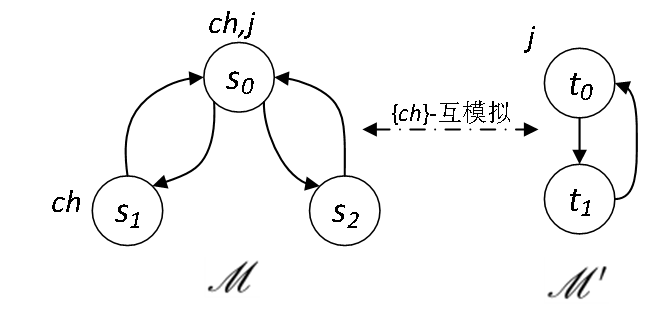
\includegraphics[width=5cm]{chapter06/chvB3.png}
		\caption{两个 $\{ch\}$-互模拟的Kripke结构示意图}\label{chapter06:fig:bisim}
		
		% $s_0$ is labeled by $\{ch, j\}$, $t_0$ is labeled by $\{j\}$, and $s_1$, $s_2$, and $t_1$ are labeled by $\emptyset$.}\label{fig:bisim}
	\end{figure}
	
	由于$\Hm$和 $\Hm'$之间存在一个$\{ch\}$-互模拟关系$\Hb=\{(s_0, t_0), (s_1, t_1), (s_2, t_1)\}$,所以,$\Hm \lrto_{\{ch\}}$ $\Hm'$。
\end{example}
%\begin{example}
%	\label{exmp:c06:bisim}
%	如图\ref{chapter06:fig:bisim}中的两个Kripke结构$\Hm=(S,R,L,r)$和 $\Hm'=(S',R',L',r')$,其中:
%	\begin{itemize}
%		\item $S=\{s_0,s_1,s_2\}$,$S'=\{t_0,t_1\}$,$r=s_0$,$r'=t_0$;
%		\item $R=\{(s_0,s_1),(s_1,s_0),(s_0,s_2),(s_2,s_0)\}$,$R'=\{t_0,t_1\}$;
%		\item $L(s_0)=\{ch,j\}$,$L(s_1)=\{ch\}$,$L(s_2)=\emptyset$,$L'(t_0)=\{j\}$,$L'(t_1)=\emptyset$。
%	\end{itemize}
%	由于$\Hm$和 $\Hm'$之间存在一个二元$\{ch\}$-互模拟$\Hb=\{(s_0, t_0), (s_1, t_1), (s_2, t_1)\}$,所以 $\Hm \lrto_{\{ch\}} \Hm'$。%,所以$\Hm\lrto \Hm'$。
%	
%	
%	
%	% 	\begin{center}\label{fig:bisim}
%	% 		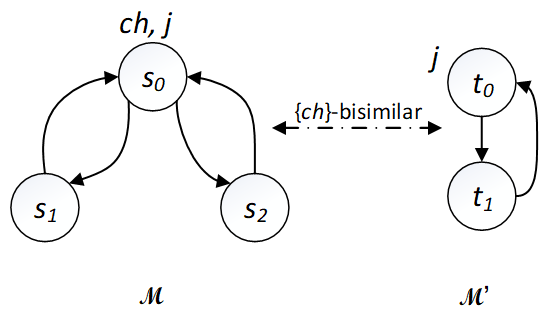
\includegraphics[width=5cm,height=3cm]{chBisimilar.png}\\
%	% 		%\vspace{2mm}
%	% 		\parbox[c]{7cm}{\textbf{Fig.1~}  Two $\{ch\}$-bisimilar Kripke structures}%\vspace*{.2mm}
%	% 	\end{center}
%	
%	\begin{figure}[h]%
%		\centering
%		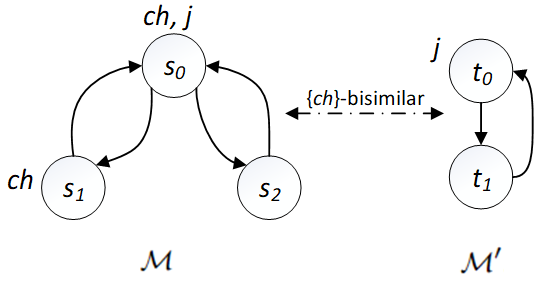
\includegraphics[width=4.5cm,height=2.5cm]{chapter06/chvB1.png}
%		\caption{两个 $\{ch\}$-互模拟的Kripke结构示意图}\label{chapter06:fig:bisim}
%		
%		% $s_0$ is labeled by $\{ch, j\}$, $t_0$ is labeled by $\{j\}$, and $s_1$, $s_2$, and $t_1$ are labeled by $\emptyset$.}\label{fig:bisim}
%	\end{figure}
%	
%\end{example}

$\mu$-句子互模拟是不变的,$\mu$-公式则不是~\cite{janin1996expressive}。这里定义一种对$\mu$-公式是不变的互模拟。

\begin{definition}[变元-命题-互模拟]
	给定$V \subseteq \Ha$、${\cal V}_1 \subseteq {\cal V}$、$\Hm_i = (S_i, r_i, R_i, L_i)$为Kripke结构、 $s_i\in S_i$且
	$v_i: {\cal V} \rto 2^{S_i}$,其中$i\in\{1,2\}$。若关系$\Hb\subseteq S_1 \times S_2$满足:
	\begin{itemize}
		\item $(s_1,s_2)\in\Hb$,
		\item $\Hb$是$\Hm_1$ 和$\Hm_2$之间的$V$-互模拟,且
		\item 对任意$(t_1,t_2)\in \Hb$和$X  \in {\cal V}-{\cal V}_1$,$t_2\in v_2(X)$当且仅当$t_1 \in v_1(X)$。
	\end{itemize}	
则称$\Hb$是$(\Hm_1,s_1, v_1)$ 和$(\Hm_2,s_2, v_2)$之间的一个{\em $\tuple{{\cal V}_1, V}$-互模拟}。
\end{definition}
%
%\begin{definition}[Var-$V$-互模拟]
%	\label{def:varVb}
%	给定原子命题集合$V$、赋值$(\Hm, v)$和$(\Hm',v')$。$(\Hm, v)$和$(\Hm',v')$之间的一个Var-$V$-互模拟关系$\Hb$是$\Hm$和$\Hm'$之间一个$V$-互模拟关系,且满足:
%	若 $(s,s') \in {\cal B}$,则对任意$X\in {\cal V}$, $s\in v(X)$ 当且仅当 $s'\in v'(X)$。
%\end{definition}

若$(\Hm,s, v)$和$(\Hm',s',v')$之间存在一个$\tuple{{\cal V}_1, V}$-互模拟关系$\Hb$,则称$(\Hm,s, v)$和$(\Hm',s',$ $v')$是$\tuple{{\cal V}_1, V}$-互模拟的,记为$(\Hm,s, v)\lrto_\tuple{{\cal V}_1, V} (\Hm',s',v')$。
若$(\Hm,s, v)$和$(\Hm',s',v')$之间存在一个$\tuple{\emptyset, V_1}$-互模拟关系,则称$(\Hm,s, v)$和$(\Hm',s',v')$是{\em Var-$V_1$-互模拟的},记为$(\Hm, s,v) $ $\lrto_{V_1} (\Hm',s',v')$;称$\tuple{\emptyset, V_1}$-互模拟为Var-$V_1$-互模拟。此外,若$s=r$ 且$s'=r'$,则$(\Hm, s,v) $ $\lrto_{\tuple{{\cal V}_1, V}} (\Hm',s',v')$简写为$(\Hm, v) \lrto_{\tuple{{\cal V}_1, V}} (\Hm',v')$。

显然,若$({\cal M},s,v)\lrto_V({\cal M}',s',v')$,则${\cal M}\lrto_V{\cal M}'$。
$\Hm\lrto_V\Hm'$,但$(\Hm,v)\not\lrto_V(\Hm',v')$ 有时是成立的。例:例~\ref{exmp:c06:bisim}中的两个Kripke结构$\Hm$ 和 $\Hm'$ 是$\emptyset$-互模拟的。然而,由于$r_1\in v(X)$和$(r_1,r_2')\in\Hb$,但是$r_2'\not\in v'(X)$,所以$(\Hm,v)\not\lrto_\emptyset (\Hm',v')$。
对$S_1\subseteq S$和二元关系$\Hb\subseteq S \times S'$,记$\Hb(S_1) =\{s' \mid (s, s')\in \Hb,\ s \in S_1\}$。

再者,对任意$X\in {\cal V}$,令$v(X)=S$且$v'(X)=S'$,Kripke结构${\cal M}$和${\cal M}'$之间的任意$V$-互模拟可以容易地扩展为$({\cal M},r,v)$和$({\cal M}',r',v')$之间的Var-$V$-互模拟,其中$S$和$S'$分别为$\Hm$和$\Hm'$中的状态集合。

\begin{example}[例~\ref{exmp:c06:bisim}的延续]
	令 $\Hm$和 $\Hm'$为图~\ref{chapter06:fig:bisim}中的Kripke结构,$v: {\cal V} \rto 2^S$和$v': {\cal V} \rto 2^{S'}$为将${\cal V}$中的变元分别赋值到$\Hm$和$\Hm'$的状态集上的赋值函数。可以检查下面的结论成立:
	\begin{itemize}
		\item 若对任意$X\in\cal V$,$v(X)= \{s_0, s_1, s_2\}$ 且$v'(X)=\{t_0, t_1\}$,则$({\cal M},v)\lrto_{\{ch\}} ({\cal M}',v')$;
		
		\item 若对任意$X\in{\cal V}-\{X_1\}$,$v(X_1)= \{s_0\}$、$v'(X_1)=\{t_1\}$、$v(X)= \{s_0, s_1, s_2\}$且$v'(X)=\{t_0, t_1\}$,则$({\cal M},v)\not\lrto_{\{ch\}} ({\cal M}',v')$;这是因为$(s_0,t_0)\in {\cal B}$且 $s_0\in v(X_1)$,但是$t_0\notin v'(X_1)$。
	\end{itemize}
\end{example}



可以证明$\lrto_V$有如下性质。

\begin{proposition} \label{pro:EqUnion}
	令${\cal V}_1, {\cal V}_2\subseteq {\cal V}$、$V, V_1 \subseteq \Ha$且$\Hm_i$为Kripke结构($i=1,2,3$),若$v_i: {\cal V}\rto 2^{S_i}$,则:
	\begin{enumerate} [(i)]
		\item $\lrto_{\tuple{{\cal V}_1,V}}$为赋值间的等价关系;
		\item 若$(\Hm_1, s_1,v_1) \lrto_{\tuple{{\cal V}_1,V}} (\Hm_2,s_2,v_2)$、${\cal V}_1 \subseteq {\cal V}_2$且$V \subseteq V_1$,\\
		则 $(\Hm_1, s_1, v_1) \lrto_{\tuple{{\cal V}_2,V_1}} (\Hm_2, s_2, v_2)$;
		\item 若$(\Hm_1, s_1, v_1) \lrto_{\tuple{{\cal V}_1,V}} (\Hm_2,s_2, v_2)$且$(\Hm_2,s_2, v_2) \lrto_{\tuple{{\cal V}_2,V_1}} (\Hm_3,s_3, v_3)$,\\
		则 $(\Hm_1,s_1,v_1) \lrto_{\tuple{{\cal V}_1 \cup {\cal V}_2, V \cup V_1}} (\Hm_3,s_3,v_3)$。
	\end{enumerate}
%	令$V, V_1 \subseteq \Ha$为原子命题集,$(\Hm_1,v_1)$、 $(\Hm_2,v_2)$和$(\Hm_3,v_3)$为赋值,则:
%	\begin{itemize} 
%		\item[(i)] $\lrto_V$是 赋值之间的等价关系;
%		\item[(ii)] 若$(\Hm_1, v_1) \lrto_V (\Hm_2,v_2)$ 和$V \subseteq V_1$,则$(\Hm_1, v_1) \lrto_{V_1} (\Hm_2,v_2)$;
%		\item[(iii)] 若 $(\Hm_1, v_1)  \lrto_V (\Hm_2,v_2)$且 $(\Hm_2,v_2) \lrto_{V_1} (\Hm_3,v_3)$,则 $(\Hm_1, v_1) \lrto_{V \cup V_1} (\Hm_3,v_3)$。
%	\end{itemize}
%	
\end{proposition}
\begin{proof}
%	Let $\Hm_i = (S_i, r_i, R_i, L_i)$ be Kripke structures, and $v_i: {\cal V} \rto 2^{S_i}$ be valuations of the variables in ${\cal V}$ to the states of $\Hm_i$ ($i=1,2,3$).
	
	(i) 这里从自反性、对称性和传递性来证明该关系是一个等价关系。
	
	(a) $\lrto_V$是自反的。显然,对任意的赋值$(\Hm,s,v)$都有$(\Hm,s,v)\lrto_{\tuple{{\cal V}_1,V}} (\Hm,s,v)$。
	
	(b) 对称性: % $\lrto_V$ is symmetric. 
	下证对任意$(\Hm_1,s_1, v_1)$和$(\Hm_2,s_2,v_2)$,若$(\Hm_1,s_1, v_1) \lrto_{\tuple{{\cal V}_1,V}} (\Hm_2,s_2,v_2)$,则$(\Hm_2,s_2, v_2) \lrto_{\tuple{{\cal V}_1,V}} (\Hm_1,s_1, v_1)$。
	假定$(\Hm_1, s_1,v_1)$ 和$(\Hm_2,s_2,v_2)$ 有${\tuple{{\cal V}_1,V}}$-互模拟关系$\Hb$,如下构造关系$\Hb_1$:$\Hb_1=\{(s,t) \mid (t, s)\in \Hb\hbox{,其中 } t\in S_1 \hbox{和} s\in S_2\}$。下证$\Hb_1$是$\Hm_2$$\Hm_1$之间的$V$-互模拟关系。
	\begin{itemize}
		\item 因为 $(r_1,r_2) \in \Hb$,所以,$(r_2,r_1) \in \Hb_1$;
		\item 对任意$s\in S_2$ 和$t\in S_1$,若$(s,t) \in \Hb_1$,则$(t,s) \in \Hb$。因此,对任意$p \in \Ha - V$,$p \in L_1(t)$当且仅当$p \in L_2(s)$;
		\item 因为$\Hb$是$\Hm_1$和 $\Hm_2$之间的$V$-互模拟关系,所以$V$-互模拟的第三和第四个点很容易能够证明。
	\end{itemize}
	此外,若$(t,s) \in \Hb$,则对任意$X\in {\cal V} -{\cal V}_1$,$s \in v_1(X)$ 当且仅当$t \in v_2(X)$。因此,若$(s,t) \in \Hb_1$, 则对任意$X\in {\cal V} -{\cal V}_1$,$t \in v_2(X)$ 当且仅当$s\in v_1(X)$。所以, $(\Hm_2,s_2, v_2) \lrto_{\tuple{{\cal V}_1,V}} (\Hm_1,s_1, v_1)$。

	(c) 传递性:%$\lrto_V$ is transitive. 
	下证若$(\Hm_1,s_1,v_1) \lrto_{\tuple{{\cal V}_1,V}} (\Hm_2,s_2,v_2)$和$(\Hm_2,s_2,v_2) \lrto_{\tuple{{\cal V}_1,V}} (\Hm_3,s_3,v_3)$, 则$(\Hm_1,s_1,v_1) \lrto_{\tuple{{\cal V}_1,V}} (\Hm_3,s_3,v_3)$。$(\Hm_1,s_1,v_1)$和$(\Hm_2,s_2,v_2)$有${\tuple{{\cal V}_1,V}}$-互模拟关系$\Hb_1$,$(\Hm_2$ $,s_2,v_2)$ $(\Hm_3,s_3,v_3)$有${\tuple{{\cal V}_1,V}}$-互模拟关系$\Hb_2$,如下构造$\Hb$:$\Hb=\{(s, z) \mid (s,t) \in \Hb_1\ \mbox{和}\ (t, z)$ $\in \Hb_2 \hbox{,其中} s\in S_1,  t\in S_2, \hbox{和} z \in S_3\}$。
	可以类似(b)证明$\Hb$是$\Hm_1$和$\Hm_3$之间的$V$-互模拟关系。因此,$\Hm_1 \lrto_{\tuple{{\cal V}_1,V}} \Hm_3$。
	
	此外,若$(s,t) \in \Hb$,则存在$t \in S_2$使得$(s,t)\in \Hb_1$和$(t,z)\in \Hb_2$。
	因此,对任意$X\in {\cal V}-{\cal V}_1$,$s \in v_1(X)$ 当且仅当$t \in v_2(X)$当且仅当$z\in V_3(X)$。所以,$(\Hm_2, v_2) \lrto_V (\Hm_1, v_1)$。
	

	
 (ii) 假定$\Hb_{V}$是$(\Hm_1,s_1,v_1)$和$(\Hm_2,s_2,v_2)$之间的${\tuple{{\cal V}_1,V}}$-互模拟关系。下证$\Hb_{V}$也是$(\Hm_1,$ $s_1,v_1)$和 $(\Hm_2,s_2,v_2)$之间的${\tuple{{\cal V}_2,V_1}}$-互模拟关系。
		显然:
		\begin{itemize}
			\item $(r_1, r_2) \in \Hb_{V}$;
			\item 对任意$w_1\in S_1$和$w_2\in S_2$,若$(w_1, w_2) \in \Hb_{V}$,则对任意$p \in \Ha - V_1$,
			$p\in L_1(w_1)$当且仅$p\in L_2(w_2)$(因为$V \subseteq V_1$且对任意$p \in \Ha - V$,$p\in L_1(w_1)$当且仅当$p\in L_2(w_2)$);
			%$L_1(w_1) - V_1 = L_2(w_2) -V_1$ since $L_1(w_1) - V = L_2(w_2) -V$ and $V \subseteq V_1$,
			\item 因为$\Hb_{V}$ 是$\Hm_1$和$\Hm_2$之间的$V$-互模拟,所以$V$-互模拟的第三和第四个点很容易能够证明。
			%$\forall r_1 \in S_1$, 
%			若$(w_1,r_1) \in R_1$且$(w_1, w_2)\in \Hb_V$,则$\exists r_2\in S_2$,使得$(w_2,r_2)\in R_2$和$(r_1,r_2) \in \Hb_{V}$(因为$\Hb_{V}$ 是$\Hm_1$ and $\Hm_2$之间的$V$-互模拟);
%			\item %$\forall r_2 \in S_2$, 
%			if $(w_2,r_2) \in R_2$ and $(w_1, w_2)\in \Hb_V$, then $\exists r_1\in S_1$ s.t. $(w_1,r_1)\in R_1$ and $(r_1,r_2) \in \Hb_{V}$ since $\Hb_{V}$ is a $V$-bisimulation between $\Hm_1$ and $\Hm_2$。
	\end{itemize}
	因此,$\Hb_{V}$ 是$\Hm_1$ 和$\Hm_2$之间的$V_1$-互模拟。
	
	此外,若$(s,t) \in \Hb_V$,则对任意$X\in {\cal V}-{\cal V}_2$,$s \in v_1(X)$ 当且仅当$t \in v_2(X)$。因此,$(\Hm_1, s_1, v_1) \lrto_{\tuple{{\cal V}_2,V_1}} (\Hm_2,s_2,v_2)$。
	
	
	(iii) 由(ii)可知,若$(\Hm_1,s_1,v_1) \lrto_{\tuple{{\cal V}_1,V}} (\Hm_2,s_2,v_2)$,则$(\Hm_1,s_1,v_1) \lrto_{\tuple{{\cal V}_1 \cup {\cal V}_2,V \cup V_1}} (\Hm_2,s_2,$ $v_2)$。因此,由(i)可知$(\Hm_1,s_1,v_1) \lrto_{\tuple{{\cal V}_1 \cup {\cal V}_2,V \cup V_1}} (\Hm_3,s_3,v_3)$。	
%	(i) 这里从自反性、对称性和传递性来证明该关系是一个等价关系。
%	
%	(1) $\lrto_V$是自反的。显然,对任意的赋值$(\Hm,v)$都有$(\Hm,v)\lrto_V (\Hm,v)$。
%	
%	(2) $\lrto_V$是对称的。 下证对任意$(\Hm_1, v_1)$ 和$(\Hm_2,v_2)$,若$(\Hm_1,v_1) \lrto_V (\Hm_2,v_2)$,则$(\Hm_2,$ $ v_2) \lrto_V (\Hm_1, v_1)$。
%	假设 $(\Hm_1, v_1)$和$(\Hm_2,v_2)$之间的Var-$V$-互模拟关系$\Hb$,构造如下二元关系:$\Hb_1=\{(s,t) \mid (t, s)\in \Hb\}$。现在从下面几点证明 $\Hb_1$ 是$\Hm_2$和 $\Hm_1$之间的一个$V$-互模拟关系:
%	\begin{itemize}
%		\item 由于$r_1 \Hb r_2$,所以$r_2 \Hb_1 r_1$,
%		\item 对任意$s\in S_1$和 $t\in S_2$,若 $t \Hb_1 s$,则 $s\Hb t$,因此对于任意$p \in \Ha - V$,$p \in L_1(s)$当且仅当 $p \in L_2(t)$,且
%		\item 因为$\Hb$是$\Hm_1$和 $\Hm_2$之间的$V$-互模拟关系,所以$V$-互模拟的第三和第四个点很容易能够证明。
%	\end{itemize}
%	
%	此外,若$(s,t) \in \Hb$,则对任意$X\in {\cal V}$,$s \in v_1(X)$ 当且仅当$t \in v_2(X)$。因此,若$(t,s) \in \Hb_1$, 则对任意$X\in {\cal V}$,$t \in v_2(X)$ 当且仅当$s\in v_1(X)$。所以,$(\Hm_2, v_2) \lrto_V (\Hm_1, v_1)$。
%	
%	
%	(3) $\lrto_V$是传递的。下证若$(\Hm_1,v_1) \lrto_V (\Hm_2,v_2)$ 和$(\Hm_2,v_2) \lrto_V (\Hm_3,v_3)$,则 $(\Hm_1,$ $v_1)$ $\lrto_V$ $(\Hm_3,v_3)$。假定 $(\Hm_1,v_1)$和$(\Hm_2,v_2)$之间的Var-$V$-互模拟关系为$\Hb_1$,$(\Hm_2,v_2)$和$(\Hm_3,$ $v_3)$之间的Var-$V$-互模拟关系为$\Hb_2$,构造如下二元关系:
%	$\Hb=\{(s, z) \mid (s,t) \in \Hb_1\ \mbox{和}\ (t, z)\in \Hb_2 \hbox{其中} s\in S_1,  t\in S_2, \hbox{其} z \in S_3\}$。
%	可以类似(2)证明$\Hb$为$\Hm_1$ 和$\Hm_3$的一个$V$-互模拟关系,即:$\Hm_1 \lrto_V \Hm_3$。
%	
%	
%	此外,若$(s,z) \in \Hb$,则存在$t \in S_2$使得$(s, t) \in \Hb_1$ 和$(t,z)\in \Hb_2$,所以,对任意$X\in {\cal V}$,$s \in v_1(X)$ 当且仅当$t \in v_2(X)$ 当且仅当$z\in \Hb$。因此,$(\Hm_1, v_1) \lrto_V (\Hm_3, v_3)$。
%	
%	
%	(ii) 假设$\Hb_{V}$是$(\Hm_1,v_1)$ 和$(\Hm_2,v_2)$之间的一个Var-$V$-互模拟关系。下证$\Hb_{V}$是$(\Hm_1,$ $v_1)$ 和$(\Hm_2,v_2)$之间的一个Var-$V_1$-互模拟关系。
%	显然:
%	\begin{itemize}
%		\item $(r_1, r_2) \in \Hb_{V}$,
%		\item 对任意$w_1\in S_1$和$w_2\in S_2$,若$(w_1, w_2) \in \Hb_{V}$,因为$V \subseteq V_1$且对任意$p \in \Ha - V$,$p\in L_1(w_1)$ 当且仅当$p\in L_2(w_2)$,所以,对任意$p \in \Ha - V_1$,
%		$p\in L_1(w_1)$ 当且仅当$p\in L_2(w_2)$,
%		%$L_1(w_1) - V_1 = L_2(w_2) -V_1$ since $L_1(w_1) - V = L_2(w_2) -V$ and $V \subseteq V_1$,
%		\item %$\forall r_1 \in S_1$, 
%		若 $(w_1,r_1) \in R_1$ 和$(w_1, w_2)\in \Hb_V$,因为$\Hb_{V}$ 是$\Hm_1$ 和$\Hm_2$之间的一个$V$-互模拟关系,所以,$\exists r_2\in S_2$使得$(w_2,r_2)\in R_2$ 和$(r_1,r_2) \in \Hb_{V}$,
%		\item %$\forall r_2 \in S_2$, 
%		若$(w_2,r_2) \in R_2$ 和$(w_1, w_2)\in \Hb_V$,因为$\Hb_{V}$ 是$\Hm_1$ 和$\Hm_2$之间的一个$V$-互模拟关系,所以,$\exists r_1\in S_1$ 使得$(w_1,r_1)\in R_1$ 和$(r_1,r_2) \in \Hb_{V}$。
%	\end{itemize}
%	因此,$\Hb_V$$\Hm_1$ 和$\Hm_2$之间的一个$V_1$-互模拟关系。
%	
%	此外,若$(s,t) \in \Hb_V$,则对任意$X\in {\cal V}$,$s \in v_1(X)$ 当且仅当$t \in v_2(X)$。因此,$(\Hm_1,v_1) $ $\lrto_{V_1} (\Hm_2,v_2)$。
%	
%	(iii) 由(ii)可知,$(\Hm_1,v_1) \lrto_V (\Hm_2,v_2)$ 蕴涵$(\Hm_1,v_1) \lrto_{V \cup V_1} (\Hm_2,v_2)$,由(i)的传递性可知$(\Hm_1,v_1) \lrto_{V\cup V_1} (\Hm_3,v_3)$。
\end{proof}

不难看出,命题~\ref{pro:EqUnion}对于Kripke结构之间的$\lrto_V$关系也是成立的。
直观地说,(i)表示$\lrto_{\tuple{{\cal V}_1,V}}$是赋值之间的自反、对称和传递关系。
(ii)指明若两个赋值是${\tuple{{\cal V}_1,V}}$-互模拟的,则对于任意$V$的超集$V_1$和${\cal V}_1$的超集${\cal V}_2$,这两个赋值是${\tuple{{\cal V}_2,V_1}}$-互模拟的。
(iii)表示如果一个Kripke结构和其它两个Kripke结构${\tuple{{\cal V}_1,V}}$和${\tuple{{\cal V}_2,V_1}}$互模拟,则这两个Kripke结构${\tuple{{\cal V}_1 \cup {\cal V}_2,V \cup V_1}}$-互模拟。%这跟$\CTL$情形下的互模拟类似,正如下文将要说到的那样,这一性质有助于证明$\mu$-演算下遗忘的分解性质。

%对于含有自由变元$Y\in {\cal V}$的$\mu$-公式$\varphi(Y)$,记$\varphi_{{\cal S}(Y)}$为将$\varphi(Y)$中所有$Y$的出现用一个新的原子命题$p_y$替换得到的公式。
%此时,给定赋值$(\Hm,v)$,$\Hm=(S,r,R,L)$在自由变元$Y$上关于$\varphi(Y)$和$v$的{\em 扩展}为$\Hm_{{\cal S}(Y)} = (S, r, R, L_y)$,其中对任意$s\in S$:
%\[L_y(s) =
%\left\{
%\begin{array}{ll}
%	L(s)\cap \Var(\varphi(Y)), \ \ \qquad \qquad \quad \hbox{若$s\not \in v(Y)$;} \\
%	(L(s) \cap \Var(\varphi(Y)))\cup \{p_y\}, \ \ \ \quad \ \ \hbox{否则。}
%\end{array}
%\right.
%\]
%从直观上来说,公式$\varphi(Y)$中的自由变元在给定赋值$(\Hm,v)$下可以看作一个原子命题,该原子命题在状态集$v(Y)$为真,在其它状态上为假。
%
%类似地,对于公式$\varphi(\tau)$($\tau$为$\varphi(\tau)$中自由变元的集合),记$\varphi_{{\cal S}(\tau)}$为将$\varphi(\tau)$中出现在$\tau$中的每个自由变元迭代地用新的原子命题替换得到的公式,即:
%\begin{align*}
%	& \varphi_{\emptyset} = \varphi(\emptyset) =\varphi\\
%	& \varphi_{{\cal S}(\{Y\})} = \varphi_{{\cal S}(Y)}, \\
%	& \varphi_{{\cal S}(\{Y_1, Y_2, \dots, Y_n\})}= (\varphi_{{\cal S}(Y_1)})_{{\cal S}(\{Y_2, \dots, Y_n\})}.
%\end{align*}
%$\Hm=(S,r,R,L)$在自由变元集合$\tau$上关于$\varphi(\tau)$和赋值$v$的扩展为$\Hm_{{\cal S}(\tau)}= (S, r, R, L_{\tau})$使得
%\begin{align*}
%	& \Hm_{\emptyset} = \Hm,\\
%	& \Hm_{{\cal S}(\{Y\})} = \Hm_{{\cal S}(Y)},\\
%	& \Hm_{{\cal S}(\tau)}=\Hm_{{\cal S}(Y_1){\cal S}(\{Y_2,\dots, Y_n\})},
%\end{align*}
%且对任意$s\in S$,
%\begin{align*}
%	& L_{\emptyset}(s) = L(s),\\
%	& L_{\{Y\}}(s) = L_y(s),\\
%	& L_{\tau}(s) = L_{y_1\{Y_2, \dots, Y_n\}}(s) \\
%	&\qquad \ =
%	\left\{
%	\begin{array}{ll}
%		L_{\{Y_2, \dots, Y_n\}}(s)\cap \Var(\varphi_{{\cal S}\{Y_2, \dots, Y_n\}}), \ \ \qquad \qquad \quad \hbox{若$s\not \in v(Y_1)$;} \\
%		(L_{\{Y_2, \dots, Y_n\}}(s) \cap \Var(\varphi_{{\cal S}\{Y_2, \dots, Y_n\}})) \cup \{p_{y_1}\}, \ \ \quad  \ \ \hbox{否则。}
%	\end{array}
%	\right.
%\end{align*}
%
%\begin{example}[例~\ref{exmp:c06:bisim}的延续]
%	\label{exp:freshp}
%	令$\varphi(\{Y,Z\}) = \mu X. ch \wedge j \wedge Z\wedge \EXIST\NEXT Y \wedge \EXIST\NEXT \EXIST\NEXT X$,$\Hm = (S, R, L,s_0)$ 为例~\ref{exmp:c06:bisim},则
%	$$\varphi_{{\cal S}(Y)}(Z) = \mu X. ch \wedge j \wedge Z \wedge \EXIST\NEXT p_y \wedge \EXIST\NEXT \EXIST\NEXT X\hbox{,}$$
%	$$\varphi_{{\cal S}(\{Y,Z\})} = \mu X. ch \wedge j \wedge p_z \wedge \EXIST\NEXT p_y \wedge \EXIST\NEXT \EXIST\NEXT X\hbox{。}$$
%	
%	令$v$为将${\cal V}$中变元映射到$\Hm$状态集上的赋值函数,且$v(Y) = \{s_1,s_2\}$、$v(Z) = \{s_0\}$,则:
%	%Let $v$ be the valuation of variables in ${\cal V}$ to the states of $\Hm$ with $v(Y) = \{s_1,s_2\}$ and $v(Z) = \{s_0\}$, then:
%	\begin{itemize}
%		\item $\Hm$在$Y$上关于$\varphi(\{Y,Z\})$ 和$v$的扩展为:$\Hm_{{\cal S}(Y)} = (S, R, L_y,s_0)$,其中 $L_y(s_0) = \{j,ch\}$、 $L_y(s_1)=\{ch, p_y\}$且 $L_y(s_2)=\{p_y\}$;
%		\item $\Hm$ 在$\{Y,Z\}$上关于$\varphi(\{Y,Z\})$和$v$的扩展为:$\Hm_{{\cal S}(\{Y,Z\})} = (S, R, L_{yz},s_0)$,其中$L_{yz}(s_0) = \{j,ch,p_z\}$、 $L_{yz}(s_1)=\{ch, p_y\}$且$L_{yz}(s_2)=\{p_y\}$。
%	\end{itemize}
%\end{example}
%
%下面的性质对证明Var-$V$-互模拟对于$\mu$-公式是不变的是至关重要的。
%\begin{proposition}
%	\label{pro:statequ}
%	令$\varphi(Y)$为含有自由变元$Y$的$\mu$-公式($Y\in {\cal V}$),$(\Hm,v)$为赋值,则$$\left \|\varphi(Y) \right\|_v^{\Hm} = \left \|\varphi_{{\cal S}(Y)} \right\|_v^{\Hm_{{\cal S}(Y)}}\hbox{。}$$
%\end{proposition}
%\begin{proof}
%	对公式的结构做归纳来证明这一结论。
%	
%	\textbf{基始.} (1) $\varphi(Y) = X$,其中$X \not = Y$。
%	
%	$\left \|X \right\|_v^{\Hm} = v(X)$,
%	
%	$\left \|X_{{\cal S}(Y)} \right\|_v^{\Hm_{{\cal S}(Y)}} = \left \|X \right\|_v^{\Hm_{{\cal S}(Y)}}= v(X)$。
%	
%	
%	(2) $\varphi(Y) = Y$.
%	%$Y_{{\cal S}(Y)} = p_y$, then 
%	\begin{align*}
%		\left \|Y \right\|_v^{\Hm} & = v(Y)\\
%		\left \|Y_{{\cal S}(Y)} \right\|_v^{\Hm_{{\cal S}(Y)}} & = \left \|p_y \right\|_v^{\Hm_{{\cal S}(Y)}} \\
%		& = \{s \mid p_y \in L_y(s)\} \\
%		& = \{s \mid s \in v(Y)\}\\
%		& = v(Y)
%	\end{align*}
%	
%	(3) $\varphi(Y) = p$,其中$p\in \Ha$。
%	\begin{align*}
%		\left \|p \right\|_v^{\Hm} &  = \{s \mid p \in L(s)\},\\
%		\left \|p_{{\cal S}(Y)} \right\|_v^{\Hm_{{\cal S}(Y)}}  & = \left \|p \right\|_v^{\Hm_{{\cal S}(Y)}} \\
%		& = \{s \mid p \in L_y(s)\}\\
%		& = \{s \mid p \in L(s)\}.
%	\end{align*}
%	
%	\textbf{归纳步.}
%	
%	(1) $\varphi(Y) = \neg p$.
%	\begin{align*}
%		\left \|\neg p \right\|_v^{\Hm} & = S- \left \|p \right\|_v^{\Hm}\\
%		\left \|\neg p_{{\cal S}(Y)} \right\|_v^{\Hm_{{\cal S}(Y)}} & = \left \|\neg p \right\|_v^{\Hm_{{\cal S}(Y)}} \\
%		&  = S - \left \|p \right\|_v^{\Hm_{{\cal S}(Y)}}\\
%		& = S - \left \|p \right\|_v^{\Hm} \qquad \qquad \qquad \qquad \qquad \hbox{  (归纳假设)}
%	\end{align*}
%	
%	%Therefore, we have $\left \|\neg p \right\|_v^{\Hm} = \left \|\neg p_{{\cal S}(Y)} \right\|_v^{\Hm_{\cal S}(Y)}$  by induction hypothesis.
%	
%	(2) $\varphi(Y) = \varphi_1(Y) \vee \varphi_2(Y)$.
%	\begin{align*}
%		\left \| \varphi \right\|_v^{\Hm}& = \left \|\varphi_1(Y) \right\|_v^{\Hm} \cup \left \| \varphi_2(Y) \right\|_v^{\Hm}\\
%		\left \| \varphi_{{\cal S}(Y)} \right\|_v^{\Hm_{{\cal S}(Y)}}& = \left \|\varphi_{1{\cal S}(Y)} \right\|_v^{\Hm_{{\cal S}(Y)}} \cup \left \| \varphi_{2{\cal S}(Y)} \right\|_v^{\Hm_{{\cal S}(Y)}}\\
%		& = \left \|\varphi_1(Y) \right\|_v^{\Hm} \cup \left \| \varphi_2(Y) \right\|_v^{\Hm} \qquad  \qquad \qquad \qquad \hbox{  (归纳假设)}
%	\end{align*}
%	
%	%We have $\left \|\varphi_1 \right\|_v^{\Hm}= \left \|\varphi_{1{\cal S}(Y)} \right\|_v^{\Hm_{\cal S}(Y)}$ and $\left \| \varphi_2 \right\|_v^{\Hm} =  \left \| \varphi_{2{\cal S}(Y)} \right\|_v^{\Hm_{\cal S}(Y)}$ by induction hypothesis. Therefore, $\left \| \varphi \right\|_v^{\Hm}= \left \| \varphi_{{\cal S}(Y)} \right\|_v^{\Hm_{\cal S}(Y)}$.
%	
%	$\varphi(Y) = \varphi_1(Y) \wedge \varphi_2(Y)$的情形可以类似地证明。
%	
%	(3) $\varphi(Y) = \ALL \NEXT \varphi_1(Y)$.
%	\begin{align*}
%		\left \|\varphi \right(Y)\|_v^{\Hm} & = \{s \mid \forall s'. (s, s') \in R \Rto s' \in \left \|\varphi_1(Y) \right\|_v^{\Hm}\}\\
%		\left \|\varphi_{{\cal S}(Y)} \right\|_v^{\Hm_{{\cal S}(Y)}} & = \{s \mid \forall s'. (s, s') \in R \Rto s' \in \left \|\varphi_{1{\cal S}(Y)} \right\|_v^{\Hm_{{\cal S}(Y)}}\}\\
%		& = \{s \mid \forall s'. (s, s') \in R \Rto s' \in \left \|\varphi_1(Y) \right\|_v^{\Hm}\} \qquad \qquad \hbox{  (归纳假设)}
%	\end{align*}
%	
%	(4) $\varphi(Y)  = \mu X. \varphi_1(Y)$.
%	
%	$\left \|\varphi(Y) \right\|_v^{\Hm}= \bigcap \{S_1 \subseteq S \mid \left \|\varphi_1(Y) \right\|_{v[X:=S_1]}^{\Hm} \subseteq S_1\}$.
%	
%	\begin{align*}
%		\left \|\varphi(Y)_{{\cal S}(Y)} \right\|_v^{\Hm_{{\cal S}(Y)}} & = \left \|\mu X. \varphi_{1}(Y)_{{\cal S}(Y)} \right\|_v^{\Hm_{{\cal S}(Y)}}\\
%		& = \bigcap \{S_1 \subseteq S \mid \left \|\varphi_{1{\cal S}(Y)} \right\|_{v[X:=S_1]}^{\Hm_{{\cal S}(Y)}} \subseteq S_1\}\\
%		& = \bigcap \{S_1 \subseteq S \mid \left \|\varphi_1(Y) \right\|_{v[X:=S_1]}^{\Hm} \subseteq S_1\} \qquad\qquad \hbox{  (归纳假设)}
%	\end{align*}
%\end{proof}
%
%命题~\ref{pro:statequ}表明$(\Hm, v) \models \varphi(Y)$ 当且仅当$(\Hm_{{\cal S}(Y)}, v) \models \varphi_{{\cal S}(Y)}$。 % Moreover,
%\begin{example}
%	[例~\ref{exp:freshp}的延续] 
%	令$\varphi = \EXIST\NEXT Y \wedge \nu X. (ch \wedge j \wedge \EXIST\NEXT \EXIST \NEXT X)$,则 
%	\begin{align*}
%		&\varphi_{{\cal S}(Y)} = \EXIST\NEXT p_y \wedge \nu X. (ch \wedge j \wedge \EXIST\NEXT \EXIST \NEXT X),\\
%		&\left\|\varphi\right\|_v^{\Hm} = \{s_0\},\\
%		&\left\|\varphi_{{\cal S}(Y)}\right\|_v^{\Hm_{{\cal S}(Y)}} = \{s_0\}.
%	\end{align*}
%\end{example}
%
%\begin{lemma}
%	\label{lem:vbextension}
%	令$\tau \subseteq {\cal V}$为变元集合,$\varphi(\tau)$为含有$\tau$中自由变元的公式,$V\subseteq \Ha$为原子命题集合。若$(\Hm, v) \lrto_V (\Hm',v')$,则 $\Hm_{{\cal S}(\tau)} \lrto_V \Hm'_{{\cal S}(\tau)}$。
%\end{lemma}
%\begin{proof}
%	令$\Hb$为$(\Hm, v)$ 和$(\Hm',v')$之间的Var-$V$-互模拟关系,下证$\Hb$是$\Hm_{{\cal S}(\tau)}$ 和$\Hm'_{{\cal S}(\tau)}$之间的$V$-互模拟关系。
%	\begin{itemize}
%		\item $(r,r')\in \Hb$,
%		\item 对任意$s\in S$ 和$t\in S'$,若$(s,t)\in \Hb$,因为$\Hm \lrto_V \Hm'$且对任意$Y\in \tau$,$s\in v(Y)$ 当且仅当$t \in v'(Y)$,这意味着$p_y\in L_{\tau}(s)$ 当且仅当$p_y \in  L_{\tau}'(t)$;所以,对任意 $p\in \Ha-V$,$p\in L_{\tau}(s)$ 当且仅当$p\in L_{\tau}'(t)$, %Moreover, for each $p \in $
%		\item 因为$\Hm \lrto_V \Hm'$,所以$V$-互模拟的第三和四点容易证明。
%	\end{itemize}
%\end{proof}

\begin{lemma}\label{lem:boundEqu}
	令$\Hm = (S,r,R,L)$、$\varphi$为$\mu$-公式且$S_1\subseteq S_2 \subseteq S$。若$X$正出现在 $\varphi$中,则 $\left\|\varphi\right\|_{v[X:=S_1]}^{\Hm} \subseteq \left\|\varphi\right\|_{v[X:=S_2]}^{\Hm}$.%, and if $X$ appears  negatively in $\varphi$, then $\varphi_{v[X:=S_2]}^{\Hm}\subseteq \varphi_{v[X:=S_1]}^{\Hm}$.
	% 			\[
	% 			\left\| \varphi\right\|_{v[X:= S_1]}^{\Hm} = \left\| \varphi\right\|_{v[X:= S_2]}^{\Hm}.
	% 			\]
\end{lemma}
\begin{proof}
	通过归纳$\varphi$的结构来证明。
	
	\textbf{基始.} (a) $\varphi = p$,其中$p\in \Ha$。
	
	\begin{align*}
		\left\| \varphi\right\|_{v[X:= S_1]}^{\Hm}& = \{p\mid p \in L(s)\}\\
		& = \left\| \varphi\right\|_{v[X:= S_2]}^{\Hm}.
	\end{align*}
	
	(b) $\varphi = Y$,其中$Y \in {\cal V}-\{X\}$。
	
	\begin{align*}
		\left\| \varphi\right\|_{v[X:= S_1]}^{\Hm}& = v[X:= S_1](Y) \\
		& = v[X:= S_2](Y)\\
		& = \left\| \varphi\right\|_{v[X:= S_2]}^{\Hm}.
	\end{align*}
	
	(c) $\varphi = X$。
	
	\begin{align*}
		\left\| \varphi\right\|_{v[X:= S_1]}^{\Hm}& = v[X:=S_1](X)\\
		& = S_1\\
		& \subseteq S_2 \\
		& = v[X = S_2](X)\\
		& = \left\| \varphi\right\|_{v[X:= S_2]}^{\Hm}.
	\end{align*}
	
	
	\textbf{归纳步.} (a) $\varphi = \varphi_1 * \varphi_2$,其中$* \in \{\vee, \wedge\}$且$X$正出现在$\varphi_i$中($i=1,2$)。
	
	\begin{align*}
		\left\| \varphi\right\|_{v[X:= S_1]}^{\Hm}& = \left\| \varphi_1\right\|_{v[X:= S_1]}^{\Hm} * \left\| \varphi_2\right\|_{v[X:= S_1]}^{\Hm}\\
		& \subseteq \left\| \varphi_1\right\|_{v[X:= S_2]}^{\Hm} * \left\| \varphi_2\right\|_{v[X:= S_2]}^{\Hm} \quad \qquad\qquad\qquad\qquad\qquad\qquad\qquad\qquad \hbox{(归纳假设)}\\
		& = \left\| \varphi\right\|_{v[X:= S_2]}^{\Hm}.
	\end{align*}
	
	(b) $\varphi = \ALL\NEXT \varphi_1$,且$X$正出现在$\varphi_1$中。
	
	\begin{align*}
		\left\| \varphi\right\|_{v[X:= S_1]}^{\Hm}& = \{s \mid \forall s'.(s,s') \in R \Rto s' \in \left\| \varphi_1\right\|_{v[X:= S_1]}^{\Hm}\}\\
		& \subseteq \{s \mid \forall s'.(s,s') \in R \Rto s' \in \left\| \varphi_1\right\|_{v[X:= S_2]}^{\Hm}\} \qquad\qquad\qquad\qquad\qquad\qquad \hbox{(归纳假设)}\\
		& = \left\| \varphi\right\|_{v[X:= S_2]}^{\Hm}.
	\end{align*}
	
	(c) $\varphi = \EXIST \NEXT \varphi_1$,且$X$正出现在$\varphi_1$中。
	
	\begin{align*}
		\left\| \varphi\right\|_{v[X:= S_1]}^{\Hm}& = \{s \mid \exists s'.(s,s') \in R \wedge s' \in \left\| \varphi_1\right\|_{v[X:= S_1]}^{\Hm}\}\\
		& \subseteq \{s \mid \exists s'.(s,s') \in R \wedge s' \in \left\| \varphi_1\right\|_{v[X:= S_2]}^{\Hm}\} \quad\qquad\qquad\qquad\qquad\qquad\qquad \hbox{(归纳假设)}\\
		& = \left\| \varphi\right\|_{v[X:= S_2]}^{\Hm}.
	\end{align*}
	
	(d) $\varphi = \nu Y. \varphi_1$,且$X$正出现在$\varphi_1$中。
	
	(d.1) $Y =X$.
	\begin{align*}
		\left\| \varphi\right\|_{v[X:= S_1]}^{\Hm}& = \bigcup\{S' \subseteq S \mid S' \subseteq \left\| \varphi_1\right\|_{v[X:= S_1][X:= S']}^{\Hm}\}\\
		& = \bigcup\{S' \subseteq S \mid S' \subseteq \left\| \varphi_1\right\|_{v[X:= S']}^{\Hm}\}\\
		& = \bigcup\{S' \subseteq S \mid S' \subseteq \left\| \varphi_1\right\|_{v[X:= S_2][X:= S']}^{\Hm}\}\\
		& = \left\| \varphi\right\|_{v[X:= S_2]}^{\Hm}.
	\end{align*}
	
	(d.2) $Y \not =X$.
	\begin{align*}
		\left\| \varphi\right\|_{v[X:= S_1]}^{\Hm}& = \bigcup\{S' \subseteq S \mid S' \subseteq \left\| \varphi_1\right\|_{v[X:= S_1][Y:= S']}^{\Hm}\}\\
		& \subseteq \bigcup\{S' \subseteq S \mid S' \subseteq \left\| \varphi_1\right\|_{v[X:= S_2][Y:= S']}^{\Hm}\} \qquad\qquad\qquad\qquad\qquad\qquad\qquad \hbox{(归纳假设)}\\
		& = \left\| \varphi\right\|_{v[X:= S_2]}^{\Hm}.
	\end{align*}
	
	(e) $\varphi = \mu X. \varphi_1$,且$X$正出现在$\varphi_1$中。
	
	(e.1) $Y =X$.
	\begin{align*}
		\left\| \varphi\right\|_{v[X:= S_1]}^{\Hm}& = \bigcap\{S' \subseteq S \mid \left\| \varphi_1\right\|_{v[X:= S_1][X:= S']}^{\Hm}\subseteq S'\}\\
		& = \bigcap\{S' \subseteq S \mid  \left\| \varphi_1\right\|_{v[X:= S']}^{\Hm} \subseteq S'\}\\
		& = \bigcap\{S' \subseteq S \mid  \left\| \varphi_1\right\|_{v[X:= S_2][X:= S']}^{\Hm} \subseteq S'\} \\
		& = \left\| \varphi\right\|_{v[X:= S_2]}^{\Hm}.
	\end{align*}
	
	(e.2) $Y \not =X$.
	注意,对任意$\mu$-公式$\psi$,$\left\| \psi\right\|_{v[X:= S]}^{\Hm} \subseteq S$。
	\begin{align*}
		\left\| \varphi\right\|_{v[X:= S_1]}^{\Hm}& = \bigcap\{S' \subseteq S \mid \left\| \varphi_1\right\|_{v[X:= S_1][Y:= S']}^{\Hm}\subseteq S'\}\\
		& \subseteq \bigcap\{S' \subseteq S \mid  \left\| \varphi_1\right\|_{v[X:= S_2][Y:= S']}^{\Hm} \subseteq S'\}  \qquad\qquad\qquad\qquad\qquad\qquad\qquad \hbox{(归纳假设)}\\
		& = \left\| \varphi\right\|_{v[X:= S_2]}^{\Hm}.
	\end{align*}
\end{proof}

\begin{proposition}[不变性]
	\label{pro:variB}
	令$\varphi$为$\mu$-公式、${\cal V}_1\subseteq {\cal V}$且$V\subseteq \Ha$。 若$(\Hm, s, v) \lrto_{\tuple{{\cal V}_1, V}} (\Hm', s', v')$且$\IR(\varphi,$ $ V \cup {\cal V}_1)$,则$(\Hm,s, v) \models \varphi$当且仅当$(\Hm',s', v') \models \varphi$。
\end{proposition}
\begin{proof}
	令$\Hm=(S,r,R,L)$ 且$\Hm'=(S',r',R',L')$。
假设$\Var(\varphi) \cap (V\cup {\cal V}_1) = \emptyset$且$(\Hm, s, v)$和$(\Hm',$ $ s', v')$之间的${\tuple{{\cal V}_1, V}}$-互模拟关系为$\Hb$。
	
	\textbf{基始.} (a) $\varphi = p$,其中$p\not \in V$。
	
	$(\Hm,s,v) \models \varphi$\\
	$\LRto$ $p \in L(s)$ \\
	$\LRto$ $p\in L(s')$ \hfill ($(\Hm, s, v) \lrto_{\tuple{{\cal V}_1, V}} (\Hm', s', v')$, $p \not \in V$)\\
	$\LRto$ $(\Hm',s',v') \models \varphi$。
	
	(b) $\varphi = X$,其中$X \not \in {\cal V}_1$。
	
	$(\Hm,s, v)\models \varphi$ \\
	$\LRto$ $s \in v(X)$ \\
	$\LRto$ $s' \in v'(X)$ \hfill ($(s,s')\in \Hb$, $X\not \in {\cal V}_1$)\\
	$\LRto$ $(\Hm',s',v') \models \varphi$。
	
	\textbf{归纳步.} (a) $\varphi = \neg \varphi_1$。
	
	$(\Hm,s,v) \models \varphi$\\
	$\LRto$ $(\Hm,s,v) \not \models \varphi_1$\\
	$\LRto$ $(\Hm',s',v') \not \models \varphi_1$ \hfill (归纳假设)\\
	$\LRto$ $(\Hm',s',v') \models \varphi$。
	
	(b) $\varphi = \varphi_1 \vee \varphi_2$。
	
	$(\Hm,s,v) \models \varphi$\\
	$\LRto$ $(\Hm,s,v) \models \varphi_1$或$(\Hm,s,v)\models \varphi_2$ \\
	$\LRto$ $(\Hm',s',v') \models \varphi_1$或$(\Hm',s',v') \models \varphi_2$ \hfill (归纳假设)\\
	$\LRto$ $(\Hm',s',v')\models \varphi$。
	
	(c)  $\varphi = \ALL\NEXT \varphi_1$。
	
	$(\Hm,s,v) \models \varphi$\\
	$\Rto$ 对任意$(s, s_1)\in R$,有$(\Hm,s_1,v) \models \varphi_1$\\
	$\Rto$ 对任意$(s',s_1') \in R'$,存在$(s,s_1) \in R$,使得$(s_1,s_1') \in \Hb$且$(\Hm,s_1,v) \models \varphi_1$ \qquad ($(\Hm, s, v)$ $\lrto_{\tuple{{\cal V}_1, V}} (\Hm', s', v')$)\\
	$\Rto$ 对任意$(s',s_1') \in R'$,有$(\Hm',s_1',v')\models \varphi_1$  \hfill (归纳假设)\\
	$\Rto$ $(\Hm',s',v')\models \varphi$。
	
	另一个方向可以类似地证明。
	
	(d) $\varphi = \nu X. \varphi_1$。
	
	$(\Hm,s,v) \models \varphi$ \\
	$\Rto$ $s\in \bigcup \{S_1 \subseteq S \mid S_1 \subseteq \left\|\varphi_1\right\|_{v[X:= S_1]}^{\Hm}\}$\\
	$\Rto$ 存在$S_1 \subseteq S$,使得$S_1 \subseteq \left\|\varphi_1\right\|_{v[X:= S_1]}^{\Hm}$ 和$s \in S_1$\\
	$\Rto$ 对任意$w\in S_2 = S_1 \cup \{s_2\mid (t,s_i) \in \Hb,~s_2\in S \hbox{和} s_1\in S_1 \hbox{,其中} i=1,2\}$,存在$w'\in S_1$使得$(\Hm,w,v) \lrto_{\tuple{{\cal V}_1, V}} (\Hm,w',v)$ \hfill (命题~\ref{pro:EqUnion})\\
	$\Rto$ $s \in S_1$,且对任意$w\in S_2 = S_1 \cup \{s_2\mid (t,s_i) \in \Hb,~s_2\in S \hbox{和} s_1\in S_1 \hbox{,其中} i=1,2\}$,存在$w'\in S_1$使得 $(\Hm,w,v[X:=S_2]) \lrto_{\tuple{{\cal V}_1, V}} (\Hm,w',v[X:=S_2])$\\
	%	$\Rto$ For each $w\in S_1$, we have $w \in \left\|\varphi_1\right\|_{v[X:= S_1]}^{\Hm}$ \hfill ($S_1 \subseteq \left\|\varphi_1\right\|_{v[X:= S_1]}^{\Hm}$)\\
	%$\Rto$ For each $w\in S_2$, we have $w \in \left\|\varphi_1\right\|_{v[X:= S_1]}^{\Hm}$ \hfill ($S_1 \subseteq \left\|\varphi_1\right\|_{v[X:= S_1]}^{\Hm}$, induction hypothesis)\\
	$\Rto$ $s \in S_2$,且对任意$w\in S_2$,有$w \in \left\|\varphi_1\right\|_{v[X:= S_2]}^{\Hm}$ \hfill ($S_1 \subseteq \left\|\varphi_1\right\|_{v[X:= S_1]}^{\Hm}$, 归纳假设, 引理~\ref{lem:boundEqu})\\
	$\Rto$ $s \in S_2$,且存在$S_2 \subseteq S$,使得$S_2 \subseteq \left\|\varphi_1\right\|_{v[X:= S_2]}^{\Hm}$\\
	$\Rto$ $s \in S_2$,且对任意$u'\in \Hb(S_2)$,存在$u\in S_2$使得$(\Hm',u',v'[X:= \Hb(S_2)]) \lrto_{\tuple{{\cal V}_1, V}} (\Hm,u,$ $v[X:=S_2])$ 且$u\in \left\|\varphi_1\right\|_{v[X:= S_2]}^{\Hm}$\\
	$\Rto$ $s \in S_2$,且对任意$u'\in \Hb(S_2)$,有$u'\in \left\|\varphi_1\right\|_{v'[X:= \Hb(S_2)]}^{\Hm'}$ \hfill (归纳假设)\\
	%$\Rto$ For each $u'\in \Hb(S_2)$, $u'\in \left\|\varphi_1\right\|_{v'[X:= \Hb(S_2)]}^{\Hm'}$\\
	$\Rto$ 存在$\Hb(S_2)\subseteq S'$,使得$\Hb(S_2) \subseteq \left\|\varphi_1\right\|_{v'[X:= \Hb(S_2)]}^{\Hm'}$ 且$s'\in \Hb(S_2)$ \hfill ($(s,s')\in \Hb$)\\
	$\Rto$ $s' \in \bigcup\{S_1'\subseteq S' \mid S_1' \subseteq \left\|\varphi_1\right\|_{v'[X:= S_1']}^{\Hm'}\}$\\
	$\Rto$ $(\Hm',s', v') \models \varphi$。
	
	另一个方向可类似地证明。
\end{proof}

%基于此,可以证明Var-$V$-互模拟关于$\mu$-公式是不变的。
%\begin{proposition}[Var-$V$-invariant]
%	\label{pro:variB}
%	令$\varphi(\tau)$为$\mu$-公式,出现在其中所有的自由变元构成集合$\tau \subseteq {\cal V}$,$V$为原子命题集。若$(\Hm, v) \lrto_V (\Hm',v')$ 且$\IR(\varphi(\tau), V)$,则$(\Hm,v) \models \varphi(\tau)$ 当且仅当$(\Hm',v') \models \varphi(\tau)$。
%\end{proposition}
%\begin{proof}
%	不失一般性地,令$\Var(\varphi(\tau))\cap V = \emptyset$、$\tau=\{Y_1, \dots, Y_n\}$、$p_{\tau} = \{p_{y_1}, \dots, p_{y_n}\} \cap (V \cup \Var(\varphi)) = \emptyset$且$\varphi_{{\cal S}(\tau)}$ 为将$\varphi(\tau)$中的每个自由变元$Y_i\in \tau$用新的原子命题$p_{y_i} \in p_{\tau}$替换得到的公式,其中$i = 1, \dots, n$。不难看出 $\varphi_{{\cal S}(\tau)}$为一个$V$-无关的$\mu$-句子。
%	\begin{align*}
%		\left\| \varphi(\{Y_1, \dots, Y_n\})\right\|_v^{\Hm} & = \left\| \varphi_{{\cal S}(Y_1)({\cal S}(\{Y_2, \dots, Y_n\}))}\right\|_v^{\Hm_{{\cal S}(Y_1){\cal S}(\{Y_2,\dots, Y_n\})}}\\
%		& = \left\| \varphi_{{\cal S}(Y_1){\cal S}(Y_2)({\cal S}(\{Y_3, \dots, Y_n\}))}\right\|_v^{\Hm_{{\cal S}(Y_1){\cal S}(Y_2){\cal S}(\{Y_3,\dots, Y_n\})}}\\
%		& \dots\\
%		& = \left\| \varphi_{{\cal S}(Y_1) \dots {\cal S}(Y_n)}\right\|_v^{\Hm_{{\cal S}(Y_1)\dots {\cal S}(Y_n)}}\\
%		& = \left\| \varphi_{{\cal S}(\tau)}\right\|_v^{\Hm_{{\cal S}(\tau)}}\hbox{。}
%	\end{align*}
%	因此,$(\Hm, v) \models \varphi(\tau)$ 当且仅当$(\Hm_{{\cal S}(\tau)}, v) \models \varphi_{{\cal S}(\tau)}$。
%	
%	由引理\ref{lem:vbextension}可知$\Hm_{{\cal S}(\tau)} \lrto_V \Hm'_{{\cal S}(\tau)}$。因此,对任意$V$-无关的$\mu$-句子$\psi$,$\Hm_{{\cal S}(\tau)}\models \psi$ 当且仅当$\Hm'_{{\cal S}(\tau)}\models \psi$。
%	
%	所以,$(\Hm,v) \models \varphi(\tau)$ 当且仅当$(\Hm',v') \models \varphi(\tau)$。
%\end{proof}

命题~\ref{pro:variB}表明,若两个赋值是$\tuple{{\cal V}_1, V}$-互模拟的,则这两个赋值同时满足(或不满足)同一个与$V\cup {\cal V}_1$无关的公式。
例如,$(\Hm_i,v_i)$ $i=1,2$为两个赋值,$\varphi =X$,$V=\{p\}$;若$(\Hm_1, v_1) \lrto_V (\Hm_2,v_2)$,则可以证明$(\Hm_1,v_1) \models \varphi$ 当且仅当$(\Hm_2,v_2) \models \varphi$。

此时,$\mu$-演算遗忘如下定义:
\begin{definition}[$\mu$-演算遗忘]\label{chapter06:def:V:forgetting}
	令$V\subseteq\cal A$和 $\varphi$为$\mu$-公式。若$\Var(\psi) \cap V=\emptyset$且下面等式成立,则称
	$\psi$是从$\varphi$中遗忘$V$后得到的结果:
	\begin{equation*}
		\Mod(\psi)=\{(\Hm,v) \mid \exists (\Hm',v') \in\Mod(\varphi)\ \hbox{且} (\Hm',v') \lrto_V (\Hm,v)\}\hbox{。}
	\end{equation*}
\end{definition}

显然,当讨论的公式为$\mu$-句子的时候,定义~\ref{chapter06:def:V:forgetting}中的模型变成$\Hm$和$\Hm'$,即去掉赋值函数$v$和$v'$。

定义~\ref{chapter06:def:V:forgetting}表明如果 $\psi$和 $\psi'$都是从$\varphi$中遗忘 $V$中的原子命题得到的结果,则
$\Mod(\psi)$ $=\Mod(\psi')$,即:遗忘的结果之间是语义等价的(即有相同的模型)。此时,将遗忘的结果记为 $\Muforget(\varphi, V)$,除非另有说明,否则$\Muforget(\varphi, V)$表示从$\varphi$中遗忘$V$的结果是$\mu$-公式。

\subsection{遗忘算子及其性质}
这部分展示$\mu$-演算遗忘的语义性质。特别地,这里将证明上述$\mu$-演算遗忘的定义与遗忘的那几条规则具有“当且仅当的关系”;且从任意$\mu$-句子中遗忘任意原子命题集的结果总是一个$\mu$-句子。此外,研究了遗忘算子的代数性质,包括分解性(decomposition)、切片性(slice)和同质性(homogeneity)。

\begin{theorem} \label{thm:exist}
	给定原子命题 $q \in \cal A$和$\mu$-句子 $\varphi$,则存在一个$\mu$-句子 $\psi$使得 $\Var(\psi)\cap \{q\} = \emptyset$且 $\psi \equiv \Muforget(\varphi, \{q\})$。
\end{theorem}
\begin{proof}
	已有结果表明,对任意$\mu$-句子$\varphi$和原子命题$p$,存在一个$\{p\}$-无关的$\mu$-句子$\varphi'$(即$\IR(\varphi', \{p\})$)使得\cite{d1996uniform}:
	\[
	\Hm \models \varphi' \mbox{ 当且仅当 } \exists \Hm' \in \Mod(\varphi) \mbox{ 使得 } \Hm \lrto_{\{p\}} \Hm'.
	\]
	
	这与本文遗忘的定义一致,因此上述结论成立。
\end{proof}

令 $V\subseteq\cal A$、
$\varphi$为$\mu$-公式、 $\varphi'$是 从$\varphi$中遗忘$V$后得到的结果。则$\mu$-演算下遗忘的基本公设如下:
\begin{itemize}
	\item[(\W)]  削弱: $\varphi \models \varphi'$;
	\item[(\PP)]  正支持:
	对任意$\mu$-句子 $\eta$,若$\IR(\eta, V)$和 $\varphi \models \eta$则 $\varphi' \models \eta$;
	\item[(\NgP)]  负支持:对任意 $\mu$-句子$\eta$,若$\IR(\eta, V)$和 $\varphi \not \models \eta$则 $\varphi' \not \models \eta$;
	\item[(\textbf{IR})]  无关性: $\IR(\varphi', V)$。
\end{itemize}


\begin{theorem}[表示性定理]\label{chapter06:thm:Rep}
	给定$\mu$-公式 $\varphi$、 $\varphi'$和 $\phi$, $V \subseteq \Ha$为原子命题集。
	下面的几个陈述是等价的:
	\begin{itemize}
		\item[(i)] $\varphi' \equiv \Muforget(\varphi, V)$,
		\item[(ii)] $\varphi'\equiv \{\phi \mid\varphi \models \phi \text{ 且 } \IR(\phi, V)\}$,
		\item[(iii)] 若$\varphi$、 $\varphi'$及 $V$和(i)、(ii)中的符号表示相同公式和原子命题集,则 (\W)、 (\PP)、 (\NgP) 和 (\textbf{IR}) 成立。
	\end{itemize}
\end{theorem}
\begin{proof}
	$(i) \LRto (ii)$. 为了证明这一结论成立,只需证明:
	\[
	\Mod(\Muforget(\varphi, V)) = \Mod(\{\phi \mid \varphi \models \phi, \IR(\phi, V)\}).\]
	$(\Rto)$ 对$\Muforget(\varphi, V)$的任意模型 $(\Hm',v')$ \\
	$\Rto$  $\exists(\Hm,v)$使得 $(\Hm,v) \models \varphi$和 $(\Hm,v) \lrto_V (\Hm',v')$ \hfill (定义\ref{chapter06:def:V:forgetting}) \\
	$\Rto$ 对于任意与$V$-无关且$\varphi \models \phi$的$\phi$都有 $(\Hm',v') \models \phi$ \\
	$\Rto$ $(\Hm',v') \models \{\phi \mid \varphi \models \phi, \IR(\phi, V)\}$
	
	$(\Lto)$ 由于$\IR(\Muforget(\varphi, V),V)$和$\varphi \models \Muforget(\varphi, V)$,由定义\ref{chapter06:def:V:forgetting}可知 $\{\phi \mid \varphi \models \phi, \IR(\phi, V)\} \models \Muforget(\varphi, V)$。
	
	$(ii) \Rto (iii)$. 为了方便,令$A = \{\phi \mid \varphi \models \phi, \IR(\phi, V)\}$。
	首先,对任意$A$中的公式$\phi'$都有$\IR(\phi',V)$,所以有$\IR(A,V)$。
	因此,$\IR(\varphi', V)$。 其次,对任意 $\phi'\in A$,都有$\varphi \models \phi'$,所以$\varphi \models \varphi'$。
	%The (\NgP) and (\PP) are obvious from $A$.
	第三, $\forall \phi$且$\IR(\phi, V)$,若$\varphi \models \phi$则 $\phi \in A$,因而$\varphi' \models \phi$。
	最后, $\forall \phi$且 $\IR(\phi, V)$,若 $\varphi \not \models \phi$则 $\phi \not \in A$。因此,由定义\ref{chapter06:def:V:forgetting}和$V$-无关性可知$\varphi' \not \models \phi$。
	
	$(iii) \Rto (ii)$. (1) $\varphi' \models \{\phi \mid \varphi \models \phi, \IR(\phi, V)\}$  \hfill ((\PP))\\
	(2) $\{\phi \mid \varphi \models \phi, \IR(\phi, V)\} \models \varphi'$ \hfill ((\W), (\textbf{IR}))\\
	$\Rto$ $\varphi'\equiv \{\phi \mid\varphi \models \phi, \IR(\phi, V)\}$ \hfill ((1), (2)).
\end{proof}


定理\ref{chapter06:thm:Rep} 表明基本公设对$\mu$-演算遗忘是充分且必要的:基本公设能描述遗忘的结果,遗忘的结果具有基本公设里的性质。这与S5和$\CTL$下的情形相同。

D'Agostino 研究了 $\mu$-演算均匀插值,并指出 $\mu$-算具有均匀插值性质~\cite{d1996uniform,d2000logical,d2006modal}。换句话说,这意味着对任意 $\mu$-句子 $\varphi$和有限的原子命题集$V\subseteq \Var(\varphi)$,都存在一个$V$-无关且与$\varphi$最接近的 $\mu$-句子 $\widetilde{\exists}V \varphi$。
%下文将证明,$\mu$-句子的均匀插值与遗忘等价。
值得注意的是,对于$\mu$-句子$\varphi$,上述定义的遗忘 $\Muforget(\varphi, V)$与 $\widetilde{\exists}V \varphi$\cite{d2006modal} 语义等价。

\begin{corollary}\label{cor:unifeqforget}
	令$V \subseteq \Ha$且$\varphi$为$\mu$-句子,则$\widetilde{\exists}V \varphi \equiv \Muforget(\varphi, V)$。
\end{corollary}
\begin{proof}
	显然$\varphi \models \Muforget(\varphi, V)$ 且$\Muforget(\varphi, V) \cap V = \emptyset$。
	此外,对任意$\phi$,若$\varphi \models \phi$且$\IR(\phi, V)$,由定理~\ref{chapter06:thm:Rep}可知$\Muforget(\varphi, V) \models \phi$。 
	
	因此,由均匀插值的定义可知$\Muforget(\varphi, V)$是$\varphi$ 关于$\Var(\varphi)-V$的均匀插值。 
\end{proof}

以下性质有助于将任意公式的SNC(WSC)转换为命题下的SNC(WSC)。这一性质可形式化如下:

\begin{lemma}
	\label{lem:KF:eq}
	令 $\varphi$和 $\alpha$为两个 $\mu$-公式,$q$为原子命题且 $q \not \in  \Var(\varphi) \cup \Var(\alpha)$。则
	$\Muforget(\varphi \wedge (q\lrto\alpha), q)\equiv \varphi$。
\end{lemma}
\begin{proof}
	令$\varphi' =\varphi \wedge (q\lrto\alpha)$。对$\Muforget(\varphi', q)$的任意一个模型$({\cal M},v)$,存在一个赋值$({\cal M}',v')$ 使得 $({\cal M},v)\lrto_{\{q\}}({\cal M}',v')$ 且$({\cal M}',v') \models \varphi'$。显然,$({\cal M}',v') \models \varphi$,又因为$\IR(\varphi,\{q\})$ 且$({\cal M},v)$ $\lrto_{\{q\}}({\cal M}',v')$,所以$({\cal M},v) \models \varphi$。
	%	by the invariant of $\mu$-sentence for $\overline{V}$-bisimulation~\cite{d1996uniform}.
	
	令$(\Hm,v) \in \Mod(\varphi)$,其中${\cal M}=(S, s, R, L)$。如下构造$(\Hm',v')$,其中$\Hm' = (S, s, R, L')$ 且:
	\begin{align*}
		& L':S \rto 2^{\Ha}\hbox{且}\forall s^*\in S, \hbox{若}(\Hm, s^*) \not \models \alpha \hbox{,则}L'(s^*) = L(s^*) - \{q\}\hbox{,}\\
		& \hbox{否则} L'(s^*) = L(s^*)\cup\{q\}\hbox{,} \\
		& L'(s) = L(s) \cup\{q\}\hbox{若}(\Hm, s) \models \alpha\hbox{,}\hbox{否则}L'(s) = L(s)- \{q\}\hbox{。}
	\end{align*}
	显然,${\cal M}' \lrto_{\{q\}} \Hm$,所以$\Hm$和$\Hm'$之间存在一个$\{q\}$-互模拟关系$\Hb$。 
	再者,对任意$X\in {\cal V}$,令$v'(X) = \Hb(v(X))$。
	
	所以,$({\cal M}',v') \models \varphi$、$({\cal M}',v') \models q\lrto \alpha$且
	$({\cal M},v)\lrto_{\{q\}}({\cal M}',v')$。因此,$({\cal M}',v') \models \varphi \wedge (q\lrto\alpha)$。又因为$({\cal M},v)\lrto_{\{q\}}({\cal M}',v')$ 且$\IR(\Muforget (\varphi \wedge (q\lrto\alpha), q), \{q\})$,从而$({\cal M},v) \models \Muforget (\varphi \wedge (q\lrto\alpha), \{q\})$。
	% 	
	%	令 $\varphi' =\varphi \wedge (q\lrto\alpha)$。对$\Muforget(\varphi', q)$的任意一个模型${\cal M}$,存在一个Kripke结构 ${\cal M}'$使得 ${\cal M}\lrto_{\{q\}}{\cal M}'$和 ${\cal M}' \models \varphi'$。显然有 ${\cal M}' \models \varphi$,又因为$\IR(\varphi,\{q\})$和 ${\cal M} \lrto_{\{q\}} {\cal M}'$,所以 ${\cal M} \models \varphi$。
	%	%	by the invariant of $\mu$-sentence for $\overline{V}$-bisimulation~\cite{d1996uniform}.
	%	
	%	令 $\Hm \in \Mod(\varphi)$, 其中 ${\cal M}=(S, R, L, s)$。如下构造 $\Hm' = (S, R, L', s)$:
	%	\begin{align*}
	%		& L':S \rto 2^{\Ha}\hbox{且}\forall s^*\in S, \hbox{若}(\Hm, s^*) \not \models \alpha \hbox{,则}L'(s^*) = L(s^*) - \{q\}\hbox{,}\\
	%		& \hbox{否则} L'(s^*) = L(s^*)\cup\{q\}\hbox{,} \\
	%		& L'(s) = L(s) \cup\{q\}\hbox{若}(\Hm, s) \models \alpha\hbox{,}\hbox{否则}L'(s) = L(s)- \{q\}\hbox{。}
	%	\end{align*}
	%	显然 ${\cal M}' \models \varphi$、 ${\cal M}' \models q\lrto \alpha$且
	%	${\cal M}' \lrto_{\{q\}} {\cal M}$。因此, ${\cal M}' \models \varphi \wedge (q\lrto\alpha)$,又因为${\cal M}' \lrto_{\{q\}} {\cal M}$和 $\IR(\Muforget (\varphi \wedge (q\lrto\alpha), q), \{q\})$,所以 ${\cal M} \models \Muforget (\varphi \wedge (q\lrto\alpha), q)$。
\end{proof}


正如在第\ref{chapter01}章中所说,遗忘在经典命题逻辑中首先被提出,并应用于各种领域。这里给出经典命题逻辑遗忘与$\mu$-演算遗忘之间的联系。
%首先,回顾一下从命题公式$\varphi$中遗忘原子命题$p$得到的结果为$\Forget(\varphi, \{p\})\equiv \varphi[p/\bot] \vee \varphi[p/\top]$,且 $\Forget(\varphi, V\cup \{p\})$被递归地定义为: $\Forget(\Forget(\varphi, \{p\}),V)$,其中 $\Forget(\varphi, \emptyset) = \varphi$。
%此外,
对于给定的Kripke结构$\Hm = (S, R, L, r)$和命题公式$\psi$,$\Hm \models  \psi$当且仅当$L(r) \models \psi$。经典命题逻辑与$\mu$-演算下的遗忘之间的联系如下:
\begin{theorem}\label{thm:PL:CTL}
	令$\varphi$为命题公式,$V\subseteq \Ha$为原子命题集,则
	\[
	\Muforget(\varphi, V) \equiv \Forget(\varphi, V).
	\]
\end{theorem}
\begin{proof}
	令 $\Hm = (S, R, L, r)$和 $\Hm' = (S', R', L', r')$为Kripke结构。
	%容易看出一个 Kripke 结构 $\Hm$$\psi$, i.e., $\Hm \models \psi$, if $L(r)$ satisfies $\psi$.
	
	$(\Rto)$ 对任意 $\Hm \in \Mod(\Muforget(\varphi, V))$ \\
	$\Rto$ 由定义\ref{def:V:forgetting}可知存在$\Hm' \in \Mod(\varphi)$使得 $\Hm \lrto_V \Hm'$, %(by a $V$-bisimulation ${\cal B}$) by Def.
	且$\Hm$和$\Hm'$之间的$V$-互模拟关系为 ${\cal B}$\\
	$\Rto$ $r {\cal B} r'$ \\
	$\Rto$ $\Hm \models \Forget(\varphi, V)$ \hfill ($\IR(\Forget(\varphi, V),V)$, $V$-无关性)
	
	$(\Lto)$ 对任意 $\Hm \in \Mod(\Forget(\varphi, V))$ \\
	$\Rto$ $\exists \Hm' \in\Mod(\varphi)$使得$\forall p \in \Ha-V$, $p \in L(r)$当且仅当 $p \in L'(r')$ \hfill ($\Forget$的定义)\\
	%$r {\cal B} r'$\\
	
	如下构造 Kripke 结构 $\Hm_1 = (S_1, R_1, L_1, r_1)$:
	\begin{itemize}
		\item[*] $S_1 = (S - \{r\}) \cup \{r_1\}$,
		\item[*] $R_1$与$R$相同,除了$r$被$r_1$替换,且
		\item[*] $L_1$与 $L$相同,除了$L_1(r_1) = L'(r')$。
	\end{itemize}
	% $S_1 = (S - \{r\}) \cup \{r_1\}$, $R_1$ is the same as $R$ except that $r$ is replaced by $r_1$, and $L_1$ is the same as $L$ except $L_1(r_1) = L'(r')$. \\
	$\Rto$ $\Hm_1 \models \varphi$且 $\Hm_1 \lrto_V \Hm$\\
	$\Rto$ $\Hm \models \Muforget(\varphi, V)$ \hfill ($\IR(\Muforget(\varphi, V), V)$, $V$-无关性)
\end{proof}

定理\ref{thm:PL:CTL}表明$\mu$-演算遗忘是命题逻辑遗忘的扩展。
下面的性质在命题逻辑、S5~\cite{Yan:AIJ:2009} 和$\CTL$中都成立,这里证明其在$\mu$-演算中也成立。
\begin{proposition}
	\label{chapter06:pro:ctl:forget:1}
	给定$\mu$-公式$\varphi$、$\varphi_i$和 $\psi_i$($i=1,2$),$V\subseteq \Ha$为原子命题集。则:
	\begin{itemize}
		\item[(i)] $\Muforget(\varphi, V)$是可满足的当且仅当$\varphi$是可满足的;
		\item[(ii)] 若 $\varphi_1 \equiv \varphi_2$,则 $\Muforget(\varphi_1, V) \equiv \Muforget(\varphi_2, V)$;
		\item[(iii)] 若 $\varphi_1 \models \varphi_2$,则 $\Muforget(\varphi_1, V) \models \Muforget(\varphi_2, V)$;
		\item[(iv)] $\Muforget(\psi_1 \vee \psi_2, V) \equiv \Muforget(\psi_1, V) \vee \Muforget(\psi_2, V)$;
		\item[(v)] $\Muforget(\psi_1 \wedge \psi_2, V) \models \Muforget(\psi_1, V) \wedge \Muforget(\psi_2, V)$;
		\item[(vi)] $\Muforget(\varphi_1 \wedge \varphi_2, V) \equiv \Muforget(\varphi_1, V) \wedge \varphi_2$ 若$\IR(\varphi_2, V)$。
	\end{itemize}
\end{proposition}
\begin{proof}
	(i) $(\Hm,v) \in \Mod(\Muforget(\varphi, V))$\\
	$\LRto$ $\exists (\Hm',v') \in \Mod(\varphi)$ 使得$(\Hm, v) \lrto_V (\Hm',v')$。
	
	因为$\varphi \models \Muforget(\varphi, V)$,所以$(\Hm,v) \in \Mod(\varphi)$ 蕴涵$(\Hm,v) \models \Muforget(\varphi, V)$。\\
	
	
	(ii) 和 (iii) 可以类似地证明。
	
	(iv)  $(\Hm,v)\in \Mod(\Muforget(\varphi_1 \vee \varphi_2, V))$\\
	$\LRto$ 存在$(\Hm',v')$ $\in$  $\Mod(\varphi_1\vee \varphi_2)$使得$(\Hm,v) \lrto_V (\Hm',v')$ 和$(\Hm',v') \models \varphi_1$ 或$(\Hm',v') \models \varphi_2$ \\
	%$\LRto$ $\exists (\Hm_1,v_1) \in \Mod(\Muforget(\varphi_1, V))$ s.t. $(\Hm',v') \lrto_V (\Hm_1,v_1)$, or $\exists(\Hm_2,v_2) \in \Mod(\Muforget(\varphi_2, V))$ s.t. $(\Hm',v') \lrto_V (\Hm_2,v_2)$ \\
	$\LRto$ 存在$(\Hm,v) \lrto_V (\Hm',v')$ 使得$(\Hm',v') \models \varphi_1$ 或$(\Hm',v') \models \varphi_2$,则存在$(\Hm_1,v_1) \in \Mod($ $\Muforget(\varphi_1, V))$ 使得$(\Hm',v') \lrto_V (\Hm_1,v_1)$,或$\exists(\Hm_2,v_2) \in \Mod(\Muforget(\varphi_2, V))$ 使得$(\Hm',v') \lrto_V (\Hm_2,$ $v_2)$\\
	%$\Rto$ $(\Hm,s) \lrto_V (\Hm_1,s_1)$ or $(\Hm,s) \lrto_V (\Hm_2,s_2)$\\
	$\LRto$ $(\Hm,v) \models \Muforget(\varphi_1, V)$或$(\Hm,v) \models  \Muforget(\varphi_2, V)$\\
	%$\Rto$ $(\Hm,v) \models \Muforget(\psi_1, V) \vee \Muforget(\psi_2, V)$\\
	$\LRto$ $(\Hm,v) \models \Muforget(\varphi_1, V) \vee \Muforget(\varphi_2, V)$。
	\\
	
	
	(v)可以类似于(iv)一样证明。
	
	(vi) $(\Hm,v) \models \Muforget(\varphi_1 \wedge \varphi_2,V)$\\
	$\LRto$ 存在$(\Hm, v) \lrto_V (\Hm',v')$ 使得$(\Hm',v') \models \varphi_1 \wedge \varphi_2$\\
	$\LRto$ 存在$(\Hm, v) \lrto_V (\Hm',v')$ 使得$(\Hm', v') \models \varphi_1$ 和$(\Hm', v') \models \varphi_2$\\
	$\LRto$  $(\Hm, v) \models \Muforget(\varphi_1,V)$ 且$(\Hm,v) \models \varphi_2$ \hfill ($\IR(\varphi_2, V)$)\\
	$\LRto$ $(\Hm,v) \models \Muforget(\varphi_1,V) \wedge \varphi_2$。
\end{proof}

命题\ref{chapter06:pro:ctl:forget:1}(i) 表明从一个$\mu$-句子中遗忘一些原子命题不影响该句子的可满足性;从(ii)可以看出,如果两个句子是等价的,则它们遗忘相同原子命题得到的结果是等价的; (iv)指出析取公式 $\varphi_1 \vee \varphi_2$的遗忘可以由分开计算遗忘后再析取而得到;而(v)指出,合取公式 $\psi_1 \wedge \psi_2$的遗忘不能分别计算再合取,这甚至对于命题公式都不成立。
例:令$\varphi=p \wedge (q \vee \neg p)$,从$\varphi$中遗忘$p$的结果为$q$,但是$\Forget(p, \{p\}) \wedge \Forget(q\vee \neg p, \{p\}) \equiv \top$。显然二者不等价。

%\subsubsection{Other Semantic Properties}



%下面是关于$\mu$-演算下遗忘算子的其它性质。


\begin{proposition}[分解性]\label{chapter06:disTF}  给定$\mu$-句子 $\varphi$、原子命题集$V$和原子命题 $p$且 $p \notin V$,则:
	\[
	\Muforget(\varphi, \{p\} \cup V) \equiv \Muforget(\Muforget(\varphi, \{p\}), V).
	\]
\end{proposition}
\begin{proof}
	令$(\Hm_1,v_1)$(${\cal M}_1=(S_1, R_1, L_1, s_1)$)为 $\Muforget(\varphi, \{p\} \cup V)$的模型。由遗忘的定义可知,存在$\varphi$的一个模型 $(\Hm,v)$(${\cal M} = (S, R,L, s)$) 使得 $(\Hm_1,v_1)$ $\lrto_{\{p\} \cup V}$ $(\Hm,v)$。如下构造 Krip- ke 结构 ${\cal M}_2 = (S_2, R_2, L_2, s_2)$:
	\begin{itemize}
		\item[(1)] 对于$s_2$,令$s_2$为满足下列条件的状态:
		\begin{itemize}
			\item $p \in L_2(s_2)$当且仅当$p \in L_1(s_1)$,
			\item 对任意$q \in V$,$q \in L_2(s_2)$当且仅当 $q\in L(s)$,
			\item 对于其它的原子命题 $q'$, $q' \in L_2(s_2)$当且仅当 $q' \in L_1(s_1)$当且仅当 $q'\in L(s)$。
		\end{itemize}
		\item[(2)] 其它情形:假定$\Hm_1$和$\Hm$有$\{p\} \cup V$-互模拟关系${\cal B}$。
		\begin{itemize}
			\item[(i)] 对任意 $w \in S$和 $w_1 \in S_1$且 $(w,w_1)\in {\cal B}$,令$w_2 \in S_2$和
			\begin{itemize}
				\item $p \in L_2(w_2)$当且仅当 $p \in L_1(w_1)$,
				\item 对任意$q \in V$,$q \in L_2(w_2)$当且仅当 $q\in L(w)$,
				\item 对其它原子命题$q'$,$q' \in L_2(w_2)$当且仅当 $q' \in L_1(w_1)$当且仅当 $q'\in L(w)$。
			\end{itemize}
			\item[(ii)] 若$(w_1', w_1)\in R_1$,且$w_2$是由 $w_1$构造,$w_2'\in S_2$由 $w_1'$构造,则$(w_2', w_2)\in R_2$。
			%And if $w' \Hr^i w$, $w_2$is constructed based on $w$ and $w_2'\in \Hw_2$ is constructed based on $w'$, then $w_2' \Hr_2^i w_2$
			%\item if $\exists w_1'\in \Hw_1$ such that $w_1' \Hr_1 w_1$, then let $w_2' \in \Hw_2$, $w_2' \Hr_2 w_2$, and if $w_1' \neq s_1$ then do (i) for $w_2'$, else let$w_2' = s_2$.
		\end{itemize}
		\item[(3)] 删除 $S_2$和 $R_2$中重复的元素。
	\end{itemize}
	显然,$\Hm \lrto_{\{p\}} \Hm_2$和 $\Hm_2 \lrto_V \Hm_1$。
	%因此,$(\Hm_2, s_2) \models \Muforget(\varphi, p)$,所以 $(\Hm_1, s_1) \models \Muforget(\Muforget(\varphi, p), V)$。
	此外,对所有的 $X \in {\cal V}$,令$v_2(X) = \Hb_1(v(X))$。
	因此,$(\Hm,v) \lrto_{\{p\}} (\Hm_2,v_2)$ 且$(\Hm_2,v_2) \lrto_V (\Hm_1,v_1)$,从而$(\Hm_2, s_2) \models \Muforget(\varphi, p)$。所以,$(\Hm_1, v_1) $ $\models \Muforget(\Muforget(\varphi, p), V)$。
	
	另一方面,假设$(\Hm_1,v_1)$是$\Muforget(\Muforget(\varphi, p), V)$的一个模型\\
	$\Rto$ 存在$(\Hm_2,v_2)$使得$(\Hm_2,v_2) \models  \Muforget(\varphi, p)$ 且$(\Hm_2,v_2) \lrto_V (\Hm_1,v_1)$ \hfill(定义\ref{chapter06:def:V:forgetting})\\
	$\Rto$ 存在$(\Hm,v)$ 使得$(\Hm,v) \models \varphi$ 且$(\Hm,v) \lrto_{\{p\}} (\Hm_2,v_2)$ \hfill(定义\ref{chapter06:def:V:forgetting}) 
	
	因此,由命题\ref{pro:EqUnion} (iii)可知$(\Hm,v) \lrto_{\{p\} \cup V} (\Hm_1,v_1)$,所以$(\Hm_1,v_1) \models \Muforget(\varphi, \{p\} \cup V)$。
\end{proof}


下面这一性质为上述命题的推论。

\begin{corollary}[切片性]\label{chapter06:disTFV}
	给定$\mu$-句子$\varphi$和原子命题集 $V_i\subseteq{\cal A}~(i=1,2)$,有:
	\[
	\Muforget(\varphi, V_1 \cup V_2) \equiv \Muforget(\Muforget(\varphi, V_1), V_2).
	\]
\end{corollary}

$\Muforget$的另一个性质是关于时序算子$\ALL\NEXT$($\EXIST \NEXT$)和不动点操作$\mu X$($\nu X$)的:形如$\ALL\NEXT \varphi$($\EXIST \NEXT \varphi$)和$\mu X. \varphi$($\nu X. \varphi$)的$\mu$-句子的遗忘可以提到$\ALL\NEXT$($\EXIST \NEXT$)和$\mu X$($\nu X$)后面计算。
\begin{lemma}
	\label{cor:VarInvariant}
	令$(\Hm,s,v) \lrto_{\tuple{\{X\},V}} (\Hm',s',v')$且$\varphi$是一个$\mu$-公式。若$\IR(\varphi,V)$且$X$是约束变元,则$(\Hm,s,v) \models \varphi$ 当且仅当$(\Hm',s',v') \models \varphi$。
\end{lemma}
\begin{proof}
	假设$(\Hm,s,v)$和$(\Hm',s',v')$ 之间的${\tuple{\{X\},V}}$-互模拟关系为$\Hb_X$。% and $\Hb_X(S_1) = \{t \mid (s'',t) \in \Hb_X \hbox{ and } s''\in S_1\}$ for any $S_1 \subseteq S$.
	
	\textbf{基始.} (a) $\varphi = p$,其中$p \in \Ha$。
	
	$(\Hm,s,v) \models \varphi$ \\
	$\LRto$ $p \in L(s)$\\
	$\LRto$ $p \in L'(s)$ \hfill ($(\Hm,s,v) \lrto_{\tuple{\{X\},V}} (\Hm',s',v')$)\\
	$\LRto$ $(\Hm',s',v') \models \varphi$。
	
	(b) $\varphi = Y$,其中$Y \in {\cal V}-\{X\}$。
	
	$(\Hm,s,v) \models \varphi$ \\
	$\LRto$ $s\in v(Y)$\\
	$\LRto$ $s' \in v'(Y)$ \hfill ($(\Hm,s,v) \lrto_{\tuple{\{X\},V}} (\Hm',s',v')$)\\
	$\LRto$ $(\Hm',s',v') \models \varphi$。
	
	
	
	
	
	
	\textbf{归纳步.} (a) $\varphi = \neg \varphi_1$。
	
	$(\Hm,s,v) \models \varphi$\\
	$\LRto$ $(\Hm,s,v) \not \models \varphi_1$ \\
	$\LRto$ $(\Hm',s', v') \not \models \varphi_1$ \\
	$\LRto$ $(\Hm',s',v') \models \varphi$。
	
	
	(b) $\varphi = \varphi_1 \vee \varphi_2$容易证明。
	
	(c) $\varphi = \ALL \NEXT \varphi_1$。
	
	$(\Hm,s,v) \models \varphi$ \\
	$\Rto$ 对任意$(s, s_1) \in R$,$(\Hm,s_1,v) \models \varphi_1$\\
	$\Rto$ 对任意$(s',s_1') \in R'$,存在$(s,s_1)\in R$使得$(\Hm, s_1,v) \lrto_{\tuple{\{X\},V}} (\Hm',s_1',v')$和$(\Hm,s_1,v) \models \varphi_1$\\
	$\Rto$ 对任意$(s',s_1') \in R'$,$(\Hm',s_1',v') \models \varphi_1$ \hfill (归纳假设)\\
	$\Rto$ $(\Hm',s',v') \models \varphi$。
	
	另一个方向可以类似证明。
	
	(d) $\varphi = \nu Y. \varphi_1$。
	
	(d.1) $Y =X$。
	
	$(\Hm,s,v) \models \nu X. \varphi_1$ \\
	$\Rto$ $s \in \left\|\varphi\right\|_v^{\Hm}$\\
	$\Rto$ $s \in \bigcup\{S_1 \subseteq S\mid S_1 \subseteq \left\|\varphi_1\right\|_{v[X:=S_1]}^{\Hm}\}$\\
	$\Rto$ 存在$S_1 \subseteq S$,使得$S_1 \subseteq \left\|\varphi_1\right\|_{v[X:=S_1]}^{\Hm}$和$s\in S_1$\\
	$\Rto$ 存在$S_2=S_1 \cup \{s_2\mid (s_i,t) \in \Hb_X, ~s_2\in S \hbox{和} s_1 \in S_1 \hbox{,其中}i=1,2\}$,
	%$S_1 \subseteq S_2 \subseteq S$ 
	使得$S_2 \subseteq \left\|\varphi_1\right\|_{v[X:=S_2]}^{\Hm}$ 且$s\in S_2$ \hfill (看命题~\ref{pro:variB}的证明)\\
	$\Rto$ 存在$\Hb_X(S_2) \subseteq S'$,使得$\Hb_X(S_2) \subseteq \left\|\varphi_1\right\|_{v'[X:=\Hb_X(S_2)]}^{\Hm'}$、$s'\in \Hb_X(S_2)$且 $(\Hm,v[X:=S_2]) \lrto_V (\Hm',v'[X:=\Hb_X(S_2)])$ \hfill ($(s,s') \in \Hb_X$, 不变性)\\
	$\Rto$ $s'\in \bigcup\{S_1' \subseteq S'\mid S_1' \subseteq \left\|\varphi_1\right\|_{v'[X:=S_1']}^{\Hm'}\}$\\
	%$\LRto$ $(\Hm,v[X:=S_1]) \models \nu X. \varphi_1$\\
	$\Rto$ $(\Hm',s',v') \models \nu X. \varphi_1$。\\
	
	(d.2) $Y \not =X$。
	
	$(\Hm,s,v) \models \nu Y. \varphi_1$ \\
	$\Rto$ $s \in \left\|\varphi\right\|_v^{\Hm}$\\
	$\Rto$ $s \in \bigcup\{S_1 \subseteq S\mid S_1 \subseteq \left\|\varphi_1\right\|_{v[Y:=S_1]}^{\Hm}\}$\\
	$\Rto$ 存在$S_1 \subseteq S$,使得$S_1 \subseteq \left\|\varphi_1\right\|_{v[Y:=S_1]}^{\Hm}$且$s\in S_1$\\
	$\Rto$ 存在$S_2=S_1 \cup \{s_2\mid (s_i,t) \in \Hb_X, ~s_2\in S \hbox{和} s_1 \in S_1 \hbox{,其中}i=1,2\}$,
	%$S_1 \subseteq S_2 \subseteq S$ 
	使得$S_2 \subseteq \left\|\varphi_1\right\|_{v[Y:=S_2]}^{\Hm}$ 且$s\in S_2$ \hfill (看命题~\ref{pro:variB}的证明)\\
	$\Rto$ 存在$\Hb_X(S_2) \subseteq S'$,使得$\Hb_X(S_2) \subseteq \left\|\varphi_1\right\|_{v'[Y:=\Hb_X(S_2)]}^{\Hm'}$、$s'\in \Hb_X(S_2)$且 $(\Hm,v[Y:=S_2]) \lrto_{\tuple{\{X\}, V}} (\Hm',v'[Y:=\Hb_X(S_2)])$ \hfill ($(s,s') \in \Hb_X$, 归纳假设)\\
	$\Rto$ $s'\in \bigcup\{S_1' \subseteq S'\mid S_1' \subseteq \left\|\varphi_1\right\|_{v'[Y:=S_1']}^{\Hm'}\}$\\
	%$\LRto$ $(\Hm,v[X:=S_1]) \models \nu X. \varphi_1$\\
	$\Rto$ $(\Hm',s',v') \models \nu X. \varphi_1$。
	
		另一个方向可以类似证明。
\end{proof}


\begin{proposition}[同质性]\label{chapter06:pro:mu:forget:2}
	给定原子命题集$V\subseteq\cal A$和$\mu$-公式 $\varphi$,则: % and $Q\in \{\EXIST, \ALL\}$.
	\begin{itemize}
		\item[(i)] $\Muforget(\ALL\NEXT\varphi,V)\equiv \ALL\NEXT \Muforget(\varphi,V)$;
		\item[(ii)] $\Muforget(\EXIST\NEXT\varphi,V)\equiv\EXIST\NEXT \Muforget(\varphi,V)$;
		\item[(iii)] 如果$\nu X. \varphi$为$\mu$-句子,$\Muforget(\nu X. \varphi, V) \equiv \nu X. \Muforget(\varphi, V)$;
		\item[(iv)] 如果$\mu X. \varphi$为$\mu$-句子,$\Muforget(\mu X. \varphi, V) \equiv \mu X. \Muforget(\varphi, V)$。
	\end{itemize}
\end{proposition}
\begin{proof}
	令$(\Hm,v)$($\Hm=(S,R, L, r)$)、$(\Hm_i, v_i)$($\Hm_i = (S_i, R_i, L_i, r_i)$) 和$(\Hm',v')$($\Hm'=(S', R',$ $L', r')$)为赋值,其中$i\in \mathbb{N}$。
	%	若 $r'$为$\Hm$中的一个状态,则称$(\Hm_{r'},v')$ 
	%	%, in which the root of $\Hm_{r'} = (S', r', R', L')$ is $r'$, 
	%	为$(\Hm,v)$以$r'$为根的子结构,其中$\Hm_{r'} = (S', r', R', L')$且 
	%	%if:
	%	\begin{itemize}
	%		\item %$S' \subseteq S$ and 
	%		$S'=\{t \in S \mid t$从$r'$可达$\}\ \cup $ $\{s''\in S  \mid s''$从$r$和$r'$都不可达$\}$,
	%		\item $R' =\{(s_1, s_2)\mid s_1, s_2 \in S'$且$(s_1, s_2) \in R\}$,
	%		\item $L': S' \rto 2^\Ha$且$\forall s_1 \in S'$有$L'(s_1) = L(s_1)$,
	%		% \item $r'$ is $r$ or a state reachable from $r$, and
	%		\item $v'(X) = v(X) \cap S'$. % for every $X\in {\cal V}$, where $S_{r'} \subseteq S $ is the set of states that can not be reached from $r'$ but in $v(X)$.
	%	\end{itemize}
	%	显然,对任意的$\mu$-公式$\varphi$和$s \in S$($S\in \Hm$),$(\Hm, s, v) \models \varphi$ 当且仅当$(\Hm_s, v') \models \varphi$。
	%	%We denote $\exists_{sub}$ as ``there exists a sub-structure" and $\forall_{sub}$ as "for each sub-structure".
	
	(i) 
	$(\Rto)$ $(\Hm,v) \models \Muforget(\ALL\NEXT \varphi, V)$\\
	$\Rto$ 存在$(\Hm,v) \lrto_V (\Hm', v')$ 且$(\Hm', v') \models \ALL\NEXT \varphi$\\
	$\Rto$ 存在$(\Hm,v) \lrto_V (\Hm', v')$ 且对任意$(r', r'') \in R'$,$(\Hm',r'', v') \models \varphi$\\
	$\Rto$ 对任意$(r,r_1)\in R$,存在$(r', r_1') \in R'$ 使得$(\Hm,r_1, v) \lrto_V (\Hm',r_1',v')$ 且对任意$(r', r'') \in R'$,$(\Hm',r'', v') \models \varphi$\\
	$\Rto$ 对任意$(r,r_1)\in R$,存在$(\Hm,r_1, v) \lrto_V (\Hm',r_1',v')$ 且$(\Hm',r_1',v') \models \varphi$\\
	$\Rto$ 对任意$(r,r_1)\in R$,$(\Hm,r_1, v) \models \Muforget(\varphi,V)$ \hfill ($\IR(\Muforget(\varphi,V), V)$)\\
	$\Rto$ $(\Hm,v)\models \ALL \NEXT (\Muforget(\varphi,V))$。
	
	$(\Lto)$ $(\Hm,v) \models \ALL \NEXT \Muforget(\varphi,V)$\\
	$\Rto$ 对任意$(r, r_1) \in R$,$(\Hm,r_1,v) \models \Muforget(\varphi,V)$\\
	$\Rto$ 对任意$(r, r_1) \in R$,$(\Hm_{r_1}, r_1,v) \models \Muforget(\varphi,V)$\\
	$\Rto$ 对任意$(r, r_1) \in R$,存在$(\Hm_{r_1},r_1,v) \lrto_V (\Hm', r', v')$ 且$(\Hm', r', v') \models \varphi$\\
	$\Rto$ 对任意$i \geq 0$,存在$(\Hm_{r_i},r_i,v) \lrto_V (\Hm_i', r_i',v_i')$ 且$(\Hm_i', r_i', v_i') \models \varphi$,其中$\{r_0, r_1, \dots\} = \{s\mid (r, s) \in R\}$,$\Hm_i' = (S_i', R_i', L_i', r_i')$(假定当$i \not = j$时,$S_i' \cap S_j'= \emptyset$) %, $v'(X) = \Hb_i(v(X))$ for every $X \in {\cal V}$, 
	,$\Hb_i$是$(\Hm_{r_i},r_i,v)$ 和$(\Hm_i', r_i', v_i')$ 之间的Var-$V$-互模拟关系\\
	$\Rto$ $(\Hm^*, v^*) \lrto_V (\Hm,v)$ 且$(\Hm^*, v^*) \models \ALL\NEXT \varphi$,其中$\Hm^* = (S^*, R^*,L^*, r)$且
	\begin{itemize}
		\item $S^* = \{r\} \cup \bigcup_{i\geq 0} S_i'$,
		\item $R^* = \{(r, r_i') \mid i \geq 0\} \cup \bigcup_{i\geq 0} R_i'$,
		\item 对任意$s \in S^*$,$L^*(s) = \bigcup_{i\geq 0} L_i'(s)$,且$L^*(r) = L(r)$,
		\item 对任意$X \in {\cal V}$,
		\[v^*(X) = 
		\left\{
		\begin{array}{ll}
			\bigcup_{i\geq 0} v_i(X), \ \ \qquad \qquad \quad \hbox{若$r \not \in v(X)$;} \\
			\bigcup_{i\geq 0} v_i(X) \cup \{r\}, \ \ \ \quad \ \ \ \hbox{否则。}
		\end{array}
		\right.
		\]
	\end{itemize} 
	$\Rto$ $(\Hm,v) \models \Muforget(\ALL\NEXT \varphi, V)$。
	\\
	
	
	
	(ii)可类似于(i)证明。
	%	$(\Rto)$ $(\Hm,s)\models\CTLforget(\EXIST\NEXT\phi,V)$\\
	%	$\Rto$ 有 $(\Hm,s)\lrto_V(\Hm',s')$且 $(\Hm',s')\models \EXIST\NEXT\phi$,即$\Hm$和$\Hm'$之间存在$V$-互模拟关系$\Hb_V$\\
	%	$\Rto$ 有$(\Hm,s)\lrto_V(\Hm',s')$,且对一些 $(s',s'')\in R'$有$(\Hm',s'')\models \phi$($R'\in\Hm'$)\\
	%	$\Rto$ 对一些 $(s,s_1)\in R$,有 $(s',s'_1)\in R'$和 $(s_1, s_1') \in \Hb_V$,且对一些$(s',s'')\in R'$有
	%	$(\Hm',s'')\models \phi$($R\in \Hm$)\\
	%	$\Rto$ 对一些 $(s,s_1)\in R$,有 $(s_1, s_1') \in \Hb_V$和 $(\Hm',s'_1)\models\phi$\\
	%	$\Rto$ 对一些 $(s,s_1)\in R$,有 $(\Hm,s_1)\models\CTLforget(\phi,V)$\\
	%	$\Rto$ $(\Hm,s)\models\EXIST\NEXT\CTLforget(\phi,V)$。
	%	
	%	$(\Lto)$ $(\Hm,s)\models\EXIST \NEXT\CTLforget(\phi,V)$\\
	%	$\Rto$ 对一些 $(s,s')\in R$, $(\Hm,s')\models\CTLforget(\phi,V)$($R\in \Hm$)\\
	%	$\Rto$ 对一些 $(s,s')\in R$,有$(\Hm,s')\lrto_V(\Hm',s'')$和 $(\Hm',s'')\models\phi$,其中 $\Hm'=(S',R',L',[\_]',s'')$ \\
	%	%		$\Rto$ For every $i\ge 0$, there is $(\Hm,s'_i)\lrto_V(\Hm'_i,s''_i)$ and $(\Hm'_i,s''_i)\models\phi$
	%	%		where $\{s'_0,s'_1,\ldots\}=\{s'\mid (s,s')\in R\}$ and $\Hm'_i=(S'_i,R'_i,L'_i,[\_]'_i,s''_i)$ (we assume $S'_i\cap S'_j=\emptyset$ when $i\neq j$)\\
	%	$\Rto$ $(\Hm^*,s)\lrto_V(\Hm,s)$和 $(\Hm^*,s)\models\EXIST\NEXT\phi$,其中
	%	$\Hm^*=(S^*,R^*,L^*,[\_], s)$,
	%	\begin{itemize}
	%		\item $S^*=S\cup S'$,
	%		\item $R^*=\{(s,s'')\}\cup R \cup R'$,
	%		\item $L^*= L \cup L'$和 $L^*(s)=L(s)$,其中 $L\in\Hm$。
	%	\end{itemize}
	%	$\Rto$ $(\Hm,s)\models \CTLforget(\EXIST\NEXT\phi,V)$。
	
	
	(iii) $(\Rto)$ $(\Hm,v) \models \Muforget(\nu X. \varphi, V)$\\
	$\Rto$ 存在$(\Hm', v') \lrto_V (\Hm,v)$ 且$(\Hm',v') \models \nu X. \varphi$\\
	$\Rto$ $r' \in \bigcup \{S_1 \subseteq S' \mid S_1 \subseteq \left\|\varphi\right\|_{v'[X:=S_1]}^{\Hm'}\}$\\
	$\Rto$ 存在$S_1 \subseteq S'$ 使得$S_1 \subseteq \left\|\varphi\right\|_{v'[X:=S_1]}^{\Hm'}$、$r'\in S_1$和 $r'\in \left\|\varphi\right\|_{v'[X:=S_1]}^{\Hm'}$\\
	$\Rto$ $r' \in \left\|\Muforget(\varphi,V)\right\|_{v'[X:=S_1]}^{\Hm'}$ 且$S_1 \subseteq \left\|\Muforget(\varphi,V)\right\|_{v'[X:=S_1]}^{\Hm'}$ \hfill ($\varphi \models \Muforget(\varphi,V)$)\\
	$\Rto$ $r'\in \bigcup \{S_1 \subseteq S' \mid S_1 \subseteq \left\|\Muforget(\varphi,V)\right\|_{v'[X:=S_1]}^{\Hm'}\}$\\
	$\Rto$ $(\Hm',v')\models \nu X. \Muforget(\varphi,V)$\\
	$\Rto$ $(\Hm,v) \models \nu X. \Muforget(\varphi,V)$ \hfill  ($\IR(\nu X. \Muforget(\varphi,V), V)$)
	
	$(\Lto)$ $(\Hm,v)\models \nu X. \Muforget(\varphi,V)$\\
	$\Rto$ $r\in \bigcup \{S_1 \subseteq S \mid S_1 \subseteq \left\|\Muforget(\varphi,V)\right\|_{v[X:=S_1]}^{\Hm}\}$\\
	$\Rto$ 存在$S_1 \subseteq S$,使得$S_1 \subseteq \left\|\Muforget(\varphi,V)\right\|_{v[X:=S_1]}^{\Hm}$ 且$r \in S_1$\\
	$\Rto$ 存在$S_1\subseteq S_2 \subseteq S$且$(\Hm',v') \lrto_V (\Hm,v[X:= S_2])$(有Var-$V$-互模拟关系$\Hb$),使得 $(\Hm',v')$ $\models \varphi$且$S_2 \subseteq \left\|\Muforget(\varphi,V)\right\|_{v[X:=S_2]}^{\Hm}$\\
	$\Rto$ 存在$(\Hm',v') \lrto_V (\Hm,v[X:= S_2])$,使得$\Hb(S_2) \subseteq \left\|\varphi\right\|_{v'[X:=\Hb(S_2)]}^{\Hm'}$\\
	$\Rto$ 存在$\Hb(S_2) \subseteq S'$,使得$\Hb(S_2) \subseteq \left\|\varphi\right\|_{v'[X:=\Hb(S_2)]}^{\Hm'}$且$r'\in \Hb(S_2)$ \hfill ($(r,r')\in \Hb$, $r \in S_2$) \\
	$\Rto$ $r'\in \bigcup \{S_1' \subseteq S' \mid S_1' \subseteq \left\|\varphi\right\|_{v'[X:=S_1']}^{\Hm'}\}$\\
	$\Rto$ $(\Hm',v') \models \nu X. \varphi$ \\ %and $(\Hm',v') \lrto_{V/X} (\Hm,v)$\\
	$\Rto$ $(\Hm',v') \models \Muforget(\nu X. \varphi, V)$且$(\Hm',v') \lrto_{\tuple{\{X\},V}} (\Hm,v)$\\
	%$\Rto$ There is $(\Hm_1,v_1) \lrto_{V/X} (\Hm',v')$ and $(\Hm_1, v_1) \lrto_V (\Hm, v)$ s.t. $(\Hm_1,v_1)\models \nu X. \varphi$\\
	$\Rto$ $(\Hm, v) \models \Muforget(\nu X. \varphi, V)$ \hfill (引理~\ref{cor:VarInvariant})
	
%	$(\Lto)$ $(\Hm,v)\models \nu X. \Muforget(\varphi,V)$\\
%	$\Rto$ $r\in \bigcup \{S_1 \subseteq S \mid S_1 \subseteq \left\|\Muforget(\varphi,V)\right\|_{v[X:=S_1]}^{\Hm'}\}$\\
%	$\Rto$ 存在$S_1 \subseteq S$ 使得$S_1 \subseteq \left\|\Muforget(\varphi,V)\right\|_{v[X:=S_1]}^{\Hm'}$ 且$r \in S_1$\\
%	$\Rto$ 存在$(\Hm',v'[X:=\Hb(S_1)]) \lrto_V (\Hm,v[X:=S_1])$(其Var-$V$-互模拟关系为$\Hb$)使得$(\Hm',v'$ $[X:=\Hb(S_1)]) \models \varphi$ 且$\Hb(S_1) \subseteq \left\|\varphi\right\|_{v'[X:=\Hb(S_1)]}^{\Hm'}$\\
%	$\Rto$ $r'\in \Hb(S_1)$ \hfill ($(r,r')\in \Hb$)\\
%	$\Rto$ $r'\in \bigcup \{S_1' \subseteq S' \mid S_1' \subseteq \left\|\varphi\right\|_{v'[X:=S_1']}^{\Hm'}\}$\\
%	$\Rto$ $(\Hm',v'[X:=S_{\Hb}]) \models \nu X. \varphi$ 且$(\Hm,v) \lrto_V (\Hm',v'[X:=S_{\Hb}])$,其中$S_{\Hb} \subseteq S'$ 且对任意$(s,t)\in \Hb$, $s\in S_{\Hb}$ 当且仅当$t\in v(X)$\\
%	$\Rto$ $(\Hm, v) \models \Muforget(\nu X. \varphi, V)$。
	
	(iv) 可类似地证明。
\end{proof}


当命题\ref{chapter06:pro:mu:forget:2}中的公式$\phi$为命题公式时,从
$\ALL\NEXT \phi$ $(\EXIST\NEXT \phi)$ 或 $\mu X. \varphi$ 中遗忘原子命题可以使用命题逻辑遗忘的计算方法来计算。

前文证明了$\mu$-句子遗忘任意原子命题集的结果总是$\mu$-句子。这里讨论一种$\mu$-公式的子类:不含有不定点操作的$\mu$-公式集,记为\textbf{$\NEXT$-类}。
通过等值式:$\ALL\NEXT \varphi_1 \wedge \ALL\NEXT \varphi_2 \equiv \ALL\NEXT (\varphi_1 \wedge \varphi_2)$ 和$\EXIST\NEXT \varphi_1 \vee \EXIST\NEXT \varphi_2 \equiv \EXIST\NEXT (\varphi_1 \vee \varphi_2)$,可以将$\NEXT$-类中的任意公式转换为具有下面形式的公式的析取:
\begin{align}
	\label{equ:form}
	\varphi_0 \wedge \ALL\NEXT \varphi_1 \wedge \EXIST\NEXT \varphi_2 \wedge \dots \wedge \EXIST \NEXT \varphi_n\hbox{,}
\end{align}
其中$\varphi_0$是不含有时序算子的$\NEXT$-类中的公式,$\varphi_i$ ($1\leq i \leq n$)为$\NEXT$-类中的公式,且
任意$\varphi_i$ ($0\leq i \leq n$) 都有可能缺失。


\begin{lemma}\label{lem:geneq}
	令$V\subseteq \Ha$ 为原子命题集,$\varphi_0 \wedge \ALL\NEXT \varphi_1 \wedge \EXIST\NEXT \varphi_2 \wedge \dots \wedge \EXIST \NEXT \varphi_n$为具有形式 (\ref{equ:form})的可满足公式,则
	\begin{align*}
		\Muforget(\varphi_0 \wedge \ALL\NEXT \varphi_1 & \wedge \EXIST\NEXT \varphi_2 \wedge \dots \wedge \EXIST \NEXT \varphi_n,V) \\
		\equiv &\ \Muforget(\varphi_0, V) \wedge \Muforget(\ALL\NEXT \varphi_1, V) \wedge \bigwedge_{2\leq i\leq n}  \Muforget(\EXIST\NEXT(\varphi_i \wedge \varphi_1), V)\\
		\equiv &\  \Muforget(\varphi_0, V) \wedge \ALL\NEXT\Muforget(\varphi_1, V) \wedge \bigwedge_{2\leq i\leq n} \EXIST\NEXT \Muforget(\varphi_i \wedge \varphi_1, V).
	\end{align*}
\end{lemma}
\begin{proof}
	由命题~\ref{chapter06:pro:mu:forget:2}的(i)和(ii)可知,
	\begin{align*}
		& \Muforget(\varphi_0, V) \wedge \Muforget(\ALL\NEXT \varphi_1, V) \wedge \bigwedge_{2\leq i\leq n}  \Muforget(\EXIST\NEXT(\varphi_i \wedge \varphi_1), V)\\
		\equiv &\  \Muforget(\varphi_0, V) \wedge \ALL\NEXT\Muforget(\varphi_1, V) \wedge \bigwedge_{2\leq i\leq n} \EXIST\NEXT \Muforget(\varphi_i \wedge \varphi_1, V).
	\end{align*}
	
	($\Rto$) $(\Hm,v) \models \Muforget(\varphi_0 \wedge \ALL\NEXT \varphi_1 \wedge \EXIST\NEXT \varphi_2 \wedge \dots \wedge \EXIST \NEXT \varphi_n,V)$ \\
	$\Rto$ 存在$(\Hm, v) \lrto_V (\Hm', v')$ 使得$(\Hm',v') \models \varphi_0 \wedge \ALL\NEXT \varphi_1 \wedge \EXIST\NEXT \varphi_2 \wedge \dots \wedge \EXIST \NEXT \varphi_n$\\
	$\Rto$ $(\Hm',v') \models \varphi_0$、$(\Hm', v') \models \ALL\NEXT \varphi_1$和$(\Hm',v') \models \EXIST\NEXT \varphi_i$,其中$2\leq i \leq n$\\
	$\Rto$ $(\Hm',v') \models \varphi_0$、$(\Hm', v') \models \ALL\NEXT \varphi_1$和$(\Hm',v') \models \EXIST\NEXT (\varphi_i \wedge \varphi_1)$,其中$2\leq i \leq n$ \hfill ($(\Hm,v) \models \ALL\NEXT \varphi_1$)\\
	$\Rto$ $(\Hm,v) \models \Muforget(\varphi_0,V)$、$(\Hm, v) \models \Muforget(\ALL\NEXT \varphi_1, V)$和$(\Hm,v) \models \Muforget(\EXIST\NEXT (\varphi_i \wedge \varphi_1), V)$,其中$2\leq i \leq n$ \quad ($(\Hm, v) \lrto_V (\Hm', v')$, $\IR(\Muforget(\varphi_0,V),V)$, $\IR(\Muforget(\ALL\NEXT \varphi_1, V), V)$, $\IR(\Muforget(\EXIST\NEXT (\varphi_i \wedge \varphi_1), V),$ $ V)$)\\
	$\Rto$ $(\Hm,v) \models \Muforget(\varphi_0, V) \wedge \Muforget(\ALL\NEXT \varphi_1, V) \wedge \bigwedge_{2\leq i\leq n}  \Muforget(\EXIST\NEXT(\varphi_i \wedge \varphi_1), V)$
	
	$(\Lto)$ $(\Hm,v) \models \Muforget(\varphi_0, V) \wedge \Muforget(\ALL\NEXT \varphi_1, V) \wedge \bigwedge_{2\leq i\leq n}  \Muforget(\EXIST\NEXT(\varphi_i \wedge \varphi_1), V)$,其中$\Hm=(S,r, R,$ $L)$\\
	$\Rto$ $(\Hm,v) \models \Muforget(\varphi_0, V) \wedge \ALL\NEXT\Muforget(\varphi_1, V) \wedge \bigwedge_{2\leq i\leq n} \EXIST\NEXT \Muforget(\varphi_i \wedge \varphi_1, V)$ \\
	$\Rto$ $(\Hm,r,v) \models \Muforget(\varphi_0, V)$,对任意$(r, r')\in R$,$(\Hm, r', v) \models \Muforget(\varphi_1, V)$,且对任意$2\leq i \leq n$,存在$(r, r'')\in R$ 使得$(\Hm,r'', v) \models \Muforget(\varphi_i \wedge \varphi_1, V)$\\
	$\Rto$ 存在$(\Hm',v) \models \varphi_0$ 且$(\Hm',v) \lrto_V (\Hm,v)$,其中$\Hm'=(S,r,R,L')$; 
	对任意$(r, r_j)\in R$,存在$(\Hm_j',r_j',v_j')$ 使得$(\Hm_j',r_j',v_j') \lrto_V (\Hm_{r_j},r_j, v)$ 且$(\Hm_j',r_j',v_j') \models \varphi_1$;且对任意$(r, r_j)\in R$ 且$(\Hm_{r_j},r_j, v) \models \Muforget(\varphi_i \wedge \varphi_1, V)$ ($2\leq i \leq n$),存在$(\Hm_j', r_j', v_j') \lrto_V (\Hm_{r_j},r_j,v)$ 使得$(\Hm_j', r_j', v_j')$ $\models \varphi_i \wedge \varphi_1$  ($j\geq 0$,当 $x \not =y$时,假设$S_x \cap S_y = \emptyset$), 其中$\{r_0, r_1, \dots\} = \{r'\mid (r,r')\in R\}$,$\Hm_j'=(S_j', R_j', L_j',r_j')$\\
	$\Rto$ 存在$(\Hm^*,v^*) \lrto_V (\Hm,v)$,使得 $(\Hm^*, v^*) \models \varphi_0 \wedge \ALL\NEXT \varphi_1 \wedge \bigwedge_{2\leq i\leq n}  \EXIST\NEXT(\varphi_i \wedge \varphi_1)$,其中$\Hm^*=(S^*, R^*, L^*,r)$且
	\begin{itemize}
		\item $S^* = \{r\} \cup \bigcup_{j\geq 0} S_j'$,
		\item $R^* = \{(r,r_j') \mid j \geq 0\}\cup \bigcup_{j\geq 0} R_j'$,
		\item $L^*(r) = L'(r)$,且对任意$s\in S_j'$,$L^*(s) = L_j'(s)$,
		\item 对任意$X \in {\cal V}$,
		\[v^*(X) = 
		\left\{
		\begin{array}{ll}
			\bigcup_{j\geq 0} v_j'(X), \ \ \qquad \qquad \quad \hbox{若$r \not \in v(X)$;} \\
			\bigcup_{j\geq 0} v_j'(X) \cup \{r\}, \ \ \ \quad \ \ \ \hbox{否则。}
		\end{array}
		\right.
		\]
	\end{itemize}
	$\Rto$ $(\Hm,v) \models \Muforget(\varphi_0 \wedge \ALL\NEXT \varphi_1 \wedge \EXIST\NEXT \varphi_2 \wedge \dots \wedge \EXIST \NEXT \varphi_n,V)$。
\end{proof}

给定$\NEXT$-类中的公式$\varphi$,公式$\varphi$的度(记为$degree(\varphi)$)定义如下:
\begin{align*}
	& degree(X) = degree(p) = degree(\neg p) = 0,\\ %\hbox{ where } X\in {\cal V} \hbox{ and } p \in \Ha,\\
	& degree(\ALL\NEXT \psi) = degree(\psi) + 1, \\
	& degree(\EXIST\NEXT \psi) = degree(\psi) + 1, \\
	& degree(\psi_1 * \psi_2) = \max\{degree(\psi_1), degree(\psi_2)\}, % \hbox{ with } * \in \{\vee, \wedge\}
\end{align*}
其中$X\in {\cal V}$、$p \in \Ha$和$* \in \{\vee, \wedge\}$。

\begin{proposition}\label{pro:axexclass}
	若$V\subseteq \Ha$为原子命题集、$\varphi$为$\NEXT$-类中的公式,则存在$\NEXT$-类中的公式$\psi$使得$\psi \equiv \Muforget(\varphi, V)$。
\end{proposition}
\begin{proof}
	假定$degree(\varphi) = n$;通过归纳公式的度来证明这一结论。
	
	\textbf{基始.} $n=0$.
	令$\varphi$是一个可能含有自由变元的度为0的$\mu$-公式。  
	由定理~\ref{thm:PL:CTL}和命题~\ref{chapter06:pro:ctl:forget:1} (vi)可知$\Muforget(\varphi, V) = \Forget(\varphi, V)$。
	
	\textbf{归纳步.} 假设对所有$degree(\varphi_1) \leq k$的$\NEXT$-类中公式$\varphi_1$,$\Muforget(\varphi_, V)$在$\NEXT$-类中。证明对任意公式$\varphi_2$且$degree(\varphi_2) = k+1$,$\Muforget(\varphi_2, V)$ 在$\NEXT$-类中。
	
	$\varphi_2$可以被转换为形如公式(\ref{equ:form})的公式的析取$\varphi'$,且$degree(\varphi') \leq k+1$(因为在转换过程中不会引入新的嵌套模态词)。
	
	不失一般性地,假设 $$\varphi' = \bigvee_{1\leq i\leq x} \varphi_{i,0} \wedge \ALL\NEXT \varphi_{i,1} \wedge \EXIST\NEXT \varphi_{i,2} \wedge \dots \wedge \EXIST \NEXT \varphi_{i,n_i},$$
	且$\varphi_{i,j}$ $(1\leq i\leq x, 1\leq j\leq n_i)$是$degree(\varphi_{i,j})\leq k$的公式。
	
	由引理~\ref{lem:geneq}和命题~\ref{chapter06:pro:ctl:forget:1}(iv)可知:
	\begin{align*}
		\Muforget(\varphi', V) & \equiv \bigvee_{1\leq i\leq x} \Muforget(\varphi_{i,0} \wedge \ALL\NEXT \varphi_{i,1} \wedge \EXIST\NEXT \varphi_{i,2} \wedge \dots \wedge \EXIST \NEXT \varphi_{i,n_i}, V) \\
		& \equiv \bigvee_{1\leq i\leq x}(\Muforget(\varphi_{i,0},V) \wedge \ALL\NEXT\Muforget(\varphi_{i,1},V) \wedge \bigwedge_{2\leq j \leq n_i}\EXIST\NEXT\Muforget(\varphi_{i,1} \wedge \varphi_{i,j},V))\hbox{。}
	\end{align*}
	
	因此,由归纳假设可知$\Muforget(\varphi', V)$在$\NEXT$-类中。 
\end{proof}

\begin{example}
	\label{exp:x-class}
	令$\varphi_1 = X \wedge p$、$\varphi_2 = \ALL\NEXT(c \wedge \EXIST\NEXT d) \wedge \ALL\NEXT e$、$\varphi_3 = \EXIST\NEXT \neg d \wedge (\EXIST\NEXT \neg p \vee \EXIST\NEXT p)$、$\varphi = \varphi_1 \wedge \varphi_2 \wedge \varphi_3$且$V = \{e,d\}$,其中$X \in {\cal V}$且$p, c, d, e$为原子命题。
	
	如下计算公式$\varphi$的度:
	\begin{align*}
		degree(\varphi) &  =  \max\{degree(\varphi_1), degree(\varphi_2 \wedge \varphi_3)\}\\
		& = \max\{0, \max\{degree(\varphi_2), degree(\varphi_3)\}\\
		& = 2,\\
		degree(\varphi_1) & = 0,\\
		degree(\varphi_2) & = \max\{degree(\ALL\NEXT(c \wedge \EXIST\NEXT d)), degree(\ALL\NEXT e)\}\\
		& =\max\{\max\{0, 1\} + 1, 1\}\\
		& = 2,\\
		degree(\varphi_3) & = \max\{degree(\EXIST\NEXT \neg d), degree(\EXIST\NEXT \neg p \vee \EXIST\NEXT p)\}\\
		& = \max\{1, \max\{1,1\}\}\\
		& = 1.
	\end{align*}
	此外,公式$\varphi$可如下转换为具有形式(\ref{equ:form})的公式的析取:
	\begin{align*}
		\varphi & = \varphi_1 \wedge \varphi_2 \wedge \varphi_3\\
		& \equiv X \wedge p \wedge \ALL\NEXT(c \wedge e \wedge \EXIST\NEXT d) \wedge \EXIST\NEXT \neg d \wedge (\EXIST\NEXT \neg p \vee \EXIST\NEXT p)\\
		& \equiv (X \wedge p \wedge \ALL\NEXT(c \wedge e \wedge \EXIST\NEXT d) \wedge \EXIST\NEXT \neg d \wedge \EXIST\NEXT \neg p) \vee\\
		& \quad\ (X \wedge p \wedge \ALL\NEXT(c \wedge e \wedge \EXIST\NEXT d) \wedge \EXIST\NEXT \neg d \wedge \EXIST\NEXT  p).
	\end{align*}
	则从$\varphi$中遗忘$V$的结果为:
	\begin{align*}
		\Muforget(\varphi,V) & \equiv \Muforget(X \wedge p \wedge \ALL\NEXT(c \wedge e \wedge \EXIST\NEXT d) \wedge \EXIST\NEXT \neg d \wedge \EXIST\NEXT \neg p, V) \vee \\
		& \qquad \Muforget(X \wedge p \wedge \ALL\NEXT(c \wedge e \wedge \EXIST\NEXT d) \wedge \EXIST\NEXT \neg d \wedge \EXIST\NEXT  p,V) \\
		& \equiv (X \wedge p \wedge \ALL\NEXT\Muforget(c \wedge e \wedge \EXIST\NEXT d, V) \wedge\\
		& \quad\EXIST\NEXT\Muforget(\neg d \wedge c \wedge e \wedge \EXIST\NEXT d, V) \wedge  \EXIST\NEXT\Muforget(\neg p \wedge c \wedge e \wedge \EXIST\NEXT d, V) )\vee \\
		& \quad (X \wedge p \wedge \ALL\NEXT\Muforget(c \wedge e \wedge \EXIST\NEXT d, V) \wedge\\
		& \quad\EXIST\NEXT\Muforget(\neg d \wedge c \wedge e \wedge \EXIST\NEXT d, V) \wedge  \EXIST\NEXT\Muforget( p \wedge c \wedge e \wedge \EXIST\NEXT d, V)) \\
		& \equiv (X \wedge p \wedge \ALL\NEXT c \wedge \EXIST\NEXT c \wedge \EXIST\NEXT (\neg p \wedge c)) \vee 
		(X \wedge p \wedge \ALL\NEXT c \wedge \EXIST\NEXT c \wedge \EXIST\NEXT (p \wedge c)) \\
		& \equiv X \wedge p \wedge \ALL\NEXT c \wedge \EXIST\NEXT c \wedge (\EXIST\NEXT (\neg p \wedge c) \vee \EXIST\NEXT (p \wedge c)).
	\end{align*}
\end{example}

\subsection{计算复杂性}
析取$\mu$-公式$\varphi$的均匀插值为 $\widetilde{\exists}p \varphi$($p\in \Ha$),且与 $\varphi[p/\top,\neg p/\top]$等价~\cite{d2006modal},其中$\varphi[p/\top,$ $\neg p/\top]$表示将$\varphi$中的$p$和$\neg p$同时用$\top$替换。
正如之前说过的 $\Muforget(\varphi, V)$与均匀插值 $\widetilde{\exists}V \varphi$等价\cite{d2006modal}。因此,下面的命题成立。
\begin{corollary}\label{pro:disLiT}
	给定$\mu$-句子$\varphi$和原子命题 $p\in \Ha$。若$\varphi$是一个析取 $\mu$-句子, $\Muforget(\varphi, \{p\})$能在线性时间内计算。
\end{corollary}
\begin{proof}
	当$\varphi$为吸取公式时,$\Muforget(\varphi, \{p\})$可通过将$\varphi$中的文字$p$和$\neg p$同时替换为$\top$得到。这只需扫描一遍公式$\varphi$,因此只需要$\varphi$大小的线性时间。
\end{proof}

因此,可以首先将一个$\mu$-句子转化为析取$\mu$-公式,再去计算遗忘。
下面的例子给出如何计算从析取$\mu$-公式中遗忘 “$ch$”。
\begin{example}
	令$\varphi_1=  j \wedge ch \wedge Cover(\neg j \wedge \neg ch, \top)$、 $\varphi_2= \mu X. (j \wedge ch) \wedge Cover(X, \top)$、 $\varphi_3=  \nu X. (j \wedge ch) \wedge Cover(Cover(X,$ $\top), \top)$。令$V=\{ch\}$,如下计算从这些公式里遗忘$V$:
	
	(1) $\Muforget(\varphi_1, V) \equiv j \wedge Cover(\neg j, \top) \equiv j \wedge \EXIST \NEXT(\neg j)$;
	
	(2) $\Muforget(\varphi_2, V) \equiv \mu X. j  \wedge Cover(X, \top) \equiv \mu X. j \wedge \EXIST \NEXT X$;
	
	(3) $\Muforget(\varphi_2, V) \equiv \nu X. j \wedge Cover(Cover(X, \top), \top) \equiv \nu X. j \wedge \EXIST \NEXT(\EXIST \NEXT X)$。
\end{example}

%Nevertheless, we will show that the model checking problem of forgetting is intractable even if the given formula is disjunctive.
尽管如此,关于遗忘的模型检测(即:检查一个结构是否为从$\mu$-句子中遗忘某个原子命题集的模型)也是不容易的。
\begin{proposition}[模型检测]\label{chapter06:pro:MC}
	给定一个有限的 Kripke 结构  $\Hm$、一个 $\mu$-句子 $\varphi$和原子命题集 $V\subseteq \Ha$。有:
	\begin{itemize}
		\item[(i)] 判定 $\Hm \models^? \Muforget(\varphi, V)$在$\textsc{Exptime}$中;
		\item[(ii)] 若 $\varphi$是一个析取 $\mu$-公式,则判定 $\Hm \models^? \Muforget(\varphi, V)$在 \textsc{NP}$\cap$co-\textsc{NP}中。
	\end{itemize}
\end{proposition}
\begin{proof}
	对于一个$\mu$-公式$\varphi$,如果该公式为一个析取$\mu$-公式可在多项式时间内构造一个 $\mu$-自动机(也叫模态自动机~\cite{bradfield2018mu}) $A_{\varphi}$,否则需要指数时间构造其对应的$\mu$-自动机\footnote{个人通信: Giovanna D'Agostino, 2020.}.
	这里证明(ii),(i)可以类似地证明。
	
	令$A_{\varphi}$为一个$\mu$-自动机 且满足对任意 Kripke ${\cal N}$, %there is
	$A_{\varphi}$接受 ${\cal N}$当且仅当 ${\cal N} \models \varphi$,其中 $A_{\varphi} = (Q, \Sigma_p, \Sigma_r, q_0, \delta, \Omega)$、 $\Sigma_p = \Var(\varphi)$。不是一般性地,假设$V \subseteq \Var(\varphi)$且$V=\{p\}$。因此,构造一个 $\mu$-自动机 ${\cal B}= (Q, \Sigma_p - V, \Sigma_r, q_0, \delta', \Omega)$使得对任意$q\in Q$和 $L\subseteq \Sigma_p - V$,
	\[
	\delta'(q, L) = \delta(q, L) \cup \delta(q, L \cup \{p\}).
	\]
	
	已有结论表明,对任意Kripke结构${\cal N}$, ${\cal B}$接受 ${\cal N}$当且仅当存在$\varphi$的一个模型${\cal N}'$使得${\cal N} \lrto_{\{p\}} {\cal N}'$~\cite{d1996uniform},即${\cal B}$和与$\Muforget(\varphi, V)$等价的$\mu$-句子对应。
	
	
	在这种情况下,判定 $\Hm \models^? \Muforget(\varphi, V)$问题被归约到判定是否 ${\cal B}$接受 $\Hm$的问题。
	而${\cal B}$从根$r$接受一个Kripke结构$\Hm=(S, R,L, r)$当且仅当Eve在参数游戏(parity game)${\cal G}(\Hm, \Ha)$上有一个从$(r,q^0)$开始的赢的策略,这一问题在\textsc{NP}$\cap$co-\textsc{NP}~\cite{bradfield2018mu}中。
	%In this case, the problem $\Hm \models^? \Muforget(\varphi, V)$ is reduced to decide whether $B$ accepts $\Hm$, which is in \textsc{NP}$\cap$co-\textsc{NP}~\cite{bradfield2018mu}.
\end{proof}

给定$\mu$-句子 $\varphi$和 $\psi$, $V$为原子命题集。从知识进化的角度来看,以下推理问题(在命题逻辑里也有研究~\cite{wang2015forgetting}) 是值得探索的:
%we are also interested in the following reasoning problems about forgetting, which are explored in CPL~\cite{wang2015forgetting}:

\begin{itemize}
	\item[(i)] $[$Var-weak$]$ $\varphi$在$\psi$的原子命题上的约束至多有$\psi$强,即$\psi\models \Muforget(\varphi, V)$;
	\item[(ii)] $[$Var-strong$]$ $\varphi$在$\psi$的原子命题上的约束至少有$\psi$强,即$\Muforget(\varphi, V)\models \psi$;
	\item[(iii)] $[$Var-entailment$]$ $\varphi$在$\Var(\varphi) \cap \Var(\psi)$上的约束比$\psi$在$\Var(\varphi) \cap \Var(\psi)$上的约束强,即 $\Muforget(\varphi, V) \models \Muforget(\psi, V)$,
\end{itemize}
% where $\varphi$, $\psi$ are $\mu$-sentences, and $V$ is a set of atoms. 
%值得注意的是,在(i)和(ii)中, $\Var(\varphi) - V = \Var(\psi)$,在(iii)中, $V \subseteq (\Var(\varphi) \cap \Var(\psi))$。

\begin{theorem}[Entailment]
	\label{thm:Ent}
	给定$\mu$-句子$\varphi$和 $\psi$,$V$为原子命题集,则:
	\begin{itemize}
		\item[(i)] 判定 $\Muforget(\varphi, V ) \models^? \psi$是$\textsc{Exptime}$-完全的,
		\item[(ii)] 判定 $\psi \models^? \Muforget(\varphi, V)$在$\textsc{Exptime}$里,
		\item[(iii)] 判定 $\Muforget(\varphi, V) \models^? \Muforget(\psi, V)$在$\textsc{Exptime}$里。
	\end{itemize}
\end{theorem}
\begin{proof}	
	在$\textsc{Exptime}$中. 令 $A_{\varphi}$和 $A_{\psi}$分别为$\varphi$和 $\psi$的$\mu$-自动机,由命题\ref{chapter06:pro:MC}的证明可从 $A_{\varphi}$构造 $\Muforget(\varphi, V )$的$\mu$-自动机 ${\cal B}$。由命题 7.3.2~\cite{comon1997tree}可知,可以在线性时间内构造$A_\psi$的补自动机$C$,因此可以在线性时间内构造$C$和 ${\cal B}$的交自动机$A_{C \cap {\cal B}}$。此时,判定问题 $\Muforget(\varphi, V ) \models^? \psi$被规约称判定 $A_{C \cap {\cal B}}$接受的语言是否为空,这一问题时$\textsc{Exptime}$-完全的 (定理 7.5.1~\cite{comon1997tree})。
	
	因此,判定是否$\Muforget(\varphi, V ) \models^? \psi$是$\textsc{Exptime}$的。 
	
	$\textsc{Exptime}$-难. $\Muforget(\varphi, V ) \models \psi$ 当且仅当$\neg \Muforget(\varphi, V) \vee \psi$是有效的。令$\psi \equiv \bot$, $\Muforget(\varphi, V ) \models \bot$ 当且仅当$\varphi \models \bot$,判定$\varphi \models^? \bot$是$\textsc{Exptime}$-完全的~\cite{bradfield2018mu}。
	因此原问题是$\textsc{Exptime}$-完全的。
	
	% 对任意的 $\mu$-句子存在一个等价的 $\mu$-自动机,且对任意的 $\mu$-自动机存在一个等价的 $\mu$-句子~\cite{bradfield2018mu}。
	%因此,判定问题$\Muforget(\varphi, V ) \models^? \psi$规约成其对应的 $\mu$-自动机是否为空的问题。
	% Our goal is to reduce the emptiness problem for modal automata to  the same problem for alternating automata on binary trees. 
	%因此,困难属性直接来源于~\cite{bradfield2018mu,comon1997tree}。
	
	(ii) 在$\textsc{Exptime}$中. 可类似于(i)来证明。 
	
%	$\textsc{Exptime}$-难.   $\psi \models \Muforget(\varphi, V)$  当且仅当$\neg \psi \vee \Muforget(\varphi, V)$是有效的。令$\psi \equiv \top$,$\top \models \Muforget(\varphi, V)$ 当且仅当$\Muforget(\varphi,V)$是有效的,当且仅当$\varphi$是有效的(或$V =\Var(\varphi)$且$\varphi$是可满足的)。判定$V$是否等于$\Var(\varphi)$能在$\varphi$大小的线性时间内完成。此外,判定$\varphi$是有效的(或可满足的)是 $\textsc{Exptime}$-完全的。因此原问题是$\textsc{Exptime}$-完全的。 
%	
	(iii) 因为$\Muforget(\varphi, V) \models \Muforget(\psi, V)$当且仅当$\varphi \models \Muforget(\psi, V)$,所以这可类似(ii)来证明。
\end{proof}

与上面的几个推论问题类似,下面考虑这几个等价问题:Lang等人提出的“var-independence”和“var-equivalence”问题~\cite{DBLP:journals/jair/LangLM03},及“Var-match”问题:
\begin{itemize}
	\item[(i)] $[$Var-independence$]$ 公式$\varphi$是否独立于原子命题集$V$,即$\Muforget(\varphi,V) \equiv \varphi$,
	\item[(ii)] $[$Var-match$]$  $\varphi$在$\psi$的原子命题上的约束与 $\psi$等价,即$\Muforget(\varphi, V) \equiv \psi$,
	\item[(iii)] $[$Var-equivalence$]$  $\varphi$和$\psi$在原子命题$V$上的约束是否等价,即$\Muforget(\varphi, V) \equiv \Muforget(\psi, V)$。
\end{itemize}
%对于 $\varphi$和 $\psi$,其原子命题上的约束是一样的。
% both equivalent problems and reasoning problems have the same constraints.
% In these problems, $\varphi$ and $\psi$ have the same constraints as those in reasoning problems.
%The following results are implications of Theorem\ref{thm:Ent}.

\begin{corollary}\label{chapter06:cor:equiv}
	给定$\mu$-句子$\varphi$和 $\psi$,$V$为原子命题集。则下面的判定问题在$\textsc{Exptime}$里。
	\begin{itemize}
		\item[(i)] 判定 $\psi \equiv^?\Muforget(\varphi, V)$,
		\item[(ii)] 判定 $\Muforget(\varphi, V) \equiv^? \varphi$,
		\item[(iii)] 判定 $\Muforget(\varphi, V) \equiv^? \Muforget(\psi, V)$。
	\end{itemize}
\end{corollary}


\section{本章小结}
本章定义了$\CTL$和$\mu$-公式的遗忘,并探索了遗忘的一般性质,这些性质包括:分解性、切片性、同质性及命题逻辑也满足的一些性质。这些基本性质为遗忘的计算提供了基本准则。此外,证明了本文所给出的遗忘是命题逻辑下遗忘的扩展;表示性定理表明了遗忘与四条基本公设之间的充分必要关系。这些都为后文探索如何使用遗忘计算最强必要条件和最弱充分条件奠定了坚实的基础。

为了定义$\CTL$公式的遗忘给出了$\Ind$-结构之间$V$-互模拟的定义。
$\Ind$-结构间的$V$-互模拟描述的是两个$\Ind$-结构除了$V$中的元素之外,它们的状态转换行为能够互相模拟。这与遗忘所描述的“遗忘不想考虑的原子命题应不影响剩余原子命题上的结论”一致。因此,使用$V$-互模拟刻画原公式与遗忘结果的模型之间的关系,从而定义$\CTL$遗忘。


与$\CTL$不同,$\mu$-演算是一种带变元的比$\CTL$表达能力强的逻辑系统。
本章给出了包含变元的互模拟定义——变元-命题-互模拟,并证明了变元-命题-互模拟对$\mu$-公式的不变性,即:若两个赋值是${\cal V}_1$-$V$-互模拟的(${\cal V}_1\subseteq {\cal V}$且$V\subseteq \Ha$),则对任意$(V\cup {\cal V}_1)$-无关的公式这两个赋值同时满足(或不满足)该公式。
证明了遗忘对$\mu$-句子和不含有不动点操作的$\mu$-公式总是存在的,且$\mu$-句子遗忘与均匀插值是等价的。
%此外,研究了$\mu$-演算下的代数性质,表明$\mu$-演算遗忘也具有分解性、切片性和同质性。表示性定理给出了遗忘与四条基本公设之间当且仅当的关系。
最后,$\mu$-析取公式和$\mu$-句子遗忘的模型检测分别在$\textsc{NP}\cap co$-$\textsc{NP}$和$\textsc{Exptime}$里;而$\mu$-句子遗忘的蕴涵问题在$\textsc{Exptime}$里,且部分蕴含问题是$\textsc{Exptime}$-完全的。


